\RequirePackage{luatex85}
\RequirePackage{shellesc}
\documentclass[titlepage]{article}
% This report uses the following packages:
\usepackage{appendix}
\usepackage{booktabs}
\usepackage{caption}
\usepackage{listings}
\usepackage{microtype}
\usepackage{pgfplots}
\usepackage{tabularx}
\usepackage{tikz}
\usepackage{xcolor}
% This report uses the following TikZ libraries:
\usetikzlibrary{calc}
\usetikzlibrary{external}
\usetikzlibrary{plotmarks}
\immediate\write18{mkdir -p tikz-externalized}
\tikzexternalize[prefix=tikz-externalized/]
\tikzset{external/system call/.add={}{; convert -density 600 -flatten "\image.pdf" "\image-600.png"}}
% This report uses the following PGFPlots libraries:
\usepgfplotslibrary{fillbetween}
% This report sets the following listings options:
% This report sets the following PGFPlots options:
\pgfplotsset{compat=1.15}
\lstdefinelanguage{json}{%
basicstyle={\normalfont\ttfamily},%
stringstyle=\color{black!90},%
numbers=left,%
numberstyle=\scriptsize,%
stepnumber=1,%
numbersep=8pt,%
showstringspaces=false,%
breaklines=true,%
backgroundcolor=\color{gray!10},%
string=[s]{"}{"},%
comment=[l]{:\ "},%
morecomment=[l]{:"},%
literate=%
  *{0}{{{\color{black!70}0}}}{1}%
  {1}{{{\color{black!70}1}}}{1}%
  {2}{{{\color{black!70}2}}}{1}%
  {3}{{{\color{black!70}3}}}{1}%
  {4}{{{\color{black!70}4}}}{1}%
  {5}{{{\color{black!70}5}}}{1}%
  {6}{{{\color{black!70}6}}}{1}%
  {7}{{{\color{black!70}7}}}{1}%
  {8}{{{\color{black!70}8}}}{1}%
  {9}{{{\color{black!70}9}}}{1}}%
\lstset{language=json}
\definecolor{pdtblack}{RGB}{0,0,0}
\definecolor{pdtblue}{RGB}{11,93,174}
\definecolor{pdtdarkblue}{RGB}{6,26,64}
\definecolor{pdtdarkgreen}{RGB}{49,92,43}
\definecolor{pdtdarkpurple}{RGB}{50,14,59}
\definecolor{pdtdarkred}{RGB}{61,19,8}
\definecolor{pdtgray}{RGB}{120,120,120}
\definecolor{pdtgreen}{RGB}{100,161,27}
\definecolor{pdtlightblue}{RGB}{59,175,236}
\definecolor{pdtlightgreen}{RGB}{149,198,35}
\definecolor{pdtlightpurple}{RGB}{197,137,232}
\definecolor{pdtlightred}{RGB}{206,62,21}
\definecolor{pdtpurple}{RGB}{106,20,125}
\definecolor{pdtred}{RGB}{145,0,33}
\definecolor{pdtwhite}{RGB}{255,255,255}
\definecolor{pdtyellow}{RGB}{232,163,26}
\title{\bfseries\LARGE Experiment \\ \texttt{2025-09-16\_11-54-47\_defaultWallGap2D}}
\author{Planner Developer Tools (PDT)}
\date{\today}

\begin{document}
\maketitle
\section{Overview}\label{sec:overview}

This report was automatically generated using Planner Developer Tools (PDT). It presents the results for the \texttt{2025-09-16\_11-54-47\_defaultWallGap2D} experiment, which executed 100 runs of Informed RRT*, AIT*,  and EIT* on the \texttt{defaultWallGap2D} planning context. See appendix~\ref{sec:experiment-configuration} for more information about the experiment setup.
\subsection{Results Summary}\label{sec:overview-results-summary}
{\tiny
\setlength{\tabcolsep}{0.8em}
\begin{tabularx}{\textwidth}[c]{Xcccccccccc}\toprule
Planner & \(t_\mathrm{init}^\mathrm{min}\) & \(t_\mathrm{init}^\mathrm{med}\) & \(t_\mathrm{init}^\mathrm{max}\) & \(c_\mathrm{init}^\mathrm{min}\) & \(c_\mathrm{init}^\mathrm{med}\) & \(c_\mathrm{init}^\mathrm{max}\) & \(c_\mathrm{final}^\mathrm{min}\) & \(c_\mathrm{final}^\mathrm{med}\) & \(c_\mathrm{final}^\mathrm{max}\) & Success \\[0.5em]\midrule
Informed RRT*& 0.0186 & 0.0614 & \infty & 0.6458 & 1.1977 & \infty & 0.6385 & 1.0941 & \infty & 0.84 \\[0.5em]
AIT*& \bfseries 0.0057 & 0.0138 & 0.0640 & \bfseries 0.6343 & 0.9919 & \bfseries 1.1989 & \bfseries 0.6324 & 0.6356 & \bfseries 0.6477 & \bfseries 1.00 \\[0.5em]
EIT*& 0.0059 & \bfseries 0.0093 & \bfseries 0.0158 & 0.6385 & \bfseries 0.9917 & 1.3188 & 0.6325 & \bfseries 0.6347 & 0.9661 & \bfseries 1.00 \\[0.5em]
\bottomrule
\end{tabularx}
}
\begin{center}
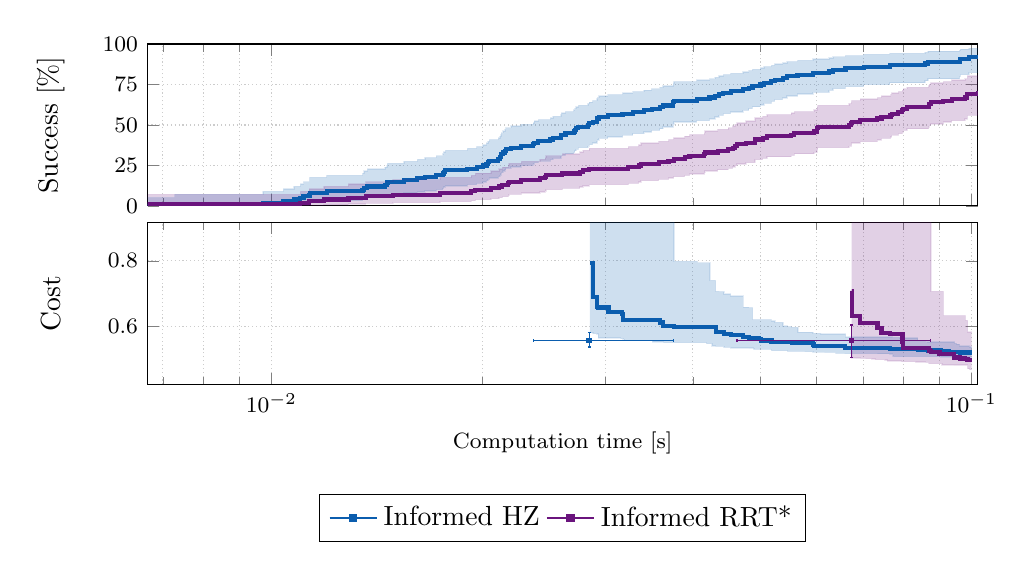
\begin{tikzpicture} [
  xscale=1,
  yscale=1
]
\begin{axis} [
  width=\textwidth,
  height=0.3\textwidth,
  at={(0cm, 0cm)},
  unbounded coords=jump,
  xtick align=inside,
  ytick align=inside,
  axis line style={solid, black},
  name=SuccessAxis,
  xmajorgrids,
  xminorgrids,
  ymajorgrids,
  major grid style={densely dotted, black!20},
  minor grid style={densely dotted, black!20},
  xmin=0.00665588,
  xmax=0.102103,
  ymin=0,
  ymax=100,
  xmode=log,
  xlabel={{\empty}},
  xlabel style={font=\footnotesize},
  xticklabel={{\empty}},
  xticklabel style={font=\footnotesize},
  ylabel={Success [\%]},
  ylabel style={font=\footnotesize, text depth=0.0em, text height=0.5em},
  ylabel absolute,
  ytick={0,25,50,75,100},
  yticklabel style={font=\footnotesize}
]
\addplot [
  line width=0.5,
  color=pdtblue,
  mark="none",
  const plot,
  name path={defaultInformedHZSuccessUpperConfidence},
  fill opacity=0.2,
  draw opacity=0.1
] table [
  row sep=\\,
  col sep=&
]{
1e-09 & 5.1604\\
0.00727877 & 7.19577\\
0.00973225 & 8.94307\\
0.0104066 & 10.5481\\
0.0107682 & 12.0633\\
0.010999 & 13.5145\\
0.0111162 & 14.9169\\
0.0113376 & 16.2803\\
0.0113403 & 17.6114\\
0.0119951 & 18.9152\\
0.013495 & 20.1954\\
0.0135649 & 21.4547\\
0.013711 & 22.6955\\
0.0145303 & 23.9196\\
0.0146348 & 25.1285\\
0.0146493 & 26.3235\\
0.0154656 & 27.5057\\
0.0161594 & 28.676\\
0.0165704 & 29.8351\\
0.0172065 & 30.9838\\
0.0175742 & 32.1226\\
0.0176248 & 33.2522\\
0.0177204 & 34.3729\\
0.0190552 & 35.4851\\
0.0196488 & 36.5893\\
0.0200467 & 37.6857\\
0.0202887 & 38.7747\\
0.020381 & 39.8566\\
0.0204754 & 40.9315\\
0.0211006 & 41.9997\\
0.0212063 & 43.0614\\
0.0212722 & 44.1167\\
0.0213053 & 45.1659\\
0.0214283 & 46.2091\\
0.0215501 & 47.2464\\
0.0216166 & 48.2779\\
0.022005 & 49.3038\\
0.0227139 & 50.3241\\
0.0236598 & 51.339\\
0.0237366 & 52.3485\\
0.0240574 & 53.3527\\
0.0250324 & 54.3517\\
0.0252641 & 55.3454\\
0.0259226 & 56.3341\\
0.0259509 & 57.3177\\
0.0263047 & 58.2962\\
0.0270289 & 59.2697\\
0.0271227 & 60.2382\\
0.0272447 & 61.2017\\
0.0274476 & 62.1603\\
0.0283301 & 63.1139\\
0.0284432 & 64.0625\\
0.0287661 & 65.0062\\
0.0291703 & 65.9449\\
0.0292128 & 66.8786\\
0.0293656 & 67.8073\\
0.0302357 & 68.7309\\
0.0317436 & 69.6495\\
0.0328258 & 70.5629\\
0.0340542 & 71.4712\\
0.0349318 & 72.3742\\
0.0358798 & 73.272\\
0.0362481 & 74.1644\\
0.0374956 & 75.0513\\
0.0375168 & 75.9327\\
0.0375791 & 76.8085\\
0.0405042 & 77.6785\\
0.0422518 & 78.5426\\
0.0430411 & 79.4008\\
0.0435778 & 80.2528\\
0.0442043 & 81.0985\\
0.045286 & 81.9378\\
0.0471368 & 82.7703\\
0.0480712 & 83.596\\
0.0486525 & 84.4145\\
0.0499548 & 85.2256\\
0.0505113 & 86.0291\\
0.0517676 & 86.8245\\
0.0523413 & 87.6116\\
0.0537283 & 88.3899\\
0.0545338 & 89.1589\\
0.056435 & 89.9183\\
0.0593674 & 90.6673\\
0.062623 & 91.4053\\
0.0634351 & 92.1315\\
0.0660638 & 92.8452\\
0.0701477 & 93.5451\\
0.0764454 & 94.2303\\
0.0858301 & 94.8991\\
0.0867008 & 95.5498\\
0.0961613 & 96.1804\\
0.0964124 & 96.7882\\
0.0992366 & 97.3699\\
0.105796 & 97.3699\\
};

\addplot [
  line width=0.5,
  color=pdtblue,
  mark="none",
  const plot,
  name path={defaultInformedHZSuccessLowerConfidence},
  fill opacity=0.2,
  draw opacity=0.1
] table [
  row sep=\\,
  col sep=&
]{
1e-09 & 0\\
0.00727877 & 0.00501242\\
0.00973225 & 0.103962\\
0.0104066 & 0.340707\\
0.0107682 & 0.680169\\
0.010999 & 1.09403\\
0.0111162 & 1.56425\\
0.0113376 & 2.07899\\
0.0113403 & 2.63012\\
0.0119951 & 3.21176\\
0.013495 & 3.81957\\
0.0135649 & 4.45017\\
0.013711 & 5.10094\\
0.0145303 & 5.76975\\
0.0146348 & 6.45486\\
0.0146493 & 7.15483\\
0.0154656 & 7.86846\\
0.0161594 & 8.59473\\
0.0165704 & 9.33274\\
0.0172065 & 10.0817\\
0.0175742 & 10.8411\\
0.0176248 & 11.6101\\
0.0177204 & 12.3884\\
0.0190552 & 13.1755\\
0.0196488 & 13.9709\\
0.0200467 & 14.7744\\
0.0202887 & 15.5855\\
0.020381 & 16.404\\
0.0204754 & 17.2297\\
0.0211006 & 18.0622\\
0.0212063 & 18.9015\\
0.0212722 & 19.7472\\
0.0213053 & 20.5992\\
0.0214283 & 21.4574\\
0.0215501 & 22.3215\\
0.0216166 & 23.1915\\
0.022005 & 24.0673\\
0.0227139 & 24.9487\\
0.0236598 & 25.8356\\
0.0237366 & 26.728\\
0.0240574 & 27.6258\\
0.0250324 & 28.5288\\
0.0252641 & 29.4371\\
0.0259226 & 30.3505\\
0.0259509 & 31.2691\\
0.0263047 & 32.1927\\
0.0270289 & 33.1214\\
0.0271227 & 34.0551\\
0.0272447 & 34.9938\\
0.0274476 & 35.9375\\
0.0283301 & 36.8861\\
0.0284432 & 37.8397\\
0.0287661 & 38.7983\\
0.0291703 & 39.7618\\
0.0292128 & 40.7303\\
0.0293656 & 41.7038\\
0.0302357 & 42.6823\\
0.0317436 & 43.6659\\
0.0328258 & 44.6546\\
0.0340542 & 45.6483\\
0.0349318 & 46.6473\\
0.0358798 & 47.6515\\
0.0362481 & 48.661\\
0.0374956 & 49.6759\\
0.0375168 & 50.6962\\
0.0375791 & 51.7221\\
0.0405042 & 52.7536\\
0.0422518 & 53.7909\\
0.0430411 & 54.8341\\
0.0435778 & 55.8833\\
0.0442043 & 56.9386\\
0.045286 & 58.0003\\
0.0471368 & 59.0685\\
0.0480712 & 60.1434\\
0.0486525 & 61.2253\\
0.0499548 & 62.3143\\
0.0505113 & 63.4107\\
0.0517676 & 64.5149\\
0.0523413 & 65.6271\\
0.0537283 & 66.7478\\
0.0545338 & 67.8774\\
0.056435 & 69.0162\\
0.0593674 & 70.1649\\
0.062623 & 71.324\\
0.0634351 & 72.4943\\
0.0660638 & 73.6765\\
0.0701477 & 74.8715\\
0.0764454 & 76.0804\\
0.0858301 & 77.3045\\
0.0867008 & 78.5453\\
0.0961613 & 79.8046\\
0.0964124 & 81.0848\\
0.0992366 & 82.3886\\
0.105796 & 82.3886\\
};

\addplot [
  line width=1,
  color=pdtblue,
  mark=square*,
  mark size=2,
  const plot,
  fill opacity=0.2,
  draw opacity=0
] fill between [
  of =defaultInformedHZSuccessUpperConfidence and defaultInformedHZSuccessLowerConfidence
];
\addplot [
  line width=1.5,
  color=pdtblue,
  mark="none",
  const plot,
  name path={defaultInformedHZSuccess}
] table [
  row sep=\\,
  col sep=&
]{
1e-09 & 0\\
0.00727877 & 1\\
0.00973225 & 2\\
0.0104066 & 3\\
0.0107682 & 4\\
0.010999 & 5\\
0.0111162 & 6\\
0.0113376 & 7\\
0.0113403 & 8\\
0.0119951 & 9\\
0.013495 & 10\\
0.0135649 & 11\\
0.013711 & 12\\
0.0145303 & 13\\
0.0146348 & 14\\
0.0146493 & 15\\
0.0154656 & 16\\
0.0161594 & 17\\
0.0165704 & 18\\
0.0172065 & 19\\
0.0175742 & 20\\
0.0176248 & 21\\
0.0177204 & 22\\
0.0190552 & 23\\
0.0196488 & 24\\
0.0200467 & 25\\
0.0202887 & 26\\
0.020381 & 27\\
0.0204754 & 28\\
0.0211006 & 29\\
0.0212063 & 30\\
0.0212722 & 31\\
0.0213053 & 32\\
0.0214283 & 33\\
0.0215501 & 34\\
0.0216166 & 35\\
0.022005 & 36\\
0.0227139 & 37\\
0.0236598 & 38\\
0.0237366 & 39\\
0.0240574 & 40\\
0.0250324 & 41\\
0.0252641 & 42\\
0.0259226 & 43\\
0.0259509 & 44\\
0.0263047 & 45\\
0.0270289 & 46\\
0.0271227 & 47\\
0.0272447 & 48\\
0.0274476 & 49\\
0.0283301 & 50\\
0.0284432 & 51\\
0.0287661 & 52\\
0.0291703 & 53\\
0.0292128 & 54\\
0.0293656 & 55\\
0.0302357 & 56\\
0.0317436 & 57\\
0.0328258 & 58\\
0.0340542 & 59\\
0.0349318 & 60\\
0.0358798 & 61\\
0.0362481 & 62\\
0.0374956 & 63\\
0.0375168 & 64\\
0.0375791 & 65\\
0.0405042 & 66\\
0.0422518 & 67\\
0.0430411 & 68\\
0.0435778 & 69\\
0.0442043 & 70\\
0.045286 & 71\\
0.0471368 & 72\\
0.0480712 & 73\\
0.0486525 & 74\\
0.0499548 & 75\\
0.0505113 & 76\\
0.0517676 & 77\\
0.0523413 & 78\\
0.0537283 & 79\\
0.0545338 & 80\\
0.056435 & 81\\
0.0593674 & 82\\
0.062623 & 83\\
0.0634351 & 84\\
0.0660638 & 85\\
0.0701477 & 86\\
0.0764454 & 87\\
0.0858301 & 88\\
0.0867008 & 89\\
0.0961613 & 90\\
0.0964124 & 91\\
0.0992366 & 92\\
0.105796 & 92\\
};

\addplot [
  line width=0.5,
  color=pdtpurple,
  mark="none",
  const plot,
  name path={defaultInformedRRTstarSuccessUpperConfidence},
  fill opacity=0.2,
  draw opacity=0.1
] table [
  row sep=\\,
  col sep=&
]{
1e-09 & 5.1604\\
0.00665588 & 7.19577\\
0.0109981 & 8.94307\\
0.0113252 & 10.5481\\
0.0118879 & 12.0633\\
0.012885 & 13.5145\\
0.0136406 & 14.9169\\
0.0149167 & 16.2803\\
0.0174142 & 17.6114\\
0.0192996 & 18.9152\\
0.0195611 & 20.1954\\
0.0205997 & 21.4547\\
0.0211507 & 22.6955\\
0.0213788 & 23.9196\\
0.0217959 & 25.1285\\
0.0218553 & 26.3235\\
0.0227563 & 27.5057\\
0.0241851 & 28.676\\
0.0246132 & 29.8351\\
0.0246751 & 30.9838\\
0.026039 & 32.1226\\
0.0275755 & 33.2522\\
0.027874 & 34.3729\\
0.0284468 & 35.4851\\
0.0323495 & 36.5893\\
0.0334627 & 37.6857\\
0.0337192 & 38.7747\\
0.0357377 & 39.8566\\
0.0369242 & 40.9315\\
0.0375449 & 41.9997\\
0.0389398 & 43.0614\\
0.0395695 & 44.1167\\
0.0415413 & 45.1659\\
0.0416202 & 46.2091\\
0.0433862 & 47.2464\\
0.0449325 & 48.2779\\
0.0455861 & 49.3038\\
0.0459696 & 50.3241\\
0.0462543 & 51.339\\
0.0476233 & 52.3485\\
0.0490496 & 53.3527\\
0.0490832 & 54.3517\\
0.0503102 & 55.3454\\
0.051061 & 56.3341\\
0.0552754 & 57.3177\\
0.0558574 & 58.2962\\
0.0596094 & 59.2697\\
0.060168 & 60.2382\\
0.0602102 & 61.2017\\
0.0603232 & 62.1603\\
0.0668468 & 63.1139\\
0.0673452 & 64.0625\\
0.0674193 & 65.0062\\
0.0693535 & 65.9449\\
0.0733934 & 66.8786\\
0.0743694 & 67.8073\\
0.0766362 & 68.7309\\
0.0769146 & 69.6495\\
0.0786418 & 70.5629\\
0.0796633 & 71.4712\\
0.0798913 & 72.3742\\
0.0809224 & 73.272\\
0.0868428 & 74.1644\\
0.0870175 & 75.0513\\
0.087436 & 75.9327\\
0.09117 & 76.8085\\
0.093708 & 77.6785\\
0.0979317 & 78.5426\\
0.0986167 & 79.4008\\
0.0986649 & 80.2528\\
0.102103 & 81.0985\\
0.105796 & 81.0985\\
};

\addplot [
  line width=0.5,
  color=pdtpurple,
  mark="none",
  const plot,
  name path={defaultInformedRRTstarSuccessLowerConfidence},
  fill opacity=0.2,
  draw opacity=0.1
] table [
  row sep=\\,
  col sep=&
]{
1e-09 & 0\\
0.00665588 & 0.00501242\\
0.0109981 & 0.103962\\
0.0113252 & 0.340707\\
0.0118879 & 0.680169\\
0.012885 & 1.09403\\
0.0136406 & 1.56425\\
0.0149167 & 2.07899\\
0.0174142 & 2.63012\\
0.0192996 & 3.21176\\
0.0195611 & 3.81957\\
0.0205997 & 4.45017\\
0.0211507 & 5.10094\\
0.0213788 & 5.76975\\
0.0217959 & 6.45486\\
0.0218553 & 7.15483\\
0.0227563 & 7.86846\\
0.0241851 & 8.59473\\
0.0246132 & 9.33274\\
0.0246751 & 10.0817\\
0.026039 & 10.8411\\
0.0275755 & 11.6101\\
0.027874 & 12.3884\\
0.0284468 & 13.1755\\
0.0323495 & 13.9709\\
0.0334627 & 14.7744\\
0.0337192 & 15.5855\\
0.0357377 & 16.404\\
0.0369242 & 17.2297\\
0.0375449 & 18.0622\\
0.0389398 & 18.9015\\
0.0395695 & 19.7472\\
0.0415413 & 20.5992\\
0.0416202 & 21.4574\\
0.0433862 & 22.3215\\
0.0449325 & 23.1915\\
0.0455861 & 24.0673\\
0.0459696 & 24.9487\\
0.0462543 & 25.8356\\
0.0476233 & 26.728\\
0.0490496 & 27.6258\\
0.0490832 & 28.5288\\
0.0503102 & 29.4371\\
0.051061 & 30.3505\\
0.0552754 & 31.2691\\
0.0558574 & 32.1927\\
0.0596094 & 33.1214\\
0.060168 & 34.0551\\
0.0602102 & 34.9938\\
0.0603232 & 35.9375\\
0.0668468 & 36.8861\\
0.0673452 & 37.8397\\
0.0674193 & 38.7983\\
0.0693535 & 39.7618\\
0.0733934 & 40.7303\\
0.0743694 & 41.7038\\
0.0766362 & 42.6823\\
0.0769146 & 43.6659\\
0.0786418 & 44.6546\\
0.0796633 & 45.6483\\
0.0798913 & 46.6473\\
0.0809224 & 47.6515\\
0.0868428 & 48.661\\
0.0870175 & 49.6759\\
0.087436 & 50.6962\\
0.09117 & 51.7221\\
0.093708 & 52.7536\\
0.0979317 & 53.7909\\
0.0986167 & 54.8341\\
0.0986649 & 55.8833\\
0.102103 & 56.9386\\
0.105796 & 56.9386\\
};

\addplot [
  line width=1,
  color=pdtpurple,
  mark=square*,
  mark size=2,
  const plot,
  fill opacity=0.2,
  draw opacity=0
] fill between [
  of =defaultInformedRRTstarSuccessUpperConfidence and defaultInformedRRTstarSuccessLowerConfidence
];
\addplot [
  line width=1.5,
  color=pdtpurple,
  mark="none",
  const plot,
  name path={defaultInformedRRTstarSuccess}
] table [
  row sep=\\,
  col sep=&
]{
1e-09 & 0\\
0.00665588 & 1\\
0.0109981 & 2\\
0.0113252 & 3\\
0.0118879 & 4\\
0.012885 & 5\\
0.0136406 & 6\\
0.0149167 & 7\\
0.0174142 & 8\\
0.0192996 & 9\\
0.0195611 & 10\\
0.0205997 & 11\\
0.0211507 & 12\\
0.0213788 & 13\\
0.0217959 & 14\\
0.0218553 & 15\\
0.0227563 & 16\\
0.0241851 & 17\\
0.0246132 & 18\\
0.0246751 & 19\\
0.026039 & 20\\
0.0275755 & 21\\
0.027874 & 22\\
0.0284468 & 23\\
0.0323495 & 24\\
0.0334627 & 25\\
0.0337192 & 26\\
0.0357377 & 27\\
0.0369242 & 28\\
0.0375449 & 29\\
0.0389398 & 30\\
0.0395695 & 31\\
0.0415413 & 32\\
0.0416202 & 33\\
0.0433862 & 34\\
0.0449325 & 35\\
0.0455861 & 36\\
0.0459696 & 37\\
0.0462543 & 38\\
0.0476233 & 39\\
0.0490496 & 40\\
0.0490832 & 41\\
0.0503102 & 42\\
0.051061 & 43\\
0.0552754 & 44\\
0.0558574 & 45\\
0.0596094 & 46\\
0.060168 & 47\\
0.0602102 & 48\\
0.0603232 & 49\\
0.0668468 & 50\\
0.0673452 & 51\\
0.0674193 & 52\\
0.0693535 & 53\\
0.0733934 & 54\\
0.0743694 & 55\\
0.0766362 & 56\\
0.0769146 & 57\\
0.0786418 & 58\\
0.0796633 & 59\\
0.0798913 & 60\\
0.0809224 & 61\\
0.0868428 & 62\\
0.0870175 & 63\\
0.087436 & 64\\
0.09117 & 65\\
0.093708 & 66\\
0.0979317 & 67\\
0.0986167 & 68\\
0.0986649 & 69\\
0.102103 & 70\\
0.105796 & 70\\
};

\end{axis}

\begin{axis} [
  width=\textwidth,
  height=0.3\textwidth,
  at={($(SuccessAxis.south) - (0.0em, 0.6em)$)},
  unbounded coords=jump,
  xtick align=inside,
  ytick align=inside,
  axis line style={solid, black},
  name=AllPlannersMedianCostAxis,
  anchor=north,
  xmajorgrids,
  xminorgrids,
  ymajorgrids,
  major grid style={densely dotted, black!20},
  minor grid style={densely dotted, black!20},
  xmin=0.00665588,
  xmax=0.102103,
  ymax=0.917277,
  xmode=log,
  xlabel={Computation time [s]},
  xlabel style={font=\footnotesize},
  xticklabel style={font=\footnotesize},
  ylabel={Cost},
  ylabel style={font=\footnotesize, text depth=0.0em, text height=0.5em},
  ylabel absolute,
  yticklabel style={font=\footnotesize}
]
\addplot [
  line width=0.5,
  color=pdtblue,
  mark="none",
  const plot,
  name path={defaultInformedHZMedianCostEvolutionUpperConfidence},
  fill opacity=0.2,
  draw opacity=0.1
] table [
  row sep=\\,
  col sep=&
]{
0.0285 & 2.75183\\
0.0375 & 2.75183\\
0.0376 & 0.798258\\
0.0405 & 0.798258\\
0.0406 & 0.794084\\
0.0422 & 0.794084\\
0.0423 & 0.739939\\
0.043 & 0.739939\\
0.0431 & 0.706615\\
0.0435 & 0.706615\\
0.0436 & 0.705923\\
0.0442 & 0.705923\\
0.0443 & 0.698113\\
0.0452 & 0.698113\\
0.0453 & 0.691929\\
0.0471 & 0.691929\\
0.0472 & 0.658085\\
0.048 & 0.658085\\
0.0481 & 0.657134\\
0.0486 & 0.657134\\
0.0487 & 0.620054\\
0.0499 & 0.620054\\
0.05 & 0.619746\\
0.0517 & 0.619746\\
0.0518 & 0.61631\\
0.0523 & 0.61631\\
0.0524 & 0.611343\\
0.0537 & 0.611343\\
0.0538 & 0.600178\\
0.0545 & 0.600178\\
0.0546 & 0.598686\\
0.0552 & 0.598686\\
0.0553 & 0.596429\\
0.0564 & 0.596429\\
0.0565 & 0.58157\\
0.0593 & 0.58157\\
0.0594 & 0.577879\\
0.0609 & 0.577879\\
0.061 & 0.576081\\
0.066 & 0.576081\\
0.0661 & 0.56672\\
0.0701 & 0.56672\\
0.0702 & 0.566717\\
0.0756 & 0.566717\\
0.0757 & 0.56671\\
0.0758 & 0.566682\\
0.0759 & 0.566674\\
0.0764 & 0.566674\\
0.0765 & 0.566673\\
0.077 & 0.566673\\
0.0771 & 0.565966\\
0.079 & 0.565966\\
0.0791 & 0.563993\\
0.0837 & 0.563993\\
0.0838 & 0.556215\\
0.0858 & 0.556215\\
0.0859 & 0.552257\\
0.0864 & 0.552257\\
0.0865 & 0.55181\\
0.0926 & 0.55181\\
0.0927 & 0.551736\\
0.0945 & 0.551736\\
0.0946 & 0.547667\\
0.0951 & 0.547667\\
0.0952 & 0.544896\\
0.0961 & 0.544896\\
0.0962 & 0.539373\\
0.0992 & 0.539373\\
0.0993 & 0.536932\\
0.0994 & 0.536446\\
0.0999 & 0.536446\\
0.1 & 0.536446\\
};

\addplot [
  line width=0.5,
  color=pdtblue,
  mark="none",
  const plot,
  name path={defaultInformedHZMedianCostEvolutionLowerConfidence},
  fill opacity=0.2,
  draw opacity=0.1
] table [
  row sep=\\,
  col sep=&
]{
0.0285 & 0.57989\\
0.0287 & 0.57989\\
0.0288 & 0.577043\\
0.0291 & 0.577043\\
0.0292 & 0.576249\\
0.0293 & 0.563993\\
0.0314 & 0.563993\\
0.0315 & 0.563041\\
0.0316 & 0.561789\\
0.0317 & 0.561789\\
0.0318 & 0.560175\\
0.0319 & 0.556215\\
0.0349 & 0.556215\\
0.035 & 0.55181\\
0.0362 & 0.55181\\
0.0363 & 0.54964\\
0.0417 & 0.54964\\
0.0418 & 0.546921\\
0.0425 & 0.546921\\
0.0426 & 0.539897\\
0.0429 & 0.539897\\
0.043 & 0.53937\\
0.0431 & 0.538233\\
0.0432 & 0.537986\\
0.0442 & 0.537986\\
0.0443 & 0.534868\\
0.0452 & 0.534868\\
0.0453 & 0.533555\\
0.048 & 0.533555\\
0.0481 & 0.533024\\
0.0487 & 0.533024\\
0.0488 & 0.530883\\
0.0489 & 0.529306\\
0.0499 & 0.529306\\
0.05 & 0.529119\\
0.0517 & 0.529119\\
0.0518 & 0.52546\\
0.0545 & 0.52546\\
0.0546 & 0.522901\\
0.0577 & 0.522901\\
0.0578 & 0.522418\\
0.0593 & 0.522418\\
0.0594 & 0.520386\\
0.0616 & 0.520386\\
0.0617 & 0.519575\\
0.0639 & 0.519575\\
0.064 & 0.517087\\
0.0658 & 0.517087\\
0.0659 & 0.516025\\
0.0701 & 0.516025\\
0.0702 & 0.515683\\
0.0733 & 0.515683\\
0.0734 & 0.515575\\
0.0764 & 0.515575\\
0.0765 & 0.51443\\
0.0771 & 0.51443\\
0.0772 & 0.510899\\
0.0773 & 0.507983\\
0.0774 & 0.50716\\
0.0878 & 0.50716\\
0.0879 & 0.507109\\
0.0904 & 0.507109\\
0.0905 & 0.505948\\
0.0927 & 0.505948\\
0.0928 & 0.505837\\
0.0961 & 0.505837\\
0.0962 & 0.505274\\
0.0985 & 0.505274\\
0.0986 & 0.505138\\
0.0994 & 0.505138\\
0.0995 & 0.504591\\
0.0999 & 0.504591\\
0.1 & 0.504591\\
};

\addplot [
  line width=1,
  color=pdtblue,
  mark=square*,
  mark size=2,
  const plot,
  fill opacity=0.2,
  draw opacity=0
] fill between [
  of =defaultInformedHZMedianCostEvolutionUpperConfidence and defaultInformedHZMedianCostEvolutionLowerConfidence
];
\addplot [
  line width=1.5,
  color=pdtblue,
  mark="none",
  const plot,
  name path={defaultInformedHZMedianCostEvolution}
] table [
  row sep=\\,
  col sep=&
]{
0.0001 & inf\\
0.0284 & inf\\
0.0285 & 0.794084\\
0.0287 & 0.794084\\
0.0288 & 0.689022\\
0.0291 & 0.689022\\
0.0292 & 0.658085\\
0.0293 & 0.657134\\
0.0302 & 0.657134\\
0.0303 & 0.642834\\
0.0316 & 0.642834\\
0.0317 & 0.636556\\
0.0318 & 0.620054\\
0.0349 & 0.620054\\
0.035 & 0.619746\\
0.0358 & 0.619746\\
0.0359 & 0.611343\\
0.0362 & 0.611343\\
0.0363 & 0.600178\\
0.0375 & 0.600178\\
0.0376 & 0.598686\\
0.0428 & 0.598686\\
0.0429 & 0.596429\\
0.043 & 0.596429\\
0.0431 & 0.58157\\
0.0442 & 0.58157\\
0.0443 & 0.576081\\
0.0452 & 0.576081\\
0.0453 & 0.572326\\
0.0471 & 0.572326\\
0.0472 & 0.566717\\
0.0473 & 0.565966\\
0.048 & 0.565966\\
0.0481 & 0.563993\\
0.0496 & 0.563993\\
0.0497 & 0.561193\\
0.0499 & 0.561193\\
0.05 & 0.556215\\
0.0517 & 0.556215\\
0.0518 & 0.55181\\
0.0545 & 0.55181\\
0.0546 & 0.551296\\
0.0553 & 0.551296\\
0.0554 & 0.54964\\
0.0577 & 0.54964\\
0.0578 & 0.547667\\
0.0593 & 0.547667\\
0.0594 & 0.54416\\
0.0595 & 0.53937\\
0.0638 & 0.53937\\
0.0639 & 0.538233\\
0.0658 & 0.538233\\
0.0659 & 0.534419\\
0.066 & 0.534419\\
0.0661 & 0.533807\\
0.0701 & 0.533807\\
0.0702 & 0.533555\\
0.0746 & 0.533555\\
0.0747 & 0.533438\\
0.0748 & 0.532999\\
0.0764 & 0.532999\\
0.0765 & 0.529306\\
0.0771 & 0.529306\\
0.0772 & 0.529119\\
0.0837 & 0.529119\\
0.0838 & 0.527665\\
0.0865 & 0.527665\\
0.0866 & 0.52546\\
0.0904 & 0.52546\\
0.0905 & 0.522901\\
0.0927 & 0.522901\\
0.0928 & 0.520386\\
0.0946 & 0.520386\\
0.0947 & 0.519937\\
0.0961 & 0.519937\\
0.0962 & 0.519575\\
0.0994 & 0.519575\\
0.0995 & 0.517447\\
0.0999 & 0.517447\\
0.1 & 0.517447\\
};

\addplot [
  line width=0.5,
  color=pdtpurple,
  mark="none",
  const plot,
  name path={defaultInformedRRTstarMedianCostEvolutionUpperConfidence},
  fill opacity=0.2,
  draw opacity=0.1
] table [
  row sep=\\,
  col sep=&
]{
0.0674 & 2.75183\\
0.0874 & 2.75183\\
0.0875 & 0.70681\\
0.0911 & 0.70681\\
0.0912 & 0.632282\\
0.0979 & 0.632282\\
0.098 & 0.618009\\
0.0986 & 0.618009\\
0.0987 & 0.582012\\
0.0999 & 0.582012\\
0.1 & 0.582012\\
};

\addplot [
  line width=0.5,
  color=pdtpurple,
  mark="none",
  const plot,
  name path={defaultInformedRRTstarMedianCostEvolutionLowerConfidence},
  fill opacity=0.2,
  draw opacity=0.1
] table [
  row sep=\\,
  col sep=&
]{
0.0674 & 0.521862\\
0.0675 & 0.503083\\
0.0682 & 0.503083\\
0.0683 & 0.50254\\
0.0693 & 0.50254\\
0.0694 & 0.501393\\
0.0705 & 0.501393\\
0.0706 & 0.500978\\
0.0707 & 0.500392\\
0.0719 & 0.500392\\
0.072 & 0.500104\\
0.0723 & 0.500104\\
0.0724 & 0.499767\\
0.0727 & 0.499767\\
0.0728 & 0.497793\\
0.073 & 0.497793\\
0.0731 & 0.49779\\
0.0751 & 0.49779\\
0.0752 & 0.496947\\
0.0753 & 0.496347\\
0.0756 & 0.496347\\
0.0757 & 0.495435\\
0.0758 & 0.493925\\
0.0792 & 0.493925\\
0.0793 & 0.492915\\
0.0794 & 0.491447\\
0.081 & 0.491447\\
0.0811 & 0.491396\\
0.0831 & 0.491396\\
0.0832 & 0.490227\\
0.0859 & 0.490227\\
0.086 & 0.489312\\
0.0868 & 0.489312\\
0.0869 & 0.48537\\
0.0906 & 0.48537\\
0.0907 & 0.481489\\
0.0943 & 0.481489\\
0.0944 & 0.480687\\
0.0986 & 0.480687\\
0.0987 & 0.469659\\
0.0993 & 0.469659\\
0.0994 & 0.46715\\
0.0997 & 0.46715\\
0.0998 & 0.466826\\
0.0999 & 0.466826\\
0.1 & 0.466826\\
};

\addplot [
  line width=1,
  color=pdtpurple,
  mark=square*,
  mark size=2,
  const plot,
  fill opacity=0.2,
  draw opacity=0
] fill between [
  of =defaultInformedRRTstarMedianCostEvolutionUpperConfidence and defaultInformedRRTstarMedianCostEvolutionLowerConfidence
];
\addplot [
  line width=1.5,
  color=pdtpurple,
  mark="none",
  const plot,
  name path={defaultInformedRRTstarMedianCostEvolution}
] table [
  row sep=\\,
  col sep=&
]{
0.0001 & inf\\
0.0673 & inf\\
0.0674 & 0.70681\\
0.0675 & 0.632282\\
0.0693 & 0.632282\\
0.0694 & 0.609362\\
0.0733 & 0.609362\\
0.0734 & 0.595264\\
0.0743 & 0.595264\\
0.0744 & 0.579349\\
0.0763 & 0.579349\\
0.0764 & 0.576959\\
0.0796 & 0.576959\\
0.0797 & 0.551503\\
0.0798 & 0.551503\\
0.0799 & 0.532992\\
0.0868 & 0.532992\\
0.0869 & 0.525694\\
0.087 & 0.525694\\
0.0871 & 0.524031\\
0.0874 & 0.524031\\
0.0875 & 0.520627\\
0.0899 & 0.520627\\
0.09 & 0.515762\\
0.0905 & 0.515762\\
0.0906 & 0.515218\\
0.0937 & 0.515218\\
0.0938 & 0.513841\\
0.0942 & 0.513841\\
0.0943 & 0.504322\\
0.0962 & 0.504322\\
0.0963 & 0.500973\\
0.0979 & 0.500973\\
0.098 & 0.500019\\
0.0986 & 0.500019\\
0.0987 & 0.49779\\
0.0992 & 0.49779\\
0.0993 & 0.496798\\
0.0999 & 0.496798\\
0.1 & 0.496798\\
};

\addplot [
  line width=1,
  color=pdtblue,
  mark=square*,
  mark size=0.5,
  only marks,
  const plot,
  name path={defaultInformedHZMedianInitialSolution}
] table [
  row sep=\\,
  col sep=&
]{
0.0284432 & 0.556215\\
};

\addplot [
  line width=0.5,
  color=pdtblue,
  mark=|,
  mark size=0.5,
  const plot,
  name path={defaultInformedHZMedianInitialSolutionDurationConfidenceInterval}
] table [
  row sep=\\,
  col sep=&
]{
0.0236598 & 0.556215\\
0.0375168 & 0.556215\\
};

\addplot [
  line width=0.5,
  color=pdtblue,
  mark=-,
  mark size=0.5,
  const plot,
  name path={defaultInformedHZMedianInitialSolutionDurationConfidenceInterval}
] table [
  row sep=\\,
  col sep=&
]{
0.0284432 & 0.536446\\
0.0284432 & 0.58157\\
};

\addplot [
  line width=1,
  color=pdtpurple,
  mark=square*,
  mark size=0.5,
  only marks,
  const plot,
  name path={defaultInformedRRTstarMedianInitialSolution}
] table [
  row sep=\\,
  col sep=&
]{
0.0673452 & 0.55676\\
};

\addplot [
  line width=0.5,
  color=pdtpurple,
  mark=|,
  mark size=0.5,
  const plot,
  name path={defaultInformedRRTstarMedianInitialSolutionDurationConfidenceInterval}
] table [
  row sep=\\,
  col sep=&
]{
0.0462543 & 0.55676\\
0.087436 & 0.55676\\
};

\addplot [
  line width=0.5,
  color=pdtpurple,
  mark=-,
  mark size=0.5,
  const plot,
  name path={defaultInformedRRTstarMedianInitialSolutionDurationConfidenceInterval}
] table [
  row sep=\\,
  col sep=&
]{
0.0673452 & 0.50478\\
0.0673452 & 0.603475\\
};

\end{axis}

\begin{axis} [
  width=\textwidth,
  height=0.5\textwidth,
  at={($(AllPlannersMedianCostAxis.south) - (0.0em, 0.6em)$)},
  unbounded coords=jump,
  xtick align=inside,
  ytick align=inside,
  axis line style={solid, black},
  anchor=north,
  hide axis,
  xmajorgrids,
  ymajorgrids,
  major grid style={densely dotted, black!20},
  xmin=0,
  xmax=10,
  ymin=0,
  ymax=10,
  xlabel style={font=\footnotesize},
  xticklabel style={font=\footnotesize},
  ylabel style={font=\footnotesize},
  yticklabel style={font=\footnotesize},
  legend style={anchor=south, legend cell align=left, legend columns=-1, at={(axis cs:5, 6)}}
]
\addlegendimage{pdtblue, line width = 1.0pt, mark size=1.0pt, mark=square*}
\addlegendentry{Informed HZ}
\addlegendimage{pdtpurple, line width = 1.0pt, mark size=1.0pt, mark=square*}
\addlegendentry{Informed RRT*}
\end{axis}

\end{tikzpicture}%
\captionof{figure}{\footnotesize \textbf{Top:} Percentage of runs that found a solution at any given time with a Clopper-Pearson (nonparametric) 99\% confidence interval. \textbf{Bottom:} Median cost evolution and median of initial solution with nonparametric 99\% confidence intervals.}
\end{center}
\pagebreak
\subsection{Initial Solutions}\label{sec:overview-initial-solutions}
\begin{center}
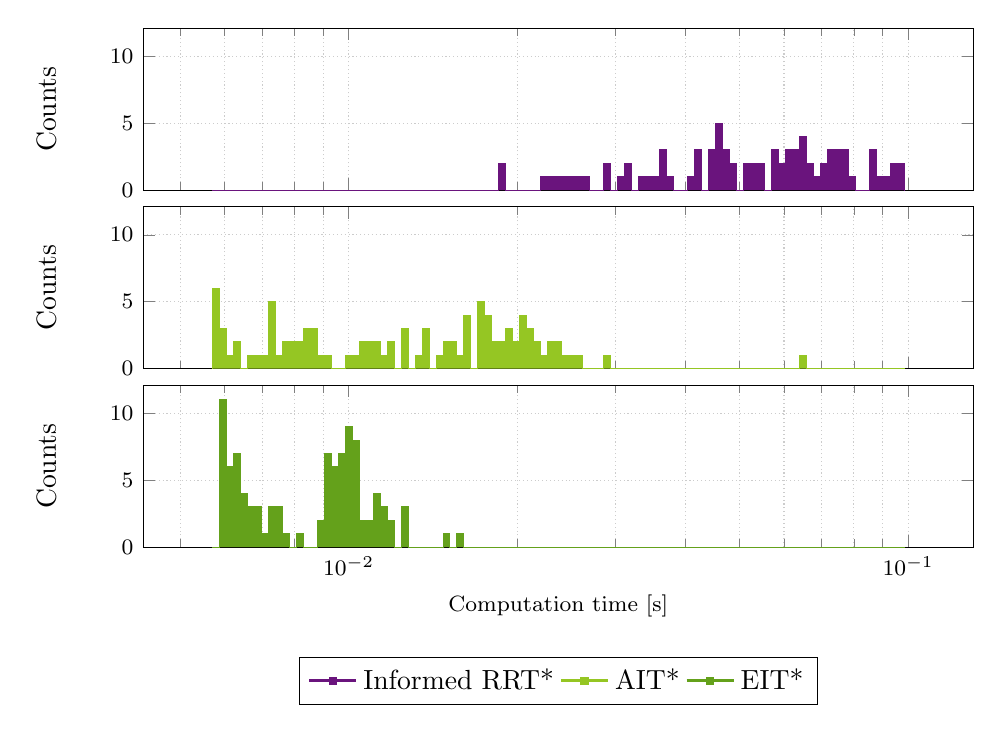
\begin{tikzpicture} [
  xscale=1,
  yscale=1
]
\begin{axis} [
  width=\textwidth,
  height=0.3\textwidth,
  at={(0cm, 0cm)},
  unbounded coords=jump,
  xtick align=inside,
  ytick align=inside,
  axis line style={solid, black},
  name=defaultInformedRRTstarISDPA,
  xmajorgrids,
  xminorgrids,
  ymajorgrids,
  major grid style={densely dotted, black!20},
  minor grid style={densely dotted, black!20},
  ymin=0,
  ymax=11,
  enlarge y limits=upper,
  xmode=log,
  xlabel={{\empty}},
  xlabel style={font=\footnotesize},
  xticklabel={{\empty}},
  xticklabel style={font=\footnotesize},
  ylabel={Counts},
  ylabel style={font=\footnotesize, text depth=0.0em, text height=0.5em},
  ylabel absolute,
  yticklabel style={font=\footnotesize}
]
\addplot [
  line width=0,
  color=pdtpurple,
  mark="none",
  const plot,
  name path={defaultInformedRRTstarInitialSolutionDurationHistogram},
  fill=pdtpurple
] table [
  row sep=\\,
  col sep=&
]{
0.00570601 & 0\\
0.00570601 & 0\\
0.00587252 & 0\\
0.0060439 & 0\\
0.00622027 & 0\\
0.00640179 & 0\\
0.00658861 & 0\\
0.00678089 & 0\\
0.00697877 & 0\\
0.00718243 & 0\\
0.00739203 & 0\\
0.00760774 & 0\\
0.00782975 & 0\\
0.00805825 & 0\\
0.0082934 & 0\\
0.00853543 & 0\\
0.00878451 & 0\\
0.00904086 & 0\\
0.0093047 & 0\\
0.00957623 & 0\\
0.00985569 & 0\\
0.0101433 & 0\\
0.0104393 & 0\\
0.0107439 & 0\\
0.0110575 & 0\\
0.0113802 & 0\\
0.0117123 & 0\\
0.0120541 & 0\\
0.0124058 & 0\\
0.0127679 & 0\\
0.0131405 & 0\\
0.0135239 & 0\\
0.0139186 & 0\\
0.0143248 & 0\\
0.0147428 & 0\\
0.015173 & 0\\
0.0156158 & 0\\
0.0160715 & 0\\
0.0165405 & 0\\
0.0170232 & 0\\
0.01752 & 0\\
0.0180313 & 0\\
0.0185575 & 2\\
0.019099 & 0\\
0.0196564 & 0\\
0.02023 & 0\\
0.0208203 & 0\\
0.0214279 & 0\\
0.0220532 & 1\\
0.0226968 & 1\\
0.0233592 & 1\\
0.0240408 & 1\\
0.0247424 & 1\\
0.0254644 & 1\\
0.0262076 & 1\\
0.0269724 & 0\\
0.0277595 & 0\\
0.0285696 & 2\\
0.0294033 & 0\\
0.0302613 & 1\\
0.0311444 & 2\\
0.0320533 & 0\\
0.0329887 & 1\\
0.0339514 & 1\\
0.0349422 & 1\\
0.0359619 & 3\\
0.0370113 & 1\\
0.0380914 & 0\\
0.039203 & 0\\
0.040347 & 1\\
0.0415245 & 3\\
0.0427362 & 0\\
0.0439834 & 3\\
0.0452669 & 5\\
0.0465879 & 3\\
0.0479475 & 2\\
0.0493467 & 0\\
0.0507867 & 2\\
0.0522688 & 2\\
0.0537941 & 2\\
0.055364 & 0\\
0.0569796 & 3\\
0.0586424 & 2\\
0.0603538 & 3\\
0.062115 & 3\\
0.0639277 & 4\\
0.0657933 & 2\\
0.0677133 & 1\\
0.0696893 & 2\\
0.071723 & 3\\
0.073816 & 3\\
0.0759702 & 3\\
0.0781872 & 1\\
0.0804688 & 0\\
0.0828171 & 0\\
0.0852339 & 3\\
0.0877213 & 1\\
0.0902812 & 1\\
0.0929158 & 2\\
0.0956273 & 2\\
0.0984179 & 0\\
0.0984179 & 0\\
};

\end{axis}

\begin{axis} [
  width=\textwidth,
  height=0.3\textwidth,
  at={($(defaultInformedRRTstarISDPA.south) - (0.0em, 0.6em)$)},
  unbounded coords=jump,
  xtick align=inside,
  ytick align=inside,
  axis line style={solid, black},
  name=defaultAITstarISDPA,
  anchor=north,
  xmajorgrids,
  xminorgrids,
  ymajorgrids,
  major grid style={densely dotted, black!20},
  minor grid style={densely dotted, black!20},
  ymin=0,
  ymax=11,
  enlarge y limits=upper,
  xmode=log,
  xlabel={{\empty}},
  xlabel style={font=\footnotesize},
  xticklabel={{\empty}},
  xticklabel style={font=\footnotesize},
  ylabel={Counts},
  ylabel style={font=\footnotesize, text depth=0.0em, text height=0.5em},
  ylabel absolute,
  yticklabel style={font=\footnotesize}
]
\addplot [
  line width=0,
  color=pdtlightgreen,
  mark="none",
  const plot,
  name path={defaultAITstarInitialSolutionDurationHistogram},
  fill=pdtlightgreen
] table [
  row sep=\\,
  col sep=&
]{
0.00570601 & 0\\
0.00570601 & 6\\
0.00587252 & 3\\
0.0060439 & 1\\
0.00622027 & 2\\
0.00640179 & 0\\
0.00658861 & 1\\
0.00678089 & 1\\
0.00697877 & 1\\
0.00718243 & 5\\
0.00739203 & 1\\
0.00760774 & 2\\
0.00782975 & 2\\
0.00805825 & 2\\
0.0082934 & 3\\
0.00853543 & 3\\
0.00878451 & 1\\
0.00904086 & 1\\
0.0093047 & 0\\
0.00957623 & 0\\
0.00985569 & 1\\
0.0101433 & 1\\
0.0104393 & 2\\
0.0107439 & 2\\
0.0110575 & 2\\
0.0113802 & 1\\
0.0117123 & 2\\
0.0120541 & 0\\
0.0124058 & 3\\
0.0127679 & 0\\
0.0131405 & 1\\
0.0135239 & 3\\
0.0139186 & 0\\
0.0143248 & 1\\
0.0147428 & 2\\
0.015173 & 2\\
0.0156158 & 1\\
0.0160715 & 4\\
0.0165405 & 0\\
0.0170232 & 5\\
0.01752 & 4\\
0.0180313 & 2\\
0.0185575 & 2\\
0.019099 & 3\\
0.0196564 & 2\\
0.02023 & 4\\
0.0208203 & 3\\
0.0214279 & 2\\
0.0220532 & 1\\
0.0226968 & 2\\
0.0233592 & 2\\
0.0240408 & 1\\
0.0247424 & 1\\
0.0254644 & 1\\
0.0262076 & 0\\
0.0269724 & 0\\
0.0277595 & 0\\
0.0285696 & 1\\
0.0294033 & 0\\
0.0302613 & 0\\
0.0311444 & 0\\
0.0320533 & 0\\
0.0329887 & 0\\
0.0339514 & 0\\
0.0349422 & 0\\
0.0359619 & 0\\
0.0370113 & 0\\
0.0380914 & 0\\
0.039203 & 0\\
0.040347 & 0\\
0.0415245 & 0\\
0.0427362 & 0\\
0.0439834 & 0\\
0.0452669 & 0\\
0.0465879 & 0\\
0.0479475 & 0\\
0.0493467 & 0\\
0.0507867 & 0\\
0.0522688 & 0\\
0.0537941 & 0\\
0.055364 & 0\\
0.0569796 & 0\\
0.0586424 & 0\\
0.0603538 & 0\\
0.062115 & 0\\
0.0639277 & 1\\
0.0657933 & 0\\
0.0677133 & 0\\
0.0696893 & 0\\
0.071723 & 0\\
0.073816 & 0\\
0.0759702 & 0\\
0.0781872 & 0\\
0.0804688 & 0\\
0.0828171 & 0\\
0.0852339 & 0\\
0.0877213 & 0\\
0.0902812 & 0\\
0.0929158 & 0\\
0.0956273 & 0\\
0.0984179 & 0\\
0.0984179 & 0\\
};

\end{axis}

\begin{axis} [
  width=\textwidth,
  height=0.3\textwidth,
  at={($(defaultAITstarISDPA.south) - (0.0em, 0.6em)$)},
  unbounded coords=jump,
  xtick align=inside,
  ytick align=inside,
  axis line style={solid, black},
  name=defaultEITstarISDPA,
  anchor=north,
  xmajorgrids,
  xminorgrids,
  ymajorgrids,
  major grid style={densely dotted, black!20},
  minor grid style={densely dotted, black!20},
  ymin=0,
  ymax=11,
  enlarge y limits=upper,
  xmode=log,
  xlabel={Computation time [s]},
  xlabel style={font=\footnotesize},
  xticklabel style={font=\footnotesize},
  ylabel={Counts},
  ylabel style={font=\footnotesize, text depth=0.0em, text height=0.5em},
  ylabel absolute,
  yticklabel style={font=\footnotesize}
]
\addplot [
  line width=0,
  color=pdtgreen,
  mark="none",
  const plot,
  name path={defaultEITstarInitialSolutionDurationHistogram},
  fill=pdtgreen
] table [
  row sep=\\,
  col sep=&
]{
0.00570601 & 0\\
0.00570601 & 0\\
0.00587252 & 11\\
0.0060439 & 6\\
0.00622027 & 7\\
0.00640179 & 4\\
0.00658861 & 3\\
0.00678089 & 3\\
0.00697877 & 1\\
0.00718243 & 3\\
0.00739203 & 3\\
0.00760774 & 1\\
0.00782975 & 0\\
0.00805825 & 1\\
0.0082934 & 0\\
0.00853543 & 0\\
0.00878451 & 2\\
0.00904086 & 7\\
0.0093047 & 6\\
0.00957623 & 7\\
0.00985569 & 9\\
0.0101433 & 8\\
0.0104393 & 2\\
0.0107439 & 2\\
0.0110575 & 4\\
0.0113802 & 3\\
0.0117123 & 2\\
0.0120541 & 0\\
0.0124058 & 3\\
0.0127679 & 0\\
0.0131405 & 0\\
0.0135239 & 0\\
0.0139186 & 0\\
0.0143248 & 0\\
0.0147428 & 1\\
0.015173 & 0\\
0.0156158 & 1\\
0.0160715 & 0\\
0.0165405 & 0\\
0.0170232 & 0\\
0.01752 & 0\\
0.0180313 & 0\\
0.0185575 & 0\\
0.019099 & 0\\
0.0196564 & 0\\
0.02023 & 0\\
0.0208203 & 0\\
0.0214279 & 0\\
0.0220532 & 0\\
0.0226968 & 0\\
0.0233592 & 0\\
0.0240408 & 0\\
0.0247424 & 0\\
0.0254644 & 0\\
0.0262076 & 0\\
0.0269724 & 0\\
0.0277595 & 0\\
0.0285696 & 0\\
0.0294033 & 0\\
0.0302613 & 0\\
0.0311444 & 0\\
0.0320533 & 0\\
0.0329887 & 0\\
0.0339514 & 0\\
0.0349422 & 0\\
0.0359619 & 0\\
0.0370113 & 0\\
0.0380914 & 0\\
0.039203 & 0\\
0.040347 & 0\\
0.0415245 & 0\\
0.0427362 & 0\\
0.0439834 & 0\\
0.0452669 & 0\\
0.0465879 & 0\\
0.0479475 & 0\\
0.0493467 & 0\\
0.0507867 & 0\\
0.0522688 & 0\\
0.0537941 & 0\\
0.055364 & 0\\
0.0569796 & 0\\
0.0586424 & 0\\
0.0603538 & 0\\
0.062115 & 0\\
0.0639277 & 0\\
0.0657933 & 0\\
0.0677133 & 0\\
0.0696893 & 0\\
0.071723 & 0\\
0.073816 & 0\\
0.0759702 & 0\\
0.0781872 & 0\\
0.0804688 & 0\\
0.0828171 & 0\\
0.0852339 & 0\\
0.0877213 & 0\\
0.0902812 & 0\\
0.0929158 & 0\\
0.0956273 & 0\\
0.0984179 & 0\\
0.0984179 & 0\\
};

\end{axis}

\begin{axis} [
  width=\textwidth,
  height=0.5\textwidth,
  at={($(defaultEITstarISDPA.south) - (0.0em, 0.6em)$)},
  unbounded coords=jump,
  xtick align=inside,
  ytick align=inside,
  axis line style={solid, black},
  anchor=north,
  hide axis,
  xmajorgrids,
  ymajorgrids,
  major grid style={densely dotted, black!20},
  xmin=0,
  xmax=10,
  ymin=0,
  ymax=10,
  xlabel style={font=\footnotesize},
  xticklabel style={font=\footnotesize},
  ylabel style={font=\footnotesize},
  yticklabel style={font=\footnotesize},
  legend style={anchor=south, legend cell align=left, legend columns=-1, at={(axis cs:5, 6)}}
]
\addlegendimage{pdtpurple, line width = 1.0pt, mark size=1.0pt, mark=square*}
\addlegendentry{Informed RRT*}
\addlegendimage{pdtlightgreen, line width = 1.0pt, mark size=1.0pt, mark=square*}
\addlegendentry{AIT*}
\addlegendimage{pdtgreen, line width = 1.0pt, mark size=1.0pt, mark=square*}
\addlegendentry{EIT*}
\end{axis}

\end{tikzpicture}%
\captionof{figure}{\footnotesize Histograms of initial solution times.}
\end{center}
\pagebreak
\section{Informed RRT*}\label{sec:defaultInformedRRTstar}
\subsection{Initial Solutions}\label{sec:defaultInformedRRTstar-initial-solution}
\begin{center}
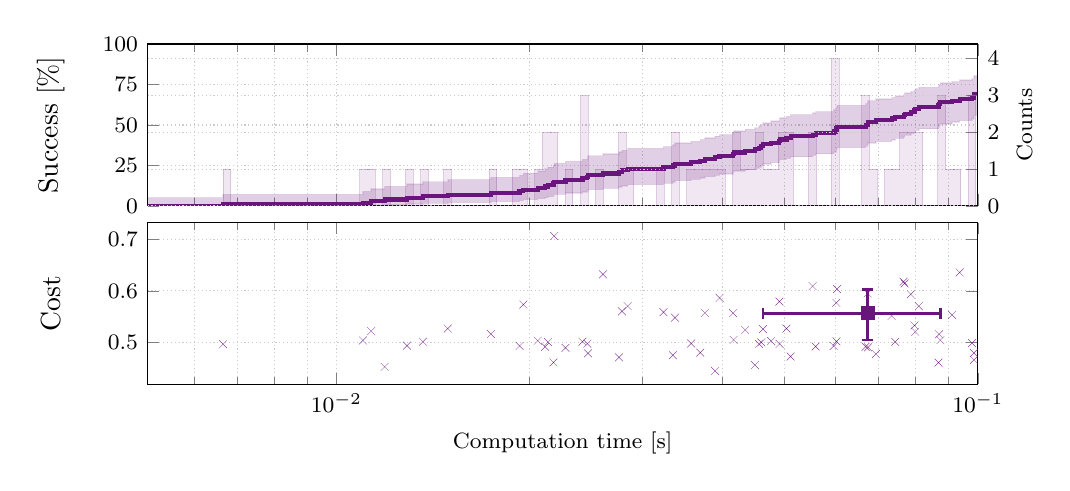
\begin{tikzpicture} [
  xscale=1,
  yscale=1
]
\begin{axis} [
  width=\textwidth,
  height=0.3\textwidth,
  at={(0cm, 0cm)},
  unbounded coords=jump,
  xtick align=inside,
  ytick align=inside,
  axis line style={solid, black},
  name=SuccessAxis,
  xmajorgrids,
  xminorgrids,
  ymajorgrids,
  major grid style={densely dotted, black!20},
  minor grid style={densely dotted, black!20},
  xmin=0.00665588,
  xmax=0.1,
  enlarge x limits=lower,
  ymin=0,
  ymax=100,
  xmode=log,
  xlabel={{\empty}},
  xlabel style={font=\footnotesize},
  xticklabel={{\empty}},
  xticklabel style={font=\footnotesize},
  ylabel={Success [\%]},
  ylabel style={font=\footnotesize, text depth=0.0em, text height=0.5em},
  ylabel absolute,
  ytick={0,25,50,75,100},
 ytick pos={left},
  yticklabel style={font=\footnotesize}
]
\addplot [
  line width=0.5,
  color=pdtpurple,
  mark="none",
  const plot,
  name path={defaultInformedRRTstarSuccessUpperConfidence},
  fill opacity=0.2,
  draw opacity=0.1
] table [
  row sep=\\,
  col sep=&
]{
1e-09 & 5.1604\\
0.00665588 & 7.19577\\
0.0109981 & 8.94307\\
0.0113252 & 10.5481\\
0.0118879 & 12.0633\\
0.012885 & 13.5145\\
0.0136406 & 14.9169\\
0.0149167 & 16.2803\\
0.0174142 & 17.6114\\
0.0192996 & 18.9152\\
0.0195611 & 20.1954\\
0.0205997 & 21.4547\\
0.0211507 & 22.6955\\
0.0213788 & 23.9196\\
0.0217959 & 25.1285\\
0.0218553 & 26.3235\\
0.0227563 & 27.5057\\
0.0241851 & 28.676\\
0.0246132 & 29.8351\\
0.0246751 & 30.9838\\
0.026039 & 32.1226\\
0.0275755 & 33.2522\\
0.027874 & 34.3729\\
0.0284468 & 35.4851\\
0.0323495 & 36.5893\\
0.0334627 & 37.6857\\
0.0337192 & 38.7747\\
0.0357377 & 39.8566\\
0.0369242 & 40.9315\\
0.0375449 & 41.9997\\
0.0389398 & 43.0614\\
0.0395695 & 44.1167\\
0.0415413 & 45.1659\\
0.0416202 & 46.2091\\
0.0433862 & 47.2464\\
0.0449325 & 48.2779\\
0.0455861 & 49.3038\\
0.0459696 & 50.3241\\
0.0462543 & 51.339\\
0.0476233 & 52.3485\\
0.0490496 & 53.3527\\
0.0490832 & 54.3517\\
0.0503102 & 55.3454\\
0.051061 & 56.3341\\
0.0552754 & 57.3177\\
0.0558574 & 58.2962\\
0.0596094 & 59.2697\\
0.060168 & 60.2382\\
0.0602102 & 61.2017\\
0.0603232 & 62.1603\\
0.0668468 & 63.1139\\
0.0673452 & 64.0625\\
0.0674193 & 65.0062\\
0.0693535 & 65.9449\\
0.0733934 & 66.8786\\
0.0743694 & 67.8073\\
0.0766362 & 68.7309\\
0.0769146 & 69.6495\\
0.0786418 & 70.5629\\
0.0796633 & 71.4712\\
0.0798913 & 72.3742\\
0.0809224 & 73.272\\
0.0868428 & 74.1644\\
0.0870175 & 75.0513\\
0.087436 & 75.9327\\
0.09117 & 76.8085\\
0.093708 & 77.6785\\
0.0979317 & 78.5426\\
0.0986167 & 79.4008\\
0.0986649 & 80.2528\\
0.102103 & 81.0985\\
0.105796 & 81.0985\\
};

\addplot [
  line width=0.5,
  color=pdtpurple,
  mark="none",
  const plot,
  name path={defaultInformedRRTstarSuccessLowerConfidence},
  fill opacity=0.2,
  draw opacity=0.1
] table [
  row sep=\\,
  col sep=&
]{
1e-09 & 0\\
0.00665588 & 0.00501242\\
0.0109981 & 0.103962\\
0.0113252 & 0.340707\\
0.0118879 & 0.680169\\
0.012885 & 1.09403\\
0.0136406 & 1.56425\\
0.0149167 & 2.07899\\
0.0174142 & 2.63012\\
0.0192996 & 3.21176\\
0.0195611 & 3.81957\\
0.0205997 & 4.45017\\
0.0211507 & 5.10094\\
0.0213788 & 5.76975\\
0.0217959 & 6.45486\\
0.0218553 & 7.15483\\
0.0227563 & 7.86846\\
0.0241851 & 8.59473\\
0.0246132 & 9.33274\\
0.0246751 & 10.0817\\
0.026039 & 10.8411\\
0.0275755 & 11.6101\\
0.027874 & 12.3884\\
0.0284468 & 13.1755\\
0.0323495 & 13.9709\\
0.0334627 & 14.7744\\
0.0337192 & 15.5855\\
0.0357377 & 16.404\\
0.0369242 & 17.2297\\
0.0375449 & 18.0622\\
0.0389398 & 18.9015\\
0.0395695 & 19.7472\\
0.0415413 & 20.5992\\
0.0416202 & 21.4574\\
0.0433862 & 22.3215\\
0.0449325 & 23.1915\\
0.0455861 & 24.0673\\
0.0459696 & 24.9487\\
0.0462543 & 25.8356\\
0.0476233 & 26.728\\
0.0490496 & 27.6258\\
0.0490832 & 28.5288\\
0.0503102 & 29.4371\\
0.051061 & 30.3505\\
0.0552754 & 31.2691\\
0.0558574 & 32.1927\\
0.0596094 & 33.1214\\
0.060168 & 34.0551\\
0.0602102 & 34.9938\\
0.0603232 & 35.9375\\
0.0668468 & 36.8861\\
0.0673452 & 37.8397\\
0.0674193 & 38.7983\\
0.0693535 & 39.7618\\
0.0733934 & 40.7303\\
0.0743694 & 41.7038\\
0.0766362 & 42.6823\\
0.0769146 & 43.6659\\
0.0786418 & 44.6546\\
0.0796633 & 45.6483\\
0.0798913 & 46.6473\\
0.0809224 & 47.6515\\
0.0868428 & 48.661\\
0.0870175 & 49.6759\\
0.087436 & 50.6962\\
0.09117 & 51.7221\\
0.093708 & 52.7536\\
0.0979317 & 53.7909\\
0.0986167 & 54.8341\\
0.0986649 & 55.8833\\
0.102103 & 56.9386\\
0.105796 & 56.9386\\
};

\addplot [
  line width=1,
  color=pdtpurple,
  mark=square*,
  mark size=2,
  const plot,
  fill opacity=0.2,
  draw opacity=0
] fill between [
  of =defaultInformedRRTstarSuccessUpperConfidence and defaultInformedRRTstarSuccessLowerConfidence
];
\addplot [
  line width=1.5,
  color=pdtpurple,
  mark="none",
  const plot,
  name path={defaultInformedRRTstarSuccess}
] table [
  row sep=\\,
  col sep=&
]{
1e-09 & 0\\
0.00665588 & 1\\
0.0109981 & 2\\
0.0113252 & 3\\
0.0118879 & 4\\
0.012885 & 5\\
0.0136406 & 6\\
0.0149167 & 7\\
0.0174142 & 8\\
0.0192996 & 9\\
0.0195611 & 10\\
0.0205997 & 11\\
0.0211507 & 12\\
0.0213788 & 13\\
0.0217959 & 14\\
0.0218553 & 15\\
0.0227563 & 16\\
0.0241851 & 17\\
0.0246132 & 18\\
0.0246751 & 19\\
0.026039 & 20\\
0.0275755 & 21\\
0.027874 & 22\\
0.0284468 & 23\\
0.0323495 & 24\\
0.0334627 & 25\\
0.0337192 & 26\\
0.0357377 & 27\\
0.0369242 & 28\\
0.0375449 & 29\\
0.0389398 & 30\\
0.0395695 & 31\\
0.0415413 & 32\\
0.0416202 & 33\\
0.0433862 & 34\\
0.0449325 & 35\\
0.0455861 & 36\\
0.0459696 & 37\\
0.0462543 & 38\\
0.0476233 & 39\\
0.0490496 & 40\\
0.0490832 & 41\\
0.0503102 & 42\\
0.051061 & 43\\
0.0552754 & 44\\
0.0558574 & 45\\
0.0596094 & 46\\
0.060168 & 47\\
0.0602102 & 48\\
0.0603232 & 49\\
0.0668468 & 50\\
0.0673452 & 51\\
0.0674193 & 52\\
0.0693535 & 53\\
0.0733934 & 54\\
0.0743694 & 55\\
0.0766362 & 56\\
0.0769146 & 57\\
0.0786418 & 58\\
0.0796633 & 59\\
0.0798913 & 60\\
0.0809224 & 61\\
0.0868428 & 62\\
0.0870175 & 63\\
0.087436 & 64\\
0.09117 & 65\\
0.093708 & 66\\
0.0979317 & 67\\
0.0986167 & 68\\
0.0986649 & 69\\
0.102103 & 70\\
0.105796 & 70\\
};

\end{axis}

\begin{axis} [
  width=\textwidth,
  height=0.3\textwidth,
  at={(0cm, 0cm)},
  unbounded coords=jump,
  xtick align=inside,
  ytick align=inside,
  axis line style={solid, black},
  name=defaultInformedRRTstarISDPA,
  xmajorgrids,
  xminorgrids,
  ymajorgrids,
  major grid style={densely dotted, black!20},
  minor grid style={densely dotted, black!20},
  xmin=0.00665588,
  xmax=0.1,
  enlarge x limits=lower,
  ymin=0,
  ymax=4,
  enlarge y limits=upper,
  xmode=log,
  axis x line=none,
  axis y line*=right,
  xlabel={Computation time [s]},
  xlabel style={font=\footnotesize},
  xtick={{\empty}},
  xticklabel={{\empty}},
  xticklabel style={font=\footnotesize},
  ylabel={Counts},
  ylabel style={font=\footnotesize, text depth=0.0em, text height=0.5em},
  yticklabel style={font=\footnotesize}
]
\addplot [
  line width=0,
  color=pdtpurple,
  mark="none",
  const plot,
  name path={defaultInformedRRTstarInitialSolutionDurationHistogram},
  fill=pdtpurple,
  fill opacity=0.1,
  draw opacity=0.2
] table [
  row sep=\\,
  col sep=&
]{
0.00665587 & 0\\
0.00665587 & 1\\
0.00684012 & 0\\
0.00702946 & 0\\
0.00722404 & 0\\
0.00742401 & 0\\
0.00762951 & 0\\
0.00784071 & 0\\
0.00805775 & 0\\
0.00828079 & 0\\
0.00851002 & 0\\
0.00874558 & 0\\
0.00898767 & 0\\
0.00923646 & 0\\
0.00949213 & 0\\
0.00975488 & 0\\
0.0100249 & 0\\
0.0103024 & 0\\
0.0105876 & 0\\
0.0108807 & 1\\
0.0111819 & 1\\
0.0114914 & 0\\
0.0118095 & 1\\
0.0121364 & 0\\
0.0124723 & 0\\
0.0128176 & 1\\
0.0131724 & 0\\
0.013537 & 1\\
0.0139117 & 0\\
0.0142968 & 0\\
0.0146926 & 1\\
0.0150993 & 0\\
0.0155172 & 0\\
0.0159468 & 0\\
0.0163882 & 0\\
0.0168418 & 0\\
0.017308 & 1\\
0.0177871 & 0\\
0.0182795 & 0\\
0.0187855 & 1\\
0.0193055 & 1\\
0.0198399 & 0\\
0.0203891 & 1\\
0.0209535 & 2\\
0.0215335 & 2\\
0.0221296 & 0\\
0.0227421 & 1\\
0.0233717 & 0\\
0.0240186 & 3\\
0.0246835 & 0\\
0.0253667 & 1\\
0.0260689 & 0\\
0.0267905 & 0\\
0.0275321 & 2\\
0.0282942 & 1\\
0.0290774 & 0\\
0.0298823 & 0\\
0.0307095 & 0\\
0.0315596 & 1\\
0.0324332 & 0\\
0.033331 & 2\\
0.0342536 & 0\\
0.0352018 & 1\\
0.0361762 & 1\\
0.0371776 & 1\\
0.0382067 & 1\\
0.0392643 & 1\\
0.0403512 & 0\\
0.0414682 & 2\\
0.042616 & 1\\
0.0437957 & 1\\
0.045008 & 2\\
0.0462539 & 1\\
0.0475342 & 1\\
0.04885 & 2\\
0.0502023 & 2\\
0.0515919 & 0\\
0.05302 & 0\\
0.0544877 & 2\\
0.055996 & 0\\
0.057546 & 0\\
0.0591389 & 4\\
0.0607759 & 0\\
0.0624583 & 0\\
0.0641872 & 0\\
0.065964 & 3\\
0.0677899 & 1\\
0.0696664 & 0\\
0.0715949 & 1\\
0.0735767 & 1\\
0.0756134 & 2\\
0.0777064 & 2\\
0.0798574 & 2\\
0.082068 & 0\\
0.0843397 & 0\\
0.0866743 & 3\\
0.0890735 & 1\\
0.0915392 & 1\\
0.0940731 & 0\\
0.0966771 & 3\\
0.0993532 & 0\\
0.0993532 & 0\\
};

\end{axis}

\begin{axis} [
  width=\textwidth,
  height=0.3\textwidth,
  at={($(SuccessAxis.south) - (0.0em, 0.6em)$)},
  unbounded coords=jump,
  xtick align=inside,
  ytick align=inside,
  axis line style={solid, black},
  name=defaultInformedRRTstarInitialSolutionScatterAxis,
  anchor=north,
  xmajorgrids,
  xminorgrids,
  ymajorgrids,
  major grid style={densely dotted, black!20},
  minor grid style={densely dotted, black!20},
  xmin=0.00665588,
  xmax=0.1,
  enlarge x limits=lower,
  xmode=log,
  xlabel={Computation time [s]},
  xlabel style={font=\footnotesize},
  xticklabel style={font=\footnotesize},
  ylabel={Cost},
  ylabel style={font=\footnotesize, text depth=0.0em, text height=0.5em},
  ylabel absolute,
  yticklabel style={font=\footnotesize}
]
\addplot [
  line width=0.1,
  color=pdtpurple,
  mark=x,
  mark size=2,
  only marks,
  name path={defaultInformedRRTstarInitialSolutionScatterPlotlineWidth}
] table [
  row sep=\\,
  col sep=&
]{
inf & inf\\
0.0786418 & 0.593369\\
0.0868428 & 0.460671\\
0.0375449 & 0.557342\\
0.0192996 & 0.493002\\
0.0136406 & 0.501277\\
0.0246132 & 0.497526\\
inf & inf\\
0.0217959 & 0.460868\\
0.0227563 & 0.489312\\
inf & inf\\
0.0389398 & 0.444428\\
inf & inf\\
0.012885 & 0.493719\\
0.0979317 & 0.498458\\
inf & inf\\
0.0334627 & 0.474954\\
0.0769146 & 0.614502\\
0.0357377 & 0.49779\\
inf & inf\\
inf & inf\\
0.051061 & 0.472474\\
inf & inf\\
0.060168 & 0.576959\\
0.0433862 & 0.524031\\
0.0174142 & 0.516163\\
0.0476233 & 0.50254\\
0.027874 & 0.560338\\
0.0798913 & 0.520627\\
0.087436 & 0.504322\\
inf & inf\\
0.0462543 & 0.525694\\
0.093708 & 0.635953\\
0.0455861 & 0.497215\\
inf & inf\\
0.0241851 & 0.501393\\
0.0693535 & 0.477248\\
inf & inf\\
0.0284468 & 0.57051\\
0.0211507 & 0.491447\\
0.00665588 & 0.496347\\
inf & inf\\
0.0490496 & 0.579349\\
0.0796633 & 0.532992\\
inf & inf\\
0.0674193 & 0.490227\\
0.0558574 & 0.491911\\
0.0213788 & 0.500392\\
0.0603232 & 0.603475\\
0.0246751 & 0.478612\\
0.0986167 & 0.479376\\
0.0449325 & 0.455878\\
inf & inf\\
0.0416202 & 0.50478\\
0.0195611 & 0.573494\\
0.0809224 & 0.570393\\
0.0415413 & 0.55676\\
inf & inf\\
0.0369242 & 0.480074\\
0.0218553 & 0.70681\\
0.0109981 & 0.503633\\
0.0766362 & 0.618009\\
0.0503102 & 0.526741\\
0.0986649 & 0.466094\\
0.0149167 & 0.526925\\
inf & inf\\
inf & inf\\
0.0733934 & 0.551503\\
0.0395695 & 0.586341\\
inf & inf\\
0.0870175 & 0.515762\\
inf & inf\\
inf & inf\\
0.0743694 & 0.500973\\
0.102103 & 0.563297\\
0.0490832 & 0.496947\\
inf & inf\\
inf & inf\\
0.0552754 & 0.609362\\
inf & inf\\
0.026039 & 0.632282\\
0.0113252 & 0.521862\\
0.0205997 & 0.503083\\
0.0323495 & 0.558857\\
inf & inf\\
0.0337192 & 0.548045\\
inf & inf\\
inf & inf\\
inf & inf\\
0.0602102 & 0.501871\\
0.0275755 & 0.47082\\
0.09117 & 0.553312\\
0.0118879 & 0.45233\\
inf & inf\\
0.0459696 & 0.499767\\
0.0673452 & 0.595264\\
0.0596094 & 0.493076\\
0.0668468 & 0.491396\\
inf & inf\\
inf & inf\\
};

\addplot [
  line width=1,
  color=pdtpurple,
  mark=square*,
  mark size=2,
  only marks,
  const plot,
  name path={defaultInformedRRTstarMedianInitialSolution}
] table [
  row sep=\\,
  col sep=&
]{
0.0673452 & 0.55676\\
};

\addplot [
  line width=1,
  color=pdtpurple,
  mark=|,
  mark size=2,
  const plot,
  name path={defaultInformedRRTstarMedianInitialSolutionDurationConfidenceInterval}
] table [
  row sep=\\,
  col sep=&
]{
0.0462543 & 0.55676\\
0.087436 & 0.55676\\
};

\addplot [
  line width=1,
  color=pdtpurple,
  mark=-,
  mark size=2,
  const plot,
  name path={defaultInformedRRTstarMedianInitialSolutionDurationConfidenceInterval}
] table [
  row sep=\\,
  col sep=&
]{
0.0673452 & 0.50478\\
0.0673452 & 0.603475\\
};

\end{axis}

\end{tikzpicture}%
\captionof{figure}{\footnotesize \textbf{Top:} Histogram and associated empirical distribution function (EDF) of Informed RRT* with a Clopper-Pearson (nonparametric) 99\% confidence interval for the underlying CDF. \textbf{Bottom:} All initial solutions of Informed RRT* and their median with a nonparametric 99\% confidence interval.}
\end{center}
\subsection{Cost Evolution}\label{sec:defaultInformedRRTstar-cost-evolution}
\begin{center}
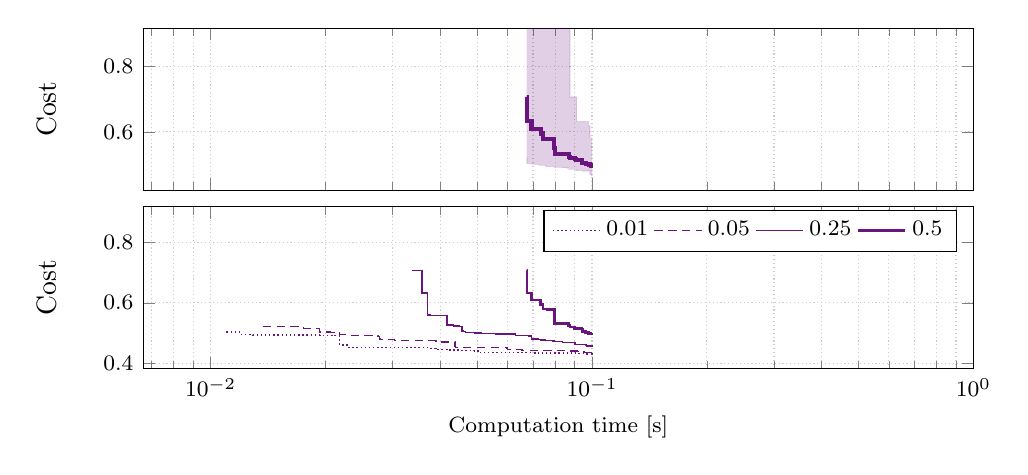
\begin{tikzpicture} [
  xscale=1,
  yscale=1
]
\begin{axis} [
  width=\textwidth,
  height=0.3\textwidth,
  at={(0cm, 0cm)},
  unbounded coords=jump,
  xtick align=inside,
  ytick align=inside,
  axis line style={solid, black},
  name=defaultInformedRRTstarMedianCostAxis,
  xmajorgrids,
  xminorgrids,
  ymajorgrids,
  major grid style={densely dotted, black!20},
  minor grid style={densely dotted, black!20},
  xmin=0.00665588,
  xmax=1,
  ymax=0.917277,
  xmode=log,
  xlabel={{\empty}},
  xlabel style={font=\footnotesize},
  xticklabel={{\empty}},
  xticklabel style={font=\footnotesize},
  ylabel={Cost},
  ylabel style={font=\footnotesize, text depth=0.0em, text height=0.5em},
  ylabel absolute,
  yticklabel style={font=\footnotesize}
]
\addplot [
  line width=0.5,
  color=pdtpurple,
  mark="none",
  const plot,
  name path={defaultInformedRRTstarMedianCostEvolutionUpperConfidence},
  fill opacity=0.2,
  draw opacity=0.1
] table [
  row sep=\\,
  col sep=&
]{
0.0674 & 2.75183\\
0.0874 & 2.75183\\
0.0875 & 0.70681\\
0.0911 & 0.70681\\
0.0912 & 0.632282\\
0.0979 & 0.632282\\
0.098 & 0.618009\\
0.0986 & 0.618009\\
0.0987 & 0.582012\\
0.0999 & 0.582012\\
0.1 & 0.582012\\
};

\addplot [
  line width=0.5,
  color=pdtpurple,
  mark="none",
  const plot,
  name path={defaultInformedRRTstarMedianCostEvolutionLowerConfidence},
  fill opacity=0.2,
  draw opacity=0.1
] table [
  row sep=\\,
  col sep=&
]{
0.0674 & 0.521862\\
0.0675 & 0.503083\\
0.0682 & 0.503083\\
0.0683 & 0.50254\\
0.0693 & 0.50254\\
0.0694 & 0.501393\\
0.0705 & 0.501393\\
0.0706 & 0.500978\\
0.0707 & 0.500392\\
0.0719 & 0.500392\\
0.072 & 0.500104\\
0.0723 & 0.500104\\
0.0724 & 0.499767\\
0.0727 & 0.499767\\
0.0728 & 0.497793\\
0.073 & 0.497793\\
0.0731 & 0.49779\\
0.0751 & 0.49779\\
0.0752 & 0.496947\\
0.0753 & 0.496347\\
0.0756 & 0.496347\\
0.0757 & 0.495435\\
0.0758 & 0.493925\\
0.0792 & 0.493925\\
0.0793 & 0.492915\\
0.0794 & 0.491447\\
0.081 & 0.491447\\
0.0811 & 0.491396\\
0.0831 & 0.491396\\
0.0832 & 0.490227\\
0.0859 & 0.490227\\
0.086 & 0.489312\\
0.0868 & 0.489312\\
0.0869 & 0.48537\\
0.0906 & 0.48537\\
0.0907 & 0.481489\\
0.0943 & 0.481489\\
0.0944 & 0.480687\\
0.0986 & 0.480687\\
0.0987 & 0.469659\\
0.0993 & 0.469659\\
0.0994 & 0.46715\\
0.0997 & 0.46715\\
0.0998 & 0.466826\\
0.0999 & 0.466826\\
0.1 & 0.466826\\
};

\addplot [
  line width=1,
  color=pdtpurple,
  mark=square*,
  mark size=2,
  const plot,
  fill opacity=0.2,
  draw opacity=0
] fill between [
  of =defaultInformedRRTstarMedianCostEvolutionUpperConfidence and defaultInformedRRTstarMedianCostEvolutionLowerConfidence
];
\addplot [
  line width=1.5,
  color=pdtpurple,
  mark="none",
  const plot,
  name path={defaultInformedRRTstarMedianCostEvolution}
] table [
  row sep=\\,
  col sep=&
]{
0.0001 & inf\\
0.0673 & inf\\
0.0674 & 0.70681\\
0.0675 & 0.632282\\
0.0693 & 0.632282\\
0.0694 & 0.609362\\
0.0733 & 0.609362\\
0.0734 & 0.595264\\
0.0743 & 0.595264\\
0.0744 & 0.579349\\
0.0763 & 0.579349\\
0.0764 & 0.576959\\
0.0796 & 0.576959\\
0.0797 & 0.551503\\
0.0798 & 0.551503\\
0.0799 & 0.532992\\
0.0868 & 0.532992\\
0.0869 & 0.525694\\
0.087 & 0.525694\\
0.0871 & 0.524031\\
0.0874 & 0.524031\\
0.0875 & 0.520627\\
0.0899 & 0.520627\\
0.09 & 0.515762\\
0.0905 & 0.515762\\
0.0906 & 0.515218\\
0.0937 & 0.515218\\
0.0938 & 0.513841\\
0.0942 & 0.513841\\
0.0943 & 0.504322\\
0.0962 & 0.504322\\
0.0963 & 0.500973\\
0.0979 & 0.500973\\
0.098 & 0.500019\\
0.0986 & 0.500019\\
0.0987 & 0.49779\\
0.0992 & 0.49779\\
0.0993 & 0.496798\\
0.0999 & 0.496798\\
0.1 & 0.496798\\
};

\end{axis}

\begin{axis} [
  width=\textwidth,
  height=0.3\textwidth,
  at={($(defaultInformedRRTstarMedianCostAxis.south) - (0.0em, 0.6em)$)},
  unbounded coords=jump,
  xtick align=inside,
  ytick align=inside,
  axis line style={solid, black},
  name=defaultInformedRRTstarCostPercentileEvolutionAxis,
  anchor=north,
  xmajorgrids,
  xminorgrids,
  ymajorgrids,
  major grid style={densely dotted, black!20},
  minor grid style={densely dotted, black!20},
  xmin=0.00665588,
  xmax=1,
  ymax=0.917277,
  xmode=log,
  xlabel={Computation time [s]},
  xlabel style={font=\footnotesize},
  xticklabel style={font=\footnotesize},
  ylabel={Cost},
  ylabel style={font=\footnotesize, text depth=0.0em, text height=0.5em},
  ylabel absolute,
  yticklabel style={font=\footnotesize},
  legend style={font=\footnotesize, legend cell align=left, legend columns=-1}
]
\addplot [
  line width=0.5,
  color=pdtpurple,
  mark="none",
  const plot,
  densely dotted,
  name path={defaultInformedRRTstarpercentile0.01CostEvolution}
] table [
  row sep=\\,
  col sep=&
]{
0.0001 & inf\\
0.0109 & inf\\
0.011 & 0.503633\\
0.0118 & 0.503633\\
0.0119 & 0.496347\\
0.0128 & 0.496347\\
0.0129 & 0.493719\\
0.0192 & 0.493719\\
0.0193 & 0.493002\\
0.0211 & 0.493002\\
0.0212 & 0.491447\\
0.0217 & 0.491447\\
0.0218 & 0.460868\\
0.0229 & 0.460868\\
0.023 & 0.452989\\
0.033 & 0.452989\\
0.0331 & 0.45233\\
0.0375 & 0.45233\\
0.0376 & 0.450059\\
0.0389 & 0.450059\\
0.039 & 0.445845\\
0.0416 & 0.445845\\
0.0417 & 0.444428\\
0.0425 & 0.444428\\
0.0426 & 0.444096\\
0.0448 & 0.444096\\
0.0449 & 0.443474\\
0.045 & 0.443081\\
0.0489 & 0.443081\\
0.049 & 0.442004\\
0.0491 & 0.44048\\
0.0502 & 0.44048\\
0.0503 & 0.43713\\
0.0504 & 0.435549\\
0.0707 & 0.435549\\
0.0708 & 0.435039\\
0.0709 & 0.434624\\
0.0904 & 0.434624\\
0.0905 & 0.432386\\
0.0932 & 0.432386\\
0.0933 & 0.432303\\
0.0934 & 0.432205\\
0.0959 & 0.432205\\
0.096 & 0.431963\\
0.0961 & 0.431475\\
0.0962 & 0.431422\\
0.0999 & 0.431422\\
0.1 & 0.431422\\
};
\addlegendentry{0.01}

\addplot [
  line width=0.5,
  color=pdtpurple,
  mark="none",
  const plot,
  densely dashed,
  name path={defaultInformedRRTstarpercentile0.05CostEvolution}
] table [
  row sep=\\,
  col sep=&
]{
0.0001 & inf\\
0.0136 & inf\\
0.0137 & 0.521862\\
0.0174 & 0.521862\\
0.0175 & 0.516163\\
0.0192 & 0.516163\\
0.0193 & 0.503633\\
0.0205 & 0.503633\\
0.0206 & 0.503083\\
0.0211 & 0.503083\\
0.0212 & 0.501277\\
0.0213 & 0.501277\\
0.0214 & 0.500392\\
0.0217 & 0.500392\\
0.0218 & 0.496347\\
0.0227 & 0.496347\\
0.0228 & 0.493719\\
0.0229 & 0.493002\\
0.0246 & 0.493002\\
0.0247 & 0.491447\\
0.0274 & 0.491447\\
0.0275 & 0.491124\\
0.0276 & 0.489312\\
0.0277 & 0.481363\\
0.0278 & 0.478612\\
0.0302 & 0.478612\\
0.0303 & 0.477033\\
0.0304 & 0.475802\\
0.0334 & 0.475802\\
0.0335 & 0.475523\\
0.0355 & 0.475523\\
0.0356 & 0.474954\\
0.0389 & 0.474954\\
0.039 & 0.472001\\
0.0402 & 0.472001\\
0.0403 & 0.471019\\
0.0404 & 0.47082\\
0.0435 & 0.47082\\
0.0436 & 0.47042\\
0.0437 & 0.456631\\
0.0438 & 0.45233\\
0.0598 & 0.45233\\
0.0599 & 0.448477\\
0.06 & 0.44521\\
0.0654 & 0.44521\\
0.0655 & 0.443506\\
0.0715 & 0.443506\\
0.0716 & 0.443081\\
0.0788 & 0.443081\\
0.0789 & 0.441743\\
0.0861 & 0.441743\\
0.0862 & 0.44123\\
0.0863 & 0.440622\\
0.0871 & 0.440622\\
0.0872 & 0.44056\\
0.0916 & 0.44056\\
0.0917 & 0.438553\\
0.0938 & 0.438553\\
0.0939 & 0.437887\\
0.094 & 0.437463\\
0.0953 & 0.437463\\
0.0954 & 0.436553\\
0.0993 & 0.436553\\
0.0994 & 0.436501\\
0.0996 & 0.436501\\
0.0997 & 0.435994\\
0.0998 & 0.434738\\
0.0999 & 0.434738\\
0.1 & 0.434738\\
};
\addlegendentry{0.05}

\addplot [
  line width=0.5,
  color=pdtpurple,
  mark="none",
  const plot,
  name path={defaultInformedRRTstarpercentile0.25CostEvolution}
] table [
  row sep=\\,
  col sep=&
]{
0.0001 & inf\\
0.0337 & inf\\
0.0338 & 0.70681\\
0.0357 & 0.70681\\
0.0358 & 0.632282\\
0.0369 & 0.632282\\
0.037 & 0.560338\\
0.0375 & 0.560338\\
0.0376 & 0.558857\\
0.0389 & 0.558857\\
0.039 & 0.557342\\
0.0415 & 0.557342\\
0.0416 & 0.55676\\
0.0417 & 0.526925\\
0.0433 & 0.526925\\
0.0434 & 0.524031\\
0.0449 & 0.524031\\
0.045 & 0.521862\\
0.0455 & 0.521862\\
0.0456 & 0.506736\\
0.0459 & 0.506736\\
0.046 & 0.50478\\
0.0465 & 0.50478\\
0.0466 & 0.503083\\
0.0473 & 0.503083\\
0.0474 & 0.501393\\
0.049 & 0.501393\\
0.0491 & 0.500392\\
0.051 & 0.500392\\
0.0511 & 0.499767\\
0.0521 & 0.499767\\
0.0522 & 0.49779\\
0.0558 & 0.49779\\
0.0559 & 0.497215\\
0.0596 & 0.497215\\
0.0597 & 0.496947\\
0.0628 & 0.496947\\
0.0629 & 0.496347\\
0.063 & 0.493076\\
0.0639 & 0.493076\\
0.064 & 0.491911\\
0.0668 & 0.491911\\
0.0669 & 0.491447\\
0.0674 & 0.491447\\
0.0675 & 0.491396\\
0.0682 & 0.491396\\
0.0683 & 0.490227\\
0.0693 & 0.490227\\
0.0694 & 0.488294\\
0.0695 & 0.480074\\
0.072 & 0.480074\\
0.0721 & 0.479293\\
0.0724 & 0.479293\\
0.0725 & 0.478174\\
0.0731 & 0.478174\\
0.0732 & 0.477248\\
0.0753 & 0.477248\\
0.0754 & 0.475408\\
0.0766 & 0.475408\\
0.0767 & 0.475385\\
0.0789 & 0.475385\\
0.079 & 0.474542\\
0.0794 & 0.474542\\
0.0795 & 0.473385\\
0.081 & 0.473385\\
0.0811 & 0.472611\\
0.0833 & 0.472611\\
0.0834 & 0.472278\\
0.0836 & 0.472278\\
0.0837 & 0.469659\\
0.0868 & 0.469659\\
0.0869 & 0.468998\\
0.0898 & 0.468998\\
0.0899 & 0.468396\\
0.09 & 0.467598\\
0.0901 & 0.467598\\
0.0902 & 0.465816\\
0.0903 & 0.464452\\
0.0904 & 0.463035\\
0.0906 & 0.463035\\
0.0907 & 0.462192\\
0.0964 & 0.462192\\
0.0965 & 0.4591\\
0.0966 & 0.458005\\
0.0974 & 0.458005\\
0.0975 & 0.4575\\
0.099 & 0.4575\\
0.0991 & 0.457017\\
0.0993 & 0.457017\\
0.0994 & 0.45696\\
0.0999 & 0.45696\\
0.1 & 0.455895\\
};
\addlegendentry{0.25}

\addplot [
  line width=1,
  color=pdtpurple,
  mark="none",
  const plot,
  name path={defaultInformedRRTstarpercentile0.5CostEvolution}
] table [
  row sep=\\,
  col sep=&
]{
0.0001 & inf\\
0.0673 & inf\\
0.0674 & 0.70681\\
0.0675 & 0.632282\\
0.0693 & 0.632282\\
0.0694 & 0.609362\\
0.0733 & 0.609362\\
0.0734 & 0.595264\\
0.0743 & 0.595264\\
0.0744 & 0.579349\\
0.0763 & 0.579349\\
0.0764 & 0.576959\\
0.0796 & 0.576959\\
0.0797 & 0.551503\\
0.0798 & 0.551503\\
0.0799 & 0.532992\\
0.0868 & 0.532992\\
0.0869 & 0.525694\\
0.087 & 0.525694\\
0.0871 & 0.524031\\
0.0874 & 0.524031\\
0.0875 & 0.520627\\
0.0899 & 0.520627\\
0.09 & 0.515762\\
0.0905 & 0.515762\\
0.0906 & 0.515218\\
0.0937 & 0.515218\\
0.0938 & 0.513841\\
0.0942 & 0.513841\\
0.0943 & 0.504322\\
0.0962 & 0.504322\\
0.0963 & 0.500973\\
0.0979 & 0.500973\\
0.098 & 0.500019\\
0.0986 & 0.500019\\
0.0987 & 0.49779\\
0.0992 & 0.49779\\
0.0993 & 0.496798\\
0.0999 & 0.496798\\
0.1 & 0.496798\\
};
\addlegendentry{0.5}

\addplot [
  line width=0.5,
  color=pdtpurple,
  mark="none",
  const plot,
  name path={defaultInformedRRTstarpercentile0.75CostEvolution}
] table [
  row sep=\\,
  col sep=&
]{
0.0001 & inf\\
0.0999 & inf\\
0.1 & inf\\
};
\addlegendentry{0.75}

\addplot [
  line width=0.5,
  color=pdtpurple,
  mark="none",
  const plot,
  densely dashed,
  name path={defaultInformedRRTstarpercentile0.95CostEvolution}
] table [
  row sep=\\,
  col sep=&
]{
0.0001 & inf\\
0.0999 & inf\\
0.1 & inf\\
};
\addlegendentry{0.95}

\addplot [
  line width=0.5,
  color=pdtpurple,
  mark="none",
  const plot,
  densely dotted,
  name path={defaultInformedRRTstarpercentile0.99CostEvolution}
] table [
  row sep=\\,
  col sep=&
]{
0.0001 & inf\\
0.0999 & inf\\
0.1 & inf\\
};
\addlegendentry{0.99}

\end{axis}

\end{tikzpicture}%
\captionof{figure}{\footnotesize \textbf{Top:} Median cost evolution of Informed RRT* with a nonparametric 99\% confidence interval. \textbf{Bottom:} Seven percentiles of the cost evolution of Informed RRT*.}\end{center}

\pagebreak
\section{AIT*}\label{sec:defaultAITstar}
\subsection{Initial Solutions}\label{sec:defaultAITstar-initial-solution}
\begin{center}
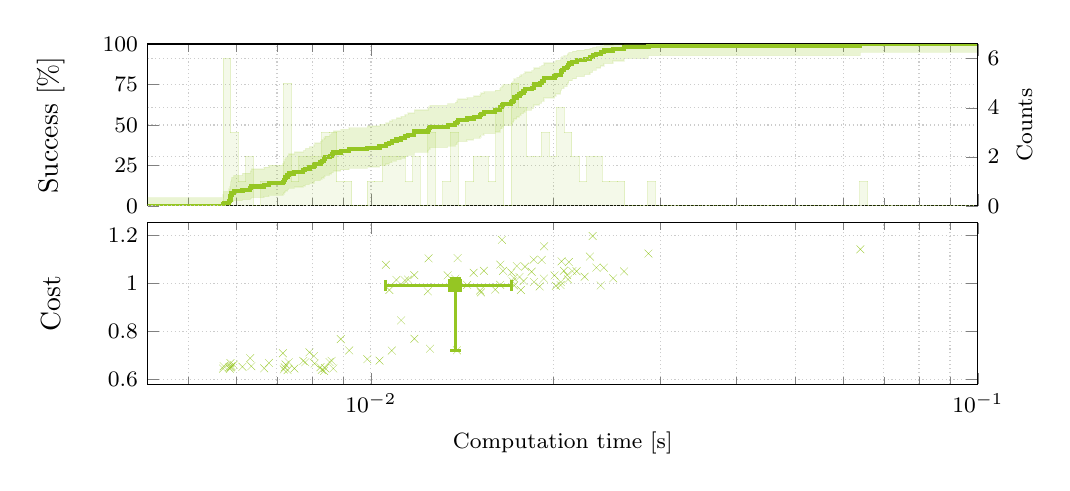
\begin{tikzpicture} [
  xscale=1,
  yscale=1
]
\begin{axis} [
  width=\textwidth,
  height=0.3\textwidth,
  at={(0cm, 0cm)},
  unbounded coords=jump,
  xtick align=inside,
  ytick align=inside,
  axis line style={solid, black},
  name=SuccessAxis,
  xmajorgrids,
  xminorgrids,
  ymajorgrids,
  major grid style={densely dotted, black!20},
  minor grid style={densely dotted, black!20},
  xmin=0.00570601,
  xmax=0.1,
  enlarge x limits=lower,
  ymin=0,
  ymax=100,
  xmode=log,
  xlabel={{\empty}},
  xlabel style={font=\footnotesize},
  xticklabel={{\empty}},
  xticklabel style={font=\footnotesize},
  ylabel={Success [\%]},
  ylabel style={font=\footnotesize, text depth=0.0em, text height=0.5em},
  ylabel absolute,
  ytick={0,25,50,75,100},
 ytick pos={left},
  yticklabel style={font=\footnotesize}
]
\addplot [
  line width=0.5,
  color=pdtlightgreen,
  mark="none",
  const plot,
  name path={defaultAITstarSuccessUpperConfidence},
  fill opacity=0.2,
  draw opacity=0.1
] table [
  row sep=\\,
  col sep=&
]{
1e-09 & 5.1604\\
0.00570601 & 7.19577\\
0.00572016 & 8.94307\\
0.00583449 & 10.5481\\
0.0058551 & 12.0633\\
0.00586758 & 13.5145\\
0.00586919 & 14.9169\\
0.00588531 & 16.2803\\
0.00589186 & 17.6114\\
0.00594105 & 18.9152\\
0.00614074 & 20.1954\\
0.00632617 & 21.4547\\
0.00635233 & 22.6955\\
0.00666972 & 23.9196\\
0.00679166 & 25.1285\\
0.0071604 & 26.3235\\
0.00718568 & 27.5057\\
0.00721124 & 28.676\\
0.00723253 & 29.8351\\
0.00728822 & 30.9838\\
0.00732123 & 32.1226\\
0.00748032 & 33.2522\\
0.00773605 & 34.3729\\
0.00779485 & 35.4851\\
0.00792104 & 36.5893\\
0.00805323 & 37.6857\\
0.00807747 & 38.7747\\
0.00825625 & 39.8566\\
0.00829883 & 40.9315\\
0.00837205 & 41.9997\\
0.00840076 & 43.0614\\
0.00854802 & 44.1167\\
0.00861402 & 45.1659\\
0.00866793 & 46.2091\\
0.00891837 & 47.2464\\
0.00920707 & 48.2779\\
0.00986525 & 49.3038\\
0.0103308 & 50.3241\\
0.010583 & 51.339\\
0.0107237 & 52.3485\\
0.0108263 & 53.3527\\
0.0110168 & 54.3517\\
0.0112149 & 55.3454\\
0.0113757 & 56.3341\\
0.0115145 & 57.3177\\
0.0117879 & 58.2962\\
0.011793 & 59.2697\\
0.0124089 & 60.2382\\
0.0124461 & 61.2017\\
0.0125126 & 62.1603\\
0.0133792 & 63.1139\\
0.0137698 & 64.0625\\
0.0138588 & 65.0062\\
0.0138943 & 65.9449\\
0.0144061 & 66.8786\\
0.0147661 & 67.8073\\
0.0151349 & 68.7309\\
0.0151813 & 69.6495\\
0.0153486 & 70.5629\\
0.0160255 & 71.4712\\
0.0163294 & 72.3742\\
0.0163374 & 73.272\\
0.016438 & 74.1644\\
0.0165099 & 75.0513\\
0.0170362 & 75.9327\\
0.0171145 & 76.8085\\
0.0171938 & 77.6785\\
0.0172156 & 78.5426\\
0.0173904 & 79.4008\\
0.0175692 & 80.2528\\
0.0176625 & 81.0985\\
0.0178457 & 81.9378\\
0.0179438 & 82.7703\\
0.0184035 & 83.596\\
0.0185446 & 84.4145\\
0.0185669 & 85.2256\\
0.0189686 & 86.0291\\
0.0191163 & 86.8245\\
0.019278 & 87.6116\\
0.0192929 & 88.3899\\
0.0200707 & 89.1589\\
0.0201723 & 89.9183\\
0.0205348 & 90.6673\\
0.0205484 & 91.4053\\
0.0206144 & 92.1315\\
0.0207943 & 92.8452\\
0.0210563 & 93.5451\\
0.0211279 & 94.2303\\
0.0211825 & 94.8991\\
0.021476 & 95.5498\\
0.0218223 & 96.1804\\
0.0224939 & 96.7882\\
0.0229585 & 97.3699\\
0.0231919 & 97.921\\
0.0235216 & 98.4357\\
0.023915 & 98.906\\
0.0241937 & 99.3198\\
0.0250701 & 99.6593\\
0.0261297 & 99.896\\
0.028661 & 99.995\\
0.0640388 & 100\\
0.109124 & 100\\
};

\addplot [
  line width=0.5,
  color=pdtlightgreen,
  mark="none",
  const plot,
  name path={defaultAITstarSuccessLowerConfidence},
  fill opacity=0.2,
  draw opacity=0.1
] table [
  row sep=\\,
  col sep=&
]{
1e-09 & 0\\
0.00570601 & 0.00501242\\
0.00572016 & 0.103962\\
0.00583449 & 0.340707\\
0.0058551 & 0.680169\\
0.00586758 & 1.09403\\
0.00586919 & 1.56425\\
0.00588531 & 2.07899\\
0.00589186 & 2.63012\\
0.00594105 & 3.21176\\
0.00614074 & 3.81957\\
0.00632617 & 4.45017\\
0.00635233 & 5.10094\\
0.00666972 & 5.76975\\
0.00679166 & 6.45486\\
0.0071604 & 7.15483\\
0.00718568 & 7.86846\\
0.00721124 & 8.59473\\
0.00723253 & 9.33274\\
0.00728822 & 10.0817\\
0.00732123 & 10.8411\\
0.00748032 & 11.6101\\
0.00773605 & 12.3884\\
0.00779485 & 13.1755\\
0.00792104 & 13.9709\\
0.00805323 & 14.7744\\
0.00807747 & 15.5855\\
0.00825625 & 16.404\\
0.00829883 & 17.2297\\
0.00837205 & 18.0622\\
0.00840076 & 18.9015\\
0.00854802 & 19.7472\\
0.00861402 & 20.5992\\
0.00866793 & 21.4574\\
0.00891837 & 22.3215\\
0.00920707 & 23.1915\\
0.00986525 & 24.0673\\
0.0103308 & 24.9487\\
0.010583 & 25.8356\\
0.0107237 & 26.728\\
0.0108263 & 27.6258\\
0.0110168 & 28.5288\\
0.0112149 & 29.4371\\
0.0113757 & 30.3505\\
0.0115145 & 31.2691\\
0.0117879 & 32.1927\\
0.011793 & 33.1214\\
0.0124089 & 34.0551\\
0.0124461 & 34.9938\\
0.0125126 & 35.9375\\
0.0133792 & 36.8861\\
0.0137698 & 37.8397\\
0.0138588 & 38.7983\\
0.0138943 & 39.7618\\
0.0144061 & 40.7303\\
0.0147661 & 41.7038\\
0.0151349 & 42.6823\\
0.0151813 & 43.6659\\
0.0153486 & 44.6546\\
0.0160255 & 45.6483\\
0.0163294 & 46.6473\\
0.0163374 & 47.6515\\
0.016438 & 48.661\\
0.0165099 & 49.6759\\
0.0170362 & 50.6962\\
0.0171145 & 51.7221\\
0.0171938 & 52.7536\\
0.0172156 & 53.7909\\
0.0173904 & 54.8341\\
0.0175692 & 55.8833\\
0.0176625 & 56.9386\\
0.0178457 & 58.0003\\
0.0179438 & 59.0685\\
0.0184035 & 60.1434\\
0.0185446 & 61.2253\\
0.0185669 & 62.3143\\
0.0189686 & 63.4107\\
0.0191163 & 64.5149\\
0.019278 & 65.6271\\
0.0192929 & 66.7478\\
0.0200707 & 67.8774\\
0.0201723 & 69.0162\\
0.0205348 & 70.1649\\
0.0205484 & 71.324\\
0.0206144 & 72.4943\\
0.0207943 & 73.6765\\
0.0210563 & 74.8715\\
0.0211279 & 76.0804\\
0.0211825 & 77.3045\\
0.021476 & 78.5453\\
0.0218223 & 79.8046\\
0.0224939 & 81.0848\\
0.0229585 & 82.3886\\
0.0231919 & 83.7197\\
0.0235216 & 85.0831\\
0.023915 & 86.4855\\
0.0241937 & 87.9367\\
0.0250701 & 89.4519\\
0.0261297 & 91.0569\\
0.028661 & 92.8042\\
0.0640388 & 94.8396\\
0.109124 & 94.8396\\
};

\addplot [
  line width=1,
  color=pdtlightgreen,
  mark=square*,
  mark size=2,
  const plot,
  fill opacity=0.2,
  draw opacity=0
] fill between [
  of =defaultAITstarSuccessUpperConfidence and defaultAITstarSuccessLowerConfidence
];
\addplot [
  line width=1.5,
  color=pdtlightgreen,
  mark="none",
  const plot,
  name path={defaultAITstarSuccess}
] table [
  row sep=\\,
  col sep=&
]{
1e-09 & 0\\
0.00570601 & 1\\
0.00572016 & 2\\
0.00583449 & 3\\
0.0058551 & 4\\
0.00586758 & 5\\
0.00586919 & 6\\
0.00588531 & 7\\
0.00589186 & 8\\
0.00594105 & 9\\
0.00614074 & 10\\
0.00632617 & 11\\
0.00635233 & 12\\
0.00666972 & 13\\
0.00679166 & 14\\
0.0071604 & 15\\
0.00718568 & 16\\
0.00721124 & 17\\
0.00723253 & 18\\
0.00728822 & 19\\
0.00732123 & 20\\
0.00748032 & 21\\
0.00773605 & 22\\
0.00779485 & 23\\
0.00792104 & 24\\
0.00805323 & 25\\
0.00807747 & 26\\
0.00825625 & 27\\
0.00829883 & 28\\
0.00837205 & 29\\
0.00840076 & 30\\
0.00854802 & 31\\
0.00861402 & 32\\
0.00866793 & 33\\
0.00891837 & 34\\
0.00920707 & 35\\
0.00986525 & 36\\
0.0103308 & 37\\
0.010583 & 38\\
0.0107237 & 39\\
0.0108263 & 40\\
0.0110168 & 41\\
0.0112149 & 42\\
0.0113757 & 43\\
0.0115145 & 44\\
0.0117879 & 45\\
0.011793 & 46\\
0.0124089 & 47\\
0.0124461 & 48\\
0.0125126 & 49\\
0.0133792 & 50\\
0.0137698 & 51\\
0.0138588 & 52\\
0.0138943 & 53\\
0.0144061 & 54\\
0.0147661 & 55\\
0.0151349 & 56\\
0.0151813 & 57\\
0.0153486 & 58\\
0.0160255 & 59\\
0.0163294 & 60\\
0.0163374 & 61\\
0.016438 & 62\\
0.0165099 & 63\\
0.0170362 & 64\\
0.0171145 & 65\\
0.0171938 & 66\\
0.0172156 & 67\\
0.0173904 & 68\\
0.0175692 & 69\\
0.0176625 & 70\\
0.0178457 & 71\\
0.0179438 & 72\\
0.0184035 & 73\\
0.0185446 & 74\\
0.0185669 & 75\\
0.0189686 & 76\\
0.0191163 & 77\\
0.019278 & 78\\
0.0192929 & 79\\
0.0200707 & 80\\
0.0201723 & 81\\
0.0205348 & 82\\
0.0205484 & 83\\
0.0206144 & 84\\
0.0207943 & 85\\
0.0210563 & 86\\
0.0211279 & 87\\
0.0211825 & 88\\
0.021476 & 89\\
0.0218223 & 90\\
0.0224939 & 91\\
0.0229585 & 92\\
0.0231919 & 93\\
0.0235216 & 94\\
0.023915 & 95\\
0.0241937 & 96\\
0.0250701 & 97\\
0.0261297 & 98\\
0.028661 & 99\\
0.0640388 & 100\\
0.109124 & 100\\
};

\end{axis}

\begin{axis} [
  width=\textwidth,
  height=0.3\textwidth,
  at={(0cm, 0cm)},
  unbounded coords=jump,
  xtick align=inside,
  ytick align=inside,
  axis line style={solid, black},
  name=defaultAITstarISDPA,
  xmajorgrids,
  xminorgrids,
  ymajorgrids,
  major grid style={densely dotted, black!20},
  minor grid style={densely dotted, black!20},
  xmin=0.00570601,
  xmax=0.1,
  enlarge x limits=lower,
  ymin=0,
  ymax=6,
  enlarge y limits=upper,
  xmode=log,
  axis x line=none,
  axis y line*=right,
  xlabel={Computation time [s]},
  xlabel style={font=\footnotesize},
  xtick={{\empty}},
  xticklabel={{\empty}},
  xticklabel style={font=\footnotesize},
  ylabel={Counts},
  ylabel style={font=\footnotesize, text depth=0.0em, text height=0.5em},
  yticklabel style={font=\footnotesize}
]
\addplot [
  line width=0,
  color=pdtlightgreen,
  mark="none",
  const plot,
  name path={defaultAITstarInitialSolutionDurationHistogram},
  fill=pdtlightgreen,
  fill opacity=0.1,
  draw opacity=0.2
] table [
  row sep=\\,
  col sep=&
]{
0.00570601 & 0\\
0.00570601 & 6\\
0.00587252 & 3\\
0.0060439 & 1\\
0.00622027 & 2\\
0.00640179 & 0\\
0.00658861 & 1\\
0.00678089 & 1\\
0.00697877 & 1\\
0.00718243 & 5\\
0.00739203 & 1\\
0.00760774 & 2\\
0.00782975 & 2\\
0.00805825 & 2\\
0.0082934 & 3\\
0.00853543 & 3\\
0.00878451 & 1\\
0.00904086 & 1\\
0.0093047 & 0\\
0.00957623 & 0\\
0.00985569 & 1\\
0.0101433 & 1\\
0.0104393 & 2\\
0.0107439 & 2\\
0.0110575 & 2\\
0.0113802 & 1\\
0.0117123 & 2\\
0.0120541 & 0\\
0.0124058 & 3\\
0.0127679 & 0\\
0.0131405 & 1\\
0.0135239 & 3\\
0.0139186 & 0\\
0.0143248 & 1\\
0.0147428 & 2\\
0.015173 & 2\\
0.0156158 & 1\\
0.0160715 & 4\\
0.0165405 & 0\\
0.0170232 & 5\\
0.01752 & 4\\
0.0180313 & 2\\
0.0185575 & 2\\
0.019099 & 3\\
0.0196564 & 2\\
0.02023 & 4\\
0.0208203 & 3\\
0.0214279 & 2\\
0.0220532 & 1\\
0.0226968 & 2\\
0.0233592 & 2\\
0.0240408 & 1\\
0.0247424 & 1\\
0.0254644 & 1\\
0.0262076 & 0\\
0.0269724 & 0\\
0.0277595 & 0\\
0.0285696 & 1\\
0.0294033 & 0\\
0.0302613 & 0\\
0.0311444 & 0\\
0.0320533 & 0\\
0.0329887 & 0\\
0.0339514 & 0\\
0.0349422 & 0\\
0.0359619 & 0\\
0.0370113 & 0\\
0.0380914 & 0\\
0.039203 & 0\\
0.040347 & 0\\
0.0415245 & 0\\
0.0427362 & 0\\
0.0439834 & 0\\
0.0452669 & 0\\
0.0465879 & 0\\
0.0479475 & 0\\
0.0493467 & 0\\
0.0507867 & 0\\
0.0522688 & 0\\
0.0537941 & 0\\
0.055364 & 0\\
0.0569796 & 0\\
0.0586424 & 0\\
0.0603538 & 0\\
0.062115 & 0\\
0.0639277 & 1\\
0.0657933 & 0\\
0.0677133 & 0\\
0.0696893 & 0\\
0.071723 & 0\\
0.073816 & 0\\
0.0759702 & 0\\
0.0781872 & 0\\
0.0804688 & 0\\
0.0828171 & 0\\
0.0852339 & 0\\
0.0877213 & 0\\
0.0902812 & 0\\
0.0929158 & 0\\
0.0956273 & 0\\
0.0984179 & 0\\
0.0984179 & 0\\
};

\end{axis}

\begin{axis} [
  width=\textwidth,
  height=0.3\textwidth,
  at={($(SuccessAxis.south) - (0.0em, 0.6em)$)},
  unbounded coords=jump,
  xtick align=inside,
  ytick align=inside,
  axis line style={solid, black},
  name=defaultAITstarInitialSolutionScatterAxis,
  anchor=north,
  xmajorgrids,
  xminorgrids,
  ymajorgrids,
  major grid style={densely dotted, black!20},
  minor grid style={densely dotted, black!20},
  xmin=0.00570601,
  xmax=0.1,
  enlarge x limits=lower,
  xmode=log,
  xlabel={Computation time [s]},
  xlabel style={font=\footnotesize},
  xticklabel style={font=\footnotesize},
  ylabel={Cost},
  ylabel style={font=\footnotesize, text depth=0.0em, text height=0.5em},
  ylabel absolute,
  yticklabel style={font=\footnotesize}
]
\addplot [
  line width=0.1,
  color=pdtlightgreen,
  mark=x,
  mark size=2,
  only marks,
  name path={defaultAITstarInitialSolutionScatterPlotlineWidth}
] table [
  row sep=\\,
  col sep=&
]{
0.0250701 & 1.02179\\
0.0206144 & 1.09293\\
0.0261297 & 1.05057\\
0.00732123 & 0.670615\\
0.0205348 & 0.993721\\
0.0103308 & 0.677418\\
0.0640388 & 1.14342\\
0.00614074 & 0.651398\\
0.010583 & 1.07851\\
0.0151813 & 0.963137\\
0.0138588 & 0.720656\\
0.00721124 & 0.649059\\
0.0185669 & 1.0064\\
0.0124089 & 0.96738\\
0.00679166 & 0.667794\\
0.00594105 & 0.660506\\
0.0235216 & 1.06673\\
0.0178457 & 1.01032\\
0.0163294 & 0.994519\\
0.00718568 & 0.640637\\
0.0151349 & 0.970868\\
0.0192929 & 1.15571\\
0.00589186 & 0.654858\\
0.0125126 & 0.727209\\
0.00807747 & 0.665167\\
0.0163374 & 1.07894\\
0.0110168 & 1.01506\\
0.00837205 & 0.634335\\
0.0231919 & 1.19889\\
0.0173904 & 1.07327\\
0.0133792 & 1.03452\\
0.00854802 & 0.671538\\
0.00572016 & 0.654293\\
0.0218223 & 1.05163\\
0.0160255 & 0.974809\\
0.00825625 & 0.64997\\
0.00829883 & 0.638767\\
0.00632617 & 0.687642\\
0.00805323 & 0.696365\\
0.0191163 & 1.09871\\
0.00840076 & 0.646042\\
0.0144061 & 0.994279\\
0.00866793 & 0.644685\\
0.0115145 & 1.01672\\
0.0112149 & 0.845945\\
0.00586758 & 0.648159\\
0.0241937 & 1.06624\\
0.0113757 & 1.01305\\
0.0179438 & 1.07097\\
0.0165099 & 1.05319\\
0.00586919 & 0.66684\\
0.0071604 & 0.7083\\
0.0117879 & 1.0352\\
0.016438 & 1.18288\\
0.0058551 & 0.642958\\
0.0200707 & 1.03409\\
0.0175692 & 1.02738\\
0.0108263 & 0.719511\\
0.00570601 & 0.644372\\
0.00773605 & 0.67606\\
0.0176625 & 0.972947\\
0.0224939 & 1.02852\\
0.00891837 & 0.767222\\
0.023915 & 0.992022\\
0.00588531 & 0.651438\\
0.00792104 & 0.712349\\
0.0205484 & 1.00633\\
0.00723253 & 0.66141\\
0.00635233 & 0.654218\\
0.0172156 & 0.991939\\
0.00748032 & 0.644439\\
0.0229585 & 1.11301\\
0.0138943 & 1.10643\\
0.011793 & 0.768912\\
0.0189686 & 0.987899\\
0.0124461 & 1.10562\\
0.0207943 & 1.05378\\
0.0184035 & 1.04937\\
0.0137698 & 1.02019\\
0.028661 & 1.12551\\
0.0211825 & 1.08999\\
0.00728822 & 0.637834\\
0.00779485 & 0.670774\\
0.0107237 & 0.973075\\
0.0201723 & 0.99067\\
0.00666972 & 0.64533\\
0.0171145 & 1.00931\\
0.019278 & 1.02058\\
0.0210563 & 1.03529\\
0.00920707 & 0.720006\\
0.00861402 & 0.676343\\
0.0170362 & 1.04646\\
0.0171938 & 1.02328\\
0.021476 & 1.052\\
0.0185446 & 1.09974\\
0.00986525 & 0.68347\\
0.0153486 & 1.05347\\
0.0147661 & 1.04508\\
0.00583449 & 0.648836\\
0.0211279 & 1.0174\\
};

\addplot [
  line width=1,
  color=pdtlightgreen,
  mark=square*,
  mark size=2,
  only marks,
  const plot,
  name path={defaultAITstarMedianInitialSolution}
] table [
  row sep=\\,
  col sep=&
]{
0.0137698 & 0.991939\\
};

\addplot [
  line width=1,
  color=pdtlightgreen,
  mark=|,
  mark size=2,
  const plot,
  name path={defaultAITstarMedianInitialSolutionDurationConfidenceInterval}
] table [
  row sep=\\,
  col sep=&
]{
0.010583 & 0.991939\\
0.0170362 & 0.991939\\
};

\addplot [
  line width=1,
  color=pdtlightgreen,
  mark=-,
  mark size=2,
  const plot,
  name path={defaultAITstarMedianInitialSolutionDurationConfidenceInterval}
] table [
  row sep=\\,
  col sep=&
]{
0.0137698 & 0.720656\\
0.0137698 & 1.02019\\
};

\end{axis}

\end{tikzpicture}%
\captionof{figure}{\footnotesize \textbf{Top:} Histogram and associated empirical distribution function (EDF) of AIT* with a Clopper-Pearson (nonparametric) 99\% confidence interval for the underlying CDF. \textbf{Bottom:} All initial solutions of AIT* and their median with a nonparametric 99\% confidence interval.}
\end{center}
\subsection{Cost Evolution}\label{sec:defaultAITstar-cost-evolution}
\begin{center}
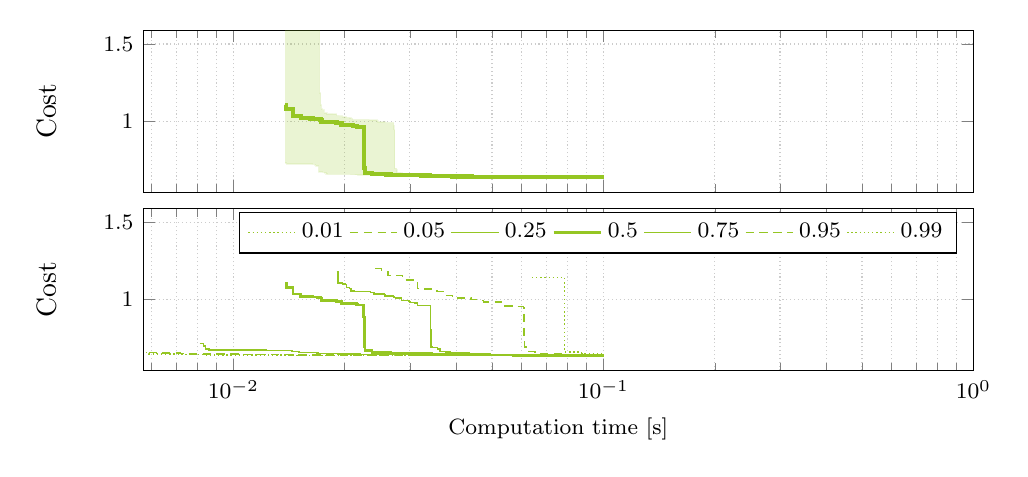
\begin{tikzpicture} [
  xscale=1,
  yscale=1
]
\begin{axis} [
  width=\textwidth,
  height=0.3\textwidth,
  at={(0cm, 0cm)},
  unbounded coords=jump,
  xtick align=inside,
  ytick align=inside,
  axis line style={solid, black},
  name=defaultAITstarMedianCostAxis,
  xmajorgrids,
  xminorgrids,
  ymajorgrids,
  major grid style={densely dotted, black!20},
  minor grid style={densely dotted, black!20},
  xmin=0.00570601,
  xmax=1,
  ymax=1.58998,
  xmode=log,
  xlabel={{\empty}},
  xlabel style={font=\footnotesize},
  xticklabel={{\empty}},
  xticklabel style={font=\footnotesize},
  ylabel={Cost},
  ylabel style={font=\footnotesize, text depth=0.0em, text height=0.5em},
  ylabel absolute,
  yticklabel style={font=\footnotesize}
]
\addplot [
  line width=0.5,
  color=pdtlightgreen,
  mark="none",
  const plot,
  name path={defaultAITstarMedianCostEvolutionUpperConfidence},
  fill opacity=0.2,
  draw opacity=0.1
] table [
  row sep=\\,
  col sep=&
]{
0.0138 & 4.76994\\
0.017 & 4.76994\\
0.0171 & 1.18288\\
0.0172 & 1.10562\\
0.0173 & 1.07894\\
0.0174 & 1.07327\\
0.0175 & 1.07327\\
0.0176 & 1.05347\\
0.0177 & 1.05319\\
0.0178 & 1.05319\\
0.0179 & 1.04646\\
0.0185 & 1.04646\\
0.0186 & 1.04508\\
0.0189 & 1.04508\\
0.019 & 1.0352\\
0.0192 & 1.0352\\
0.0193 & 1.03452\\
0.0196 & 1.03452\\
0.0197 & 1.02738\\
0.0201 & 1.02738\\
0.0202 & 1.02328\\
0.0205 & 1.02328\\
0.0206 & 1.02019\\
0.0207 & 1.02019\\
0.0208 & 1.01672\\
0.0209 & 1.01672\\
0.021 & 1.01032\\
0.0215 & 1.01032\\
0.0216 & 1.00931\\
0.0232 & 1.00931\\
0.0233 & 1.0064\\
0.0239 & 1.0064\\
0.024 & 1.00633\\
0.0244 & 1.00633\\
0.0245 & 1.00002\\
0.0246 & 0.994519\\
0.025 & 0.994519\\
0.0251 & 0.993721\\
0.0256 & 0.993721\\
0.0257 & 0.99067\\
0.0258 & 0.989364\\
0.027 & 0.989364\\
0.0271 & 0.972947\\
0.0272 & 0.945353\\
0.0273 & 0.693508\\
0.0275 & 0.693508\\
0.0276 & 0.682454\\
0.0277 & 0.665486\\
0.0283 & 0.665486\\
0.0284 & 0.662318\\
0.0285 & 0.662318\\
0.0286 & 0.661736\\
0.0288 & 0.661736\\
0.0289 & 0.657026\\
0.029 & 0.657026\\
0.0291 & 0.656024\\
0.0292 & 0.656024\\
0.0293 & 0.655803\\
0.0298 & 0.655803\\
0.0299 & 0.655339\\
0.0319 & 0.655339\\
0.032 & 0.654746\\
0.0321 & 0.654746\\
0.0322 & 0.653887\\
0.0326 & 0.653887\\
0.0327 & 0.653264\\
0.0328 & 0.653135\\
0.0329 & 0.652032\\
0.0339 & 0.652032\\
0.034 & 0.651574\\
0.0343 & 0.651574\\
0.0344 & 0.650132\\
0.0355 & 0.650132\\
0.0356 & 0.649267\\
0.0358 & 0.649267\\
0.0359 & 0.649103\\
0.0363 & 0.649103\\
0.0364 & 0.649003\\
0.0367 & 0.649003\\
0.0368 & 0.648514\\
0.0373 & 0.648514\\
0.0374 & 0.648348\\
0.0378 & 0.648348\\
0.0379 & 0.646694\\
0.038 & 0.646694\\
0.0381 & 0.645913\\
0.0384 & 0.645913\\
0.0385 & 0.645617\\
0.0393 & 0.645617\\
0.0394 & 0.645527\\
0.0401 & 0.645527\\
0.0402 & 0.645383\\
0.0403 & 0.645233\\
0.0404 & 0.64453\\
0.0406 & 0.64453\\
0.0407 & 0.644294\\
0.0418 & 0.644294\\
0.0419 & 0.644022\\
0.043 & 0.644022\\
0.0431 & 0.643664\\
0.0432 & 0.643484\\
0.0433 & 0.643142\\
0.0434 & 0.64223\\
0.0437 & 0.64223\\
0.0438 & 0.642081\\
0.0439 & 0.642081\\
0.044 & 0.641893\\
0.0441 & 0.641581\\
0.045 & 0.641581\\
0.0451 & 0.641553\\
0.0454 & 0.641553\\
0.0455 & 0.641196\\
0.0456 & 0.641196\\
0.0457 & 0.641181\\
0.0458 & 0.641091\\
0.0463 & 0.641091\\
0.0464 & 0.641073\\
0.0471 & 0.641073\\
0.0472 & 0.640831\\
0.0477 & 0.640831\\
0.0478 & 0.640677\\
0.048 & 0.640677\\
0.0481 & 0.64042\\
0.0494 & 0.64042\\
0.0495 & 0.640331\\
0.0499 & 0.640331\\
0.05 & 0.640255\\
0.0501 & 0.640211\\
0.0514 & 0.640211\\
0.0515 & 0.640103\\
0.053 & 0.640103\\
0.0531 & 0.640103\\
0.0532 & 0.639869\\
0.0543 & 0.639869\\
0.0544 & 0.639853\\
0.0545 & 0.63968\\
0.0546 & 0.63957\\
0.0549 & 0.63957\\
0.055 & 0.639557\\
0.0551 & 0.639393\\
0.0552 & 0.639139\\
0.0555 & 0.639139\\
0.0556 & 0.638959\\
0.0557 & 0.638959\\
0.0558 & 0.638897\\
0.0567 & 0.638897\\
0.0568 & 0.638896\\
0.0569 & 0.638689\\
0.0572 & 0.638689\\
0.0573 & 0.638632\\
0.0574 & 0.638596\\
0.0577 & 0.638596\\
0.0578 & 0.638576\\
0.0598 & 0.638576\\
0.0599 & 0.638534\\
0.0604 & 0.638534\\
0.0605 & 0.638473\\
0.0606 & 0.638473\\
0.0607 & 0.638423\\
0.0609 & 0.638423\\
0.061 & 0.638421\\
0.062 & 0.638421\\
0.0621 & 0.638345\\
0.0622 & 0.638293\\
0.0624 & 0.638293\\
0.0625 & 0.638242\\
0.0631 & 0.638242\\
0.0632 & 0.638217\\
0.0635 & 0.638217\\
0.0636 & 0.638182\\
0.0637 & 0.638182\\
0.0638 & 0.63812\\
0.0639 & 0.638037\\
0.0667 & 0.638037\\
0.0668 & 0.637975\\
0.0669 & 0.637884\\
0.0677 & 0.637884\\
0.0678 & 0.637872\\
0.0679 & 0.63771\\
0.0697 & 0.63771\\
0.0698 & 0.637684\\
0.0699 & 0.637652\\
0.07 & 0.637626\\
0.0713 & 0.637626\\
0.0714 & 0.637613\\
0.0719 & 0.637613\\
0.072 & 0.637612\\
0.0735 & 0.637612\\
0.0736 & 0.637604\\
0.0757 & 0.637604\\
0.0758 & 0.637503\\
0.0759 & 0.637371\\
0.0772 & 0.637371\\
0.0773 & 0.637328\\
0.0785 & 0.637328\\
0.0786 & 0.637177\\
0.0795 & 0.637177\\
0.0796 & 0.637026\\
0.08 & 0.637026\\
0.0801 & 0.636931\\
0.0829 & 0.636931\\
0.083 & 0.636915\\
0.0845 & 0.636915\\
0.0846 & 0.636897\\
0.0847 & 0.63687\\
0.0848 & 0.63687\\
0.0849 & 0.636827\\
0.0874 & 0.636827\\
0.0875 & 0.636795\\
0.0876 & 0.636594\\
0.0885 & 0.636594\\
0.0886 & 0.636467\\
0.0887 & 0.636467\\
0.0888 & 0.636428\\
0.0947 & 0.636428\\
0.0948 & 0.636419\\
0.0949 & 0.636352\\
0.0964 & 0.636352\\
0.0965 & 0.636268\\
0.0979 & 0.636268\\
0.098 & 0.636183\\
0.0992 & 0.636183\\
0.0993 & 0.636183\\
0.0999 & 0.636183\\
0.1 & 0.636183\\
};

\addplot [
  line width=0.5,
  color=pdtlightgreen,
  mark="none",
  const plot,
  name path={defaultAITstarMedianCostEvolutionLowerConfidence},
  fill opacity=0.2,
  draw opacity=0.1
] table [
  row sep=\\,
  col sep=&
]{
0.0138 & 0.727209\\
0.0139 & 0.720656\\
0.0162 & 0.720656\\
0.0163 & 0.720006\\
0.0164 & 0.720006\\
0.0165 & 0.719511\\
0.0166 & 0.714221\\
0.0167 & 0.7083\\
0.0169 & 0.7083\\
0.017 & 0.670017\\
0.0173 & 0.670017\\
0.0174 & 0.667794\\
0.0175 & 0.66684\\
0.0176 & 0.6639\\
0.0177 & 0.6639\\
0.0178 & 0.656024\\
0.0179 & 0.654804\\
0.0192 & 0.654804\\
0.0193 & 0.65437\\
0.0198 & 0.65437\\
0.0199 & 0.654088\\
0.02 & 0.654088\\
0.0201 & 0.653958\\
0.0202 & 0.653824\\
0.0206 & 0.653824\\
0.0207 & 0.651981\\
0.0212 & 0.651981\\
0.0213 & 0.651696\\
0.0216 & 0.651696\\
0.0217 & 0.649341\\
0.0227 & 0.649341\\
0.0228 & 0.649188\\
0.0229 & 0.649103\\
0.0234 & 0.649103\\
0.0235 & 0.648395\\
0.0236 & 0.648395\\
0.0237 & 0.647955\\
0.0245 & 0.647955\\
0.0246 & 0.647016\\
0.0247 & 0.645274\\
0.026 & 0.645274\\
0.0261 & 0.644944\\
0.0272 & 0.644944\\
0.0273 & 0.644712\\
0.0279 & 0.644712\\
0.028 & 0.644286\\
0.0288 & 0.644286\\
0.0289 & 0.644144\\
0.0291 & 0.644144\\
0.0292 & 0.64316\\
0.0298 & 0.64316\\
0.0299 & 0.641638\\
0.0301 & 0.641638\\
0.0302 & 0.641422\\
0.0306 & 0.641422\\
0.0307 & 0.64112\\
0.0315 & 0.64112\\
0.0316 & 0.641091\\
0.0321 & 0.641091\\
0.0322 & 0.640872\\
0.0336 & 0.640872\\
0.0337 & 0.640866\\
0.034 & 0.640866\\
0.0341 & 0.640803\\
0.0343 & 0.640803\\
0.0344 & 0.640677\\
0.0347 & 0.640677\\
0.0348 & 0.640629\\
0.0349 & 0.640241\\
0.0354 & 0.640241\\
0.0355 & 0.640059\\
0.0359 & 0.640059\\
0.036 & 0.639882\\
0.0364 & 0.639882\\
0.0365 & 0.639559\\
0.0368 & 0.639559\\
0.0369 & 0.639457\\
0.0374 & 0.639457\\
0.0375 & 0.639312\\
0.0376 & 0.639033\\
0.0377 & 0.638936\\
0.0391 & 0.638936\\
0.0392 & 0.638896\\
0.0398 & 0.638896\\
0.0399 & 0.638782\\
0.0403 & 0.638782\\
0.0404 & 0.638505\\
0.0405 & 0.638433\\
0.0433 & 0.638433\\
0.0434 & 0.638298\\
0.0435 & 0.638298\\
0.0436 & 0.638071\\
0.0437 & 0.637951\\
0.044 & 0.637951\\
0.0441 & 0.637891\\
0.0442 & 0.63783\\
0.0447 & 0.63783\\
0.0448 & 0.637724\\
0.0454 & 0.637724\\
0.0455 & 0.637579\\
0.046 & 0.637579\\
0.0461 & 0.637522\\
0.0472 & 0.637522\\
0.0473 & 0.637469\\
0.0474 & 0.637431\\
0.0485 & 0.637431\\
0.0486 & 0.637365\\
0.0491 & 0.637365\\
0.0492 & 0.637269\\
0.0497 & 0.637269\\
0.0498 & 0.637264\\
0.0499 & 0.637187\\
0.05 & 0.637187\\
0.0501 & 0.637174\\
0.0502 & 0.637174\\
0.0503 & 0.636999\\
0.0516 & 0.636999\\
0.0517 & 0.636996\\
0.0519 & 0.636996\\
0.052 & 0.636945\\
0.0521 & 0.636942\\
0.0524 & 0.636942\\
0.0525 & 0.636922\\
0.0526 & 0.636917\\
0.053 & 0.636917\\
0.0531 & 0.636843\\
0.0532 & 0.63676\\
0.0546 & 0.63676\\
0.0547 & 0.636682\\
0.0548 & 0.636572\\
0.0551 & 0.636572\\
0.0552 & 0.63652\\
0.0577 & 0.63652\\
0.0578 & 0.636439\\
0.0579 & 0.636352\\
0.0606 & 0.636352\\
0.0607 & 0.636337\\
0.0623 & 0.636337\\
0.0624 & 0.636207\\
0.0662 & 0.636207\\
0.0663 & 0.636183\\
0.0668 & 0.636183\\
0.0669 & 0.636077\\
0.067 & 0.636018\\
0.07 & 0.636018\\
0.0701 & 0.635958\\
0.0704 & 0.635958\\
0.0705 & 0.635924\\
0.0723 & 0.635924\\
0.0724 & 0.635894\\
0.0725 & 0.635865\\
0.0731 & 0.635865\\
0.0732 & 0.635698\\
0.0734 & 0.635698\\
0.0735 & 0.63567\\
0.0736 & 0.635659\\
0.0743 & 0.635659\\
0.0744 & 0.635626\\
0.0758 & 0.635626\\
0.0759 & 0.635547\\
0.0763 & 0.635547\\
0.0764 & 0.635499\\
0.0778 & 0.635499\\
0.0779 & 0.635427\\
0.0796 & 0.635427\\
0.0797 & 0.635413\\
0.08 & 0.635413\\
0.0801 & 0.635385\\
0.082 & 0.635385\\
0.0821 & 0.635376\\
0.0843 & 0.635376\\
0.0844 & 0.635367\\
0.0849 & 0.635367\\
0.085 & 0.635357\\
0.0873 & 0.635357\\
0.0874 & 0.635317\\
0.0875 & 0.63528\\
0.0888 & 0.63528\\
0.0889 & 0.635223\\
0.0919 & 0.635223\\
0.092 & 0.635117\\
0.0921 & 0.635115\\
0.0982 & 0.635115\\
0.0983 & 0.635101\\
0.0999 & 0.635101\\
0.1 & 0.635101\\
};

\addplot [
  line width=1,
  color=pdtlightgreen,
  mark=square*,
  mark size=2,
  const plot,
  fill opacity=0.2,
  draw opacity=0
] fill between [
  of =defaultAITstarMedianCostEvolutionUpperConfidence and defaultAITstarMedianCostEvolutionLowerConfidence
];
\addplot [
  line width=1.5,
  color=pdtlightgreen,
  mark="none",
  const plot,
  name path={defaultAITstarMedianCostEvolution}
] table [
  row sep=\\,
  col sep=&
]{
0.0001 & inf\\
0.0137 & inf\\
0.0138 & 1.10562\\
0.0139 & 1.07851\\
0.0144 & 1.07851\\
0.0145 & 1.0352\\
0.0151 & 1.0352\\
0.0152 & 1.02019\\
0.016 & 1.02019\\
0.0161 & 1.01672\\
0.0163 & 1.01672\\
0.0164 & 1.01506\\
0.0168 & 1.01506\\
0.0169 & 1.01305\\
0.0171 & 1.01305\\
0.0172 & 1.00931\\
0.0173 & 0.994519\\
0.0176 & 0.994519\\
0.0177 & 0.991939\\
0.0189 & 0.991939\\
0.019 & 0.987899\\
0.0194 & 0.987899\\
0.0195 & 0.984758\\
0.0196 & 0.974809\\
0.0197 & 0.974809\\
0.0198 & 0.972947\\
0.0207 & 0.972947\\
0.0208 & 0.972375\\
0.0209 & 0.972375\\
0.021 & 0.970868\\
0.0214 & 0.970868\\
0.0215 & 0.96738\\
0.0216 & 0.963137\\
0.0224 & 0.963137\\
0.0225 & 0.885004\\
0.0226 & 0.693758\\
0.0227 & 0.665534\\
0.0234 & 0.665534\\
0.0235 & 0.665486\\
0.0236 & 0.665486\\
0.0237 & 0.656288\\
0.0246 & 0.656288\\
0.0247 & 0.656129\\
0.0248 & 0.656129\\
0.0249 & 0.656024\\
0.0253 & 0.656024\\
0.0254 & 0.654336\\
0.0257 & 0.654336\\
0.0258 & 0.653958\\
0.0262 & 0.653958\\
0.0263 & 0.653318\\
0.0265 & 0.653318\\
0.0266 & 0.651696\\
0.0271 & 0.651696\\
0.0272 & 0.65107\\
0.0273 & 0.649188\\
0.0281 & 0.649188\\
0.0282 & 0.649103\\
0.0285 & 0.649103\\
0.0286 & 0.649032\\
0.0288 & 0.649032\\
0.0289 & 0.649003\\
0.029 & 0.649003\\
0.0291 & 0.648943\\
0.0298 & 0.648943\\
0.0299 & 0.648767\\
0.031 & 0.648767\\
0.0311 & 0.648211\\
0.0312 & 0.647951\\
0.032 & 0.647951\\
0.0321 & 0.647441\\
0.0322 & 0.647441\\
0.0323 & 0.64729\\
0.0328 & 0.64729\\
0.0329 & 0.647016\\
0.0331 & 0.647016\\
0.0332 & 0.646956\\
0.0337 & 0.646956\\
0.0338 & 0.64658\\
0.0339 & 0.645913\\
0.034 & 0.645617\\
0.0341 & 0.645617\\
0.0342 & 0.645541\\
0.0343 & 0.645541\\
0.0344 & 0.644997\\
0.0347 & 0.644997\\
0.0348 & 0.644481\\
0.0349 & 0.644294\\
0.035 & 0.644263\\
0.0351 & 0.644022\\
0.0358 & 0.644022\\
0.0359 & 0.643664\\
0.0363 & 0.643664\\
0.0364 & 0.642514\\
0.0368 & 0.642514\\
0.0369 & 0.64223\\
0.0373 & 0.64223\\
0.0374 & 0.641581\\
0.0377 & 0.641581\\
0.0378 & 0.641422\\
0.0379 & 0.641422\\
0.038 & 0.641322\\
0.0381 & 0.641322\\
0.0382 & 0.641091\\
0.039 & 0.641091\\
0.0391 & 0.641005\\
0.0394 & 0.641005\\
0.0395 & 0.640803\\
0.0403 & 0.640803\\
0.0404 & 0.640699\\
0.0416 & 0.640699\\
0.0417 & 0.640677\\
0.0433 & 0.640677\\
0.0434 & 0.640255\\
0.044 & 0.640255\\
0.0441 & 0.639885\\
0.045 & 0.639885\\
0.0451 & 0.639853\\
0.0452 & 0.639853\\
0.0453 & 0.639634\\
0.0454 & 0.639503\\
0.0459 & 0.639503\\
0.046 & 0.639276\\
0.0474 & 0.639276\\
0.0475 & 0.639081\\
0.0478 & 0.639081\\
0.0479 & 0.638897\\
0.0484 & 0.638897\\
0.0485 & 0.638896\\
0.0491 & 0.638896\\
0.0492 & 0.638782\\
0.0509 & 0.638782\\
0.051 & 0.638658\\
0.0515 & 0.638658\\
0.0516 & 0.638596\\
0.0518 & 0.638596\\
0.0519 & 0.638433\\
0.053 & 0.638433\\
0.0531 & 0.638238\\
0.0532 & 0.638217\\
0.055 & 0.638217\\
0.0551 & 0.638182\\
0.0552 & 0.637726\\
0.0557 & 0.637726\\
0.0558 & 0.637723\\
0.056 & 0.637723\\
0.0561 & 0.63768\\
0.0562 & 0.637647\\
0.0568 & 0.637647\\
0.0569 & 0.637585\\
0.057 & 0.637431\\
0.0605 & 0.637431\\
0.0606 & 0.637344\\
0.0607 & 0.637246\\
0.061 & 0.637246\\
0.0611 & 0.637187\\
0.0622 & 0.637187\\
0.0623 & 0.637182\\
0.0625 & 0.637182\\
0.0626 & 0.636996\\
0.0636 & 0.636996\\
0.0637 & 0.636953\\
0.0656 & 0.636953\\
0.0657 & 0.636931\\
0.0661 & 0.636931\\
0.0662 & 0.636917\\
0.0668 & 0.636917\\
0.0669 & 0.636853\\
0.0698 & 0.636853\\
0.0699 & 0.636827\\
0.07 & 0.636798\\
0.0703 & 0.636798\\
0.0704 & 0.636677\\
0.0713 & 0.636677\\
0.0714 & 0.636548\\
0.0721 & 0.636548\\
0.0722 & 0.636539\\
0.0724 & 0.636539\\
0.0725 & 0.636539\\
0.0726 & 0.636539\\
0.073 & 0.636539\\
0.0731 & 0.636474\\
0.0734 & 0.636474\\
0.0735 & 0.636467\\
0.0748 & 0.636467\\
0.0749 & 0.636352\\
0.0758 & 0.636352\\
0.0759 & 0.636263\\
0.079 & 0.636263\\
0.0791 & 0.636258\\
0.0792 & 0.636208\\
0.0793 & 0.636183\\
0.0794 & 0.636183\\
0.0795 & 0.636183\\
0.0796 & 0.636051\\
0.08 & 0.636051\\
0.0801 & 0.636018\\
0.0819 & 0.636018\\
0.082 & 0.635945\\
0.0849 & 0.635945\\
0.085 & 0.635924\\
0.0877 & 0.635924\\
0.0878 & 0.635894\\
0.0879 & 0.635865\\
0.0888 & 0.635865\\
0.0889 & 0.635811\\
0.0918 & 0.635811\\
0.0919 & 0.635735\\
0.0964 & 0.635735\\
0.0965 & 0.635649\\
0.0992 & 0.635649\\
0.0993 & 0.635574\\
0.0999 & 0.635574\\
0.1 & 0.635574\\
};

\end{axis}

\begin{axis} [
  width=\textwidth,
  height=0.3\textwidth,
  at={($(defaultAITstarMedianCostAxis.south) - (0.0em, 0.6em)$)},
  unbounded coords=jump,
  xtick align=inside,
  ytick align=inside,
  axis line style={solid, black},
  name=defaultAITstarCostPercentileEvolutionAxis,
  anchor=north,
  xmajorgrids,
  xminorgrids,
  ymajorgrids,
  major grid style={densely dotted, black!20},
  minor grid style={densely dotted, black!20},
  xmin=0.00570601,
  xmax=1,
  ymax=1.58998,
  xmode=log,
  xlabel={Computation time [s]},
  xlabel style={font=\footnotesize},
  xticklabel style={font=\footnotesize},
  ylabel={Cost},
  ylabel style={font=\footnotesize, text depth=0.0em, text height=0.5em},
  ylabel absolute,
  yticklabel style={font=\footnotesize},
  legend style={font=\footnotesize, legend cell align=left, legend columns=-1}
]
\addplot [
  line width=0.5,
  color=pdtlightgreen,
  mark="none",
  const plot,
  densely dotted,
  name path={defaultAITstarpercentile0.01CostEvolution}
] table [
  row sep=\\,
  col sep=&
]{
0.0001 & inf\\
0.0057 & inf\\
0.0058 & 0.654293\\
0.0059 & 0.644372\\
0.0071 & 0.644372\\
0.0072 & 0.642958\\
0.0073 & 0.640637\\
0.0082 & 0.640637\\
0.0083 & 0.638767\\
0.0084 & 0.637834\\
0.014 & 0.637834\\
0.0141 & 0.637353\\
0.0147 & 0.637353\\
0.0148 & 0.634586\\
0.0149 & 0.634335\\
0.0198 & 0.634335\\
0.0199 & 0.634214\\
0.0271 & 0.634214\\
0.0272 & 0.63371\\
0.0368 & 0.63371\\
0.0369 & 0.633537\\
0.037 & 0.633467\\
0.0436 & 0.633467\\
0.0437 & 0.633359\\
0.0503 & 0.633359\\
0.0504 & 0.63334\\
0.0514 & 0.63334\\
0.0515 & 0.633244\\
0.0516 & 0.63324\\
0.0541 & 0.63324\\
0.0542 & 0.63316\\
0.0543 & 0.633095\\
0.0712 & 0.633095\\
0.0713 & 0.633077\\
0.0714 & 0.633071\\
0.0764 & 0.633071\\
0.0765 & 0.63305\\
0.0892 & 0.63305\\
0.0893 & 0.632854\\
0.0999 & 0.632854\\
0.1 & 0.632854\\
};
\addlegendentry{0.01}

\addplot [
  line width=0.5,
  color=pdtlightgreen,
  mark="none",
  const plot,
  densely dashed,
  name path={defaultAITstarpercentile0.05CostEvolution}
] table [
  row sep=\\,
  col sep=&
]{
0.0001 & inf\\
0.0058 & inf\\
0.0059 & 0.654293\\
0.0061 & 0.654293\\
0.0062 & 0.651438\\
0.0066 & 0.651438\\
0.0067 & 0.651398\\
0.0071 & 0.651398\\
0.0072 & 0.648836\\
0.0073 & 0.648159\\
0.0074 & 0.648159\\
0.0075 & 0.64533\\
0.0082 & 0.64533\\
0.0083 & 0.644439\\
0.0084 & 0.644372\\
0.0103 & 0.644372\\
0.0104 & 0.640789\\
0.014 & 0.640789\\
0.0141 & 0.638767\\
0.0147 & 0.638767\\
0.0148 & 0.638012\\
0.0159 & 0.638012\\
0.016 & 0.637846\\
0.0168 & 0.637846\\
0.0169 & 0.637622\\
0.017 & 0.637622\\
0.0171 & 0.637353\\
0.0182 & 0.637353\\
0.0183 & 0.63733\\
0.02 & 0.63733\\
0.0201 & 0.637288\\
0.0202 & 0.636246\\
0.0206 & 0.636246\\
0.0207 & 0.636197\\
0.0224 & 0.636197\\
0.0225 & 0.636031\\
0.0226 & 0.635986\\
0.0231 & 0.635986\\
0.0232 & 0.63596\\
0.0233 & 0.635924\\
0.0247 & 0.635924\\
0.0248 & 0.635712\\
0.0249 & 0.635446\\
0.0271 & 0.635446\\
0.0272 & 0.634892\\
0.0273 & 0.634853\\
0.0326 & 0.634853\\
0.0327 & 0.634844\\
0.0328 & 0.634823\\
0.0332 & 0.634823\\
0.0333 & 0.634816\\
0.0346 & 0.634816\\
0.0347 & 0.634709\\
0.0348 & 0.634709\\
0.0349 & 0.634214\\
0.035 & 0.634095\\
0.0351 & 0.634007\\
0.0424 & 0.634007\\
0.0425 & 0.634006\\
0.0435 & 0.634006\\
0.0436 & 0.633906\\
0.0437 & 0.633892\\
0.0496 & 0.633892\\
0.0497 & 0.633892\\
0.0498 & 0.63381\\
0.0502 & 0.63381\\
0.0503 & 0.633807\\
0.0527 & 0.633807\\
0.0528 & 0.633764\\
0.0529 & 0.633732\\
0.0549 & 0.633732\\
0.055 & 0.6336\\
0.0551 & 0.63352\\
0.0559 & 0.63352\\
0.056 & 0.633518\\
0.0561 & 0.633506\\
0.0562 & 0.633501\\
0.0738 & 0.633501\\
0.0739 & 0.633382\\
0.0763 & 0.633382\\
0.0764 & 0.63334\\
0.0799 & 0.63334\\
0.08 & 0.633228\\
0.0801 & 0.633108\\
0.0892 & 0.633108\\
0.0893 & 0.6331\\
0.0927 & 0.6331\\
0.0928 & 0.633095\\
0.0935 & 0.633095\\
0.0936 & 0.633085\\
0.0998 & 0.633085\\
0.0999 & 0.633082\\
0.1 & 0.633082\\
};
\addlegendentry{0.05}

\addplot [
  line width=0.5,
  color=pdtlightgreen,
  mark="none",
  const plot,
  name path={defaultAITstarpercentile0.25CostEvolution}
] table [
  row sep=\\,
  col sep=&
]{
0.0001 & inf\\
0.008 & inf\\
0.0081 & 0.712349\\
0.0082 & 0.712349\\
0.0083 & 0.696365\\
0.0084 & 0.67606\\
0.0085 & 0.67606\\
0.0086 & 0.671538\\
0.0087 & 0.670774\\
0.012 & 0.670774\\
0.0121 & 0.670615\\
0.0122 & 0.670615\\
0.0123 & 0.667794\\
0.0125 & 0.667794\\
0.0126 & 0.66684\\
0.0143 & 0.66684\\
0.0144 & 0.66141\\
0.0146 & 0.66141\\
0.0147 & 0.660506\\
0.0149 & 0.660506\\
0.015 & 0.658958\\
0.0151 & 0.655367\\
0.0152 & 0.654858\\
0.0156 & 0.654858\\
0.0157 & 0.654783\\
0.0158 & 0.654218\\
0.0163 & 0.654218\\
0.0164 & 0.654088\\
0.0165 & 0.652876\\
0.0167 & 0.652876\\
0.0168 & 0.651981\\
0.0169 & 0.64997\\
0.017 & 0.647968\\
0.0171 & 0.646564\\
0.0187 & 0.646564\\
0.0188 & 0.646337\\
0.0189 & 0.646041\\
0.019 & 0.646041\\
0.0191 & 0.645655\\
0.02 & 0.645655\\
0.0201 & 0.645274\\
0.0202 & 0.644944\\
0.0212 & 0.644944\\
0.0213 & 0.644144\\
0.0219 & 0.644144\\
0.022 & 0.642977\\
0.0232 & 0.642977\\
0.0233 & 0.642691\\
0.0234 & 0.642371\\
0.0235 & 0.642143\\
0.0236 & 0.642143\\
0.0237 & 0.641923\\
0.0245 & 0.641923\\
0.0246 & 0.641829\\
0.0262 & 0.641829\\
0.0263 & 0.641602\\
0.0264 & 0.641422\\
0.0265 & 0.64112\\
0.0269 & 0.64112\\
0.027 & 0.641042\\
0.0271 & 0.640872\\
0.0272 & 0.640872\\
0.0273 & 0.640336\\
0.028 & 0.640336\\
0.0281 & 0.640241\\
0.0288 & 0.640241\\
0.0289 & 0.640059\\
0.0293 & 0.640059\\
0.0294 & 0.639715\\
0.0299 & 0.639715\\
0.03 & 0.639416\\
0.0305 & 0.639416\\
0.0306 & 0.638931\\
0.0322 & 0.638931\\
0.0323 & 0.638547\\
0.0327 & 0.638547\\
0.0328 & 0.638494\\
0.0329 & 0.638433\\
0.0338 & 0.638433\\
0.0339 & 0.638399\\
0.0343 & 0.638399\\
0.0344 & 0.638351\\
0.0345 & 0.637925\\
0.0347 & 0.637925\\
0.0348 & 0.637905\\
0.0351 & 0.637905\\
0.0352 & 0.637891\\
0.0355 & 0.637891\\
0.0356 & 0.63783\\
0.0368 & 0.63783\\
0.0369 & 0.637386\\
0.0378 & 0.637386\\
0.0379 & 0.637335\\
0.0414 & 0.637335\\
0.0415 & 0.637246\\
0.0416 & 0.63722\\
0.0417 & 0.63717\\
0.0436 & 0.63717\\
0.0437 & 0.637099\\
0.044 & 0.637099\\
0.0441 & 0.636909\\
0.0442 & 0.636909\\
0.0443 & 0.636779\\
0.0444 & 0.636717\\
0.0446 & 0.636717\\
0.0447 & 0.636354\\
0.0448 & 0.636341\\
0.0458 & 0.636341\\
0.0459 & 0.636209\\
0.049 & 0.636209\\
0.0491 & 0.636047\\
0.0492 & 0.636021\\
0.0493 & 0.635987\\
0.0496 & 0.635987\\
0.0497 & 0.635953\\
0.0503 & 0.635953\\
0.0504 & 0.635931\\
0.0512 & 0.635931\\
0.0513 & 0.635893\\
0.0516 & 0.635893\\
0.0517 & 0.635643\\
0.0532 & 0.635643\\
0.0533 & 0.635587\\
0.0553 & 0.635587\\
0.0554 & 0.635585\\
0.0608 & 0.635585\\
0.0609 & 0.635427\\
0.0611 & 0.635427\\
0.0612 & 0.635413\\
0.0662 & 0.635413\\
0.0663 & 0.635357\\
0.0664 & 0.635357\\
0.0665 & 0.635294\\
0.0666 & 0.635249\\
0.07 & 0.635249\\
0.0701 & 0.635239\\
0.0704 & 0.635239\\
0.0705 & 0.6352\\
0.0709 & 0.6352\\
0.071 & 0.635167\\
0.0713 & 0.635167\\
0.0714 & 0.635093\\
0.0727 & 0.635093\\
0.0728 & 0.63509\\
0.0758 & 0.63509\\
0.0759 & 0.635047\\
0.0773 & 0.635047\\
0.0774 & 0.635035\\
0.0775 & 0.634983\\
0.0777 & 0.634983\\
0.0778 & 0.634975\\
0.0779 & 0.634844\\
0.08 & 0.634844\\
0.0801 & 0.634823\\
0.0821 & 0.634823\\
0.0822 & 0.634776\\
0.0843 & 0.634776\\
0.0844 & 0.63475\\
0.0845 & 0.634648\\
0.0871 & 0.634648\\
0.0872 & 0.634632\\
0.0874 & 0.634632\\
0.0875 & 0.634626\\
0.0889 & 0.634626\\
0.089 & 0.634584\\
0.0893 & 0.634584\\
0.0894 & 0.634573\\
0.0921 & 0.634573\\
0.0922 & 0.634501\\
0.0923 & 0.634454\\
0.0985 & 0.634454\\
0.0986 & 0.63444\\
0.0999 & 0.63444\\
0.1 & 0.63444\\
};
\addlegendentry{0.25}

\addplot [
  line width=1,
  color=pdtlightgreen,
  mark="none",
  const plot,
  name path={defaultAITstarpercentile0.5CostEvolution}
] table [
  row sep=\\,
  col sep=&
]{
0.0001 & inf\\
0.0137 & inf\\
0.0138 & 1.10562\\
0.0139 & 1.07851\\
0.0144 & 1.07851\\
0.0145 & 1.0352\\
0.0151 & 1.0352\\
0.0152 & 1.02019\\
0.016 & 1.02019\\
0.0161 & 1.01672\\
0.0163 & 1.01672\\
0.0164 & 1.01506\\
0.0168 & 1.01506\\
0.0169 & 1.01305\\
0.0171 & 1.01305\\
0.0172 & 1.00931\\
0.0173 & 0.994519\\
0.0176 & 0.994519\\
0.0177 & 0.991939\\
0.0189 & 0.991939\\
0.019 & 0.987899\\
0.0194 & 0.987899\\
0.0195 & 0.984758\\
0.0196 & 0.974809\\
0.0197 & 0.974809\\
0.0198 & 0.972947\\
0.0207 & 0.972947\\
0.0208 & 0.972375\\
0.0209 & 0.972375\\
0.021 & 0.970868\\
0.0214 & 0.970868\\
0.0215 & 0.96738\\
0.0216 & 0.963137\\
0.0224 & 0.963137\\
0.0225 & 0.885004\\
0.0226 & 0.693758\\
0.0227 & 0.665534\\
0.0234 & 0.665534\\
0.0235 & 0.665486\\
0.0236 & 0.665486\\
0.0237 & 0.656288\\
0.0246 & 0.656288\\
0.0247 & 0.656129\\
0.0248 & 0.656129\\
0.0249 & 0.656024\\
0.0253 & 0.656024\\
0.0254 & 0.654336\\
0.0257 & 0.654336\\
0.0258 & 0.653958\\
0.0262 & 0.653958\\
0.0263 & 0.653318\\
0.0265 & 0.653318\\
0.0266 & 0.651696\\
0.0271 & 0.651696\\
0.0272 & 0.65107\\
0.0273 & 0.649188\\
0.0281 & 0.649188\\
0.0282 & 0.649103\\
0.0285 & 0.649103\\
0.0286 & 0.649032\\
0.0288 & 0.649032\\
0.0289 & 0.649003\\
0.029 & 0.649003\\
0.0291 & 0.648943\\
0.0298 & 0.648943\\
0.0299 & 0.648767\\
0.031 & 0.648767\\
0.0311 & 0.648211\\
0.0312 & 0.647951\\
0.032 & 0.647951\\
0.0321 & 0.647441\\
0.0322 & 0.647441\\
0.0323 & 0.64729\\
0.0328 & 0.64729\\
0.0329 & 0.647016\\
0.0331 & 0.647016\\
0.0332 & 0.646956\\
0.0337 & 0.646956\\
0.0338 & 0.64658\\
0.0339 & 0.645913\\
0.034 & 0.645617\\
0.0341 & 0.645617\\
0.0342 & 0.645541\\
0.0343 & 0.645541\\
0.0344 & 0.644997\\
0.0347 & 0.644997\\
0.0348 & 0.644481\\
0.0349 & 0.644294\\
0.035 & 0.644263\\
0.0351 & 0.644022\\
0.0358 & 0.644022\\
0.0359 & 0.643664\\
0.0363 & 0.643664\\
0.0364 & 0.642514\\
0.0368 & 0.642514\\
0.0369 & 0.64223\\
0.0373 & 0.64223\\
0.0374 & 0.641581\\
0.0377 & 0.641581\\
0.0378 & 0.641422\\
0.0379 & 0.641422\\
0.038 & 0.641322\\
0.0381 & 0.641322\\
0.0382 & 0.641091\\
0.039 & 0.641091\\
0.0391 & 0.641005\\
0.0394 & 0.641005\\
0.0395 & 0.640803\\
0.0403 & 0.640803\\
0.0404 & 0.640699\\
0.0416 & 0.640699\\
0.0417 & 0.640677\\
0.0433 & 0.640677\\
0.0434 & 0.640255\\
0.044 & 0.640255\\
0.0441 & 0.639885\\
0.045 & 0.639885\\
0.0451 & 0.639853\\
0.0452 & 0.639853\\
0.0453 & 0.639634\\
0.0454 & 0.639503\\
0.0459 & 0.639503\\
0.046 & 0.639276\\
0.0474 & 0.639276\\
0.0475 & 0.639081\\
0.0478 & 0.639081\\
0.0479 & 0.638897\\
0.0484 & 0.638897\\
0.0485 & 0.638896\\
0.0491 & 0.638896\\
0.0492 & 0.638782\\
0.0509 & 0.638782\\
0.051 & 0.638658\\
0.0515 & 0.638658\\
0.0516 & 0.638596\\
0.0518 & 0.638596\\
0.0519 & 0.638433\\
0.053 & 0.638433\\
0.0531 & 0.638238\\
0.0532 & 0.638217\\
0.055 & 0.638217\\
0.0551 & 0.638182\\
0.0552 & 0.637726\\
0.0557 & 0.637726\\
0.0558 & 0.637723\\
0.056 & 0.637723\\
0.0561 & 0.63768\\
0.0562 & 0.637647\\
0.0568 & 0.637647\\
0.0569 & 0.637585\\
0.057 & 0.637431\\
0.0605 & 0.637431\\
0.0606 & 0.637344\\
0.0607 & 0.637246\\
0.061 & 0.637246\\
0.0611 & 0.637187\\
0.0622 & 0.637187\\
0.0623 & 0.637182\\
0.0625 & 0.637182\\
0.0626 & 0.636996\\
0.0636 & 0.636996\\
0.0637 & 0.636953\\
0.0656 & 0.636953\\
0.0657 & 0.636931\\
0.0661 & 0.636931\\
0.0662 & 0.636917\\
0.0668 & 0.636917\\
0.0669 & 0.636853\\
0.0698 & 0.636853\\
0.0699 & 0.636827\\
0.07 & 0.636798\\
0.0703 & 0.636798\\
0.0704 & 0.636677\\
0.0713 & 0.636677\\
0.0714 & 0.636548\\
0.0721 & 0.636548\\
0.0722 & 0.636539\\
0.0724 & 0.636539\\
0.0725 & 0.636539\\
0.0726 & 0.636539\\
0.073 & 0.636539\\
0.0731 & 0.636474\\
0.0734 & 0.636474\\
0.0735 & 0.636467\\
0.0748 & 0.636467\\
0.0749 & 0.636352\\
0.0758 & 0.636352\\
0.0759 & 0.636263\\
0.079 & 0.636263\\
0.0791 & 0.636258\\
0.0792 & 0.636208\\
0.0793 & 0.636183\\
0.0794 & 0.636183\\
0.0795 & 0.636183\\
0.0796 & 0.636051\\
0.08 & 0.636051\\
0.0801 & 0.636018\\
0.0819 & 0.636018\\
0.082 & 0.635945\\
0.0849 & 0.635945\\
0.085 & 0.635924\\
0.0877 & 0.635924\\
0.0878 & 0.635894\\
0.0879 & 0.635865\\
0.0888 & 0.635865\\
0.0889 & 0.635811\\
0.0918 & 0.635811\\
0.0919 & 0.635735\\
0.0964 & 0.635735\\
0.0965 & 0.635649\\
0.0992 & 0.635649\\
0.0993 & 0.635574\\
0.0999 & 0.635574\\
0.1 & 0.635574\\
};
\addlegendentry{0.5}

\addplot [
  line width=0.5,
  color=pdtlightgreen,
  mark="none",
  const plot,
  name path={defaultAITstarpercentile0.75CostEvolution}
] table [
  row sep=\\,
  col sep=&
]{
0.0001 & inf\\
0.0189 & inf\\
0.019 & 1.18288\\
0.0191 & 1.18288\\
0.0192 & 1.10643\\
0.0193 & 1.10562\\
0.0196 & 1.10562\\
0.0197 & 1.09974\\
0.02 & 1.09974\\
0.0201 & 1.09871\\
0.0202 & 1.07894\\
0.0205 & 1.07894\\
0.0206 & 1.07097\\
0.0207 & 1.07097\\
0.0208 & 1.05378\\
0.021 & 1.05378\\
0.0211 & 1.05347\\
0.0212 & 1.05319\\
0.0214 & 1.05319\\
0.0215 & 1.052\\
0.0218 & 1.052\\
0.0219 & 1.05163\\
0.0224 & 1.05163\\
0.0225 & 1.04937\\
0.0234 & 1.04937\\
0.0235 & 1.04508\\
0.0239 & 1.04508\\
0.024 & 1.03529\\
0.025 & 1.03529\\
0.0251 & 1.03409\\
0.0255 & 1.03409\\
0.0256 & 1.02852\\
0.0257 & 1.02179\\
0.0269 & 1.02179\\
0.027 & 1.02138\\
0.0271 & 1.02058\\
0.0272 & 1.01032\\
0.0274 & 1.01032\\
0.0275 & 1.00967\\
0.0283 & 1.00967\\
0.0284 & 1.00633\\
0.0285 & 0.992769\\
0.0287 & 0.992769\\
0.0288 & 0.992459\\
0.0289 & 0.992459\\
0.029 & 0.992022\\
0.0296 & 0.992022\\
0.0297 & 0.989364\\
0.0298 & 0.989364\\
0.0299 & 0.986485\\
0.03 & 0.980145\\
0.0301 & 0.979791\\
0.0309 & 0.979791\\
0.031 & 0.976528\\
0.0313 & 0.976528\\
0.0314 & 0.960067\\
0.0327 & 0.960067\\
0.0328 & 0.959543\\
0.034 & 0.959543\\
0.0341 & 0.804837\\
0.0342 & 0.689162\\
0.0343 & 0.689162\\
0.0344 & 0.686948\\
0.0355 & 0.686948\\
0.0356 & 0.678368\\
0.0361 & 0.678368\\
0.0362 & 0.661289\\
0.0367 & 0.661289\\
0.0368 & 0.661164\\
0.0373 & 0.661164\\
0.0374 & 0.658364\\
0.0379 & 0.658364\\
0.038 & 0.657907\\
0.0384 & 0.657907\\
0.0385 & 0.655864\\
0.0393 & 0.655864\\
0.0394 & 0.653264\\
0.0401 & 0.653264\\
0.0402 & 0.652032\\
0.0403 & 0.652032\\
0.0404 & 0.650887\\
0.0417 & 0.650887\\
0.0418 & 0.650383\\
0.0433 & 0.650383\\
0.0434 & 0.649267\\
0.0439 & 0.649267\\
0.044 & 0.648514\\
0.0441 & 0.648399\\
0.0442 & 0.648399\\
0.0443 & 0.648348\\
0.0449 & 0.648348\\
0.045 & 0.646757\\
0.0451 & 0.645527\\
0.0458 & 0.645527\\
0.0459 & 0.644169\\
0.046 & 0.644149\\
0.0463 & 0.644149\\
0.0464 & 0.644134\\
0.047 & 0.644134\\
0.0471 & 0.643589\\
0.0472 & 0.643545\\
0.0483 & 0.643545\\
0.0484 & 0.643484\\
0.0493 & 0.643484\\
0.0494 & 0.643142\\
0.0495 & 0.642948\\
0.0498 & 0.642948\\
0.0499 & 0.642775\\
0.05 & 0.642081\\
0.0501 & 0.642081\\
0.0502 & 0.642015\\
0.051 & 0.642015\\
0.0511 & 0.641731\\
0.0513 & 0.641731\\
0.0514 & 0.641663\\
0.053 & 0.641663\\
0.0531 & 0.641383\\
0.055 & 0.641383\\
0.0551 & 0.641013\\
0.0552 & 0.641013\\
0.0553 & 0.640703\\
0.0555 & 0.640703\\
0.0556 & 0.640638\\
0.0557 & 0.640638\\
0.0558 & 0.640372\\
0.0567 & 0.640372\\
0.0568 & 0.640359\\
0.0569 & 0.640359\\
0.057 & 0.640269\\
0.0575 & 0.640269\\
0.0576 & 0.640211\\
0.0586 & 0.640211\\
0.0587 & 0.640103\\
0.0598 & 0.640103\\
0.0599 & 0.640099\\
0.06 & 0.640028\\
0.0605 & 0.640028\\
0.0606 & 0.639969\\
0.0608 & 0.639969\\
0.0609 & 0.639662\\
0.062 & 0.639662\\
0.0621 & 0.63957\\
0.0622 & 0.639505\\
0.0624 & 0.639505\\
0.0625 & 0.639468\\
0.0634 & 0.639468\\
0.0635 & 0.639302\\
0.0641 & 0.639302\\
0.0642 & 0.639098\\
0.0643 & 0.638724\\
0.0644 & 0.638596\\
0.0667 & 0.638596\\
0.0668 & 0.638576\\
0.0691 & 0.638576\\
0.0692 & 0.638558\\
0.0693 & 0.638434\\
0.0712 & 0.638434\\
0.0713 & 0.638433\\
0.0729 & 0.638433\\
0.073 & 0.638433\\
0.0733 & 0.638433\\
0.0734 & 0.638421\\
0.0735 & 0.638421\\
0.0736 & 0.638421\\
0.0737 & 0.638421\\
0.0738 & 0.638418\\
0.0746 & 0.638418\\
0.0747 & 0.638364\\
0.0757 & 0.638364\\
0.0758 & 0.638345\\
0.0771 & 0.638345\\
0.0772 & 0.638293\\
0.0785 & 0.638293\\
0.0786 & 0.638217\\
0.0814 & 0.638217\\
0.0815 & 0.63817\\
0.0816 & 0.638059\\
0.0825 & 0.638059\\
0.0826 & 0.63798\\
0.0827 & 0.637962\\
0.0828 & 0.637962\\
0.0829 & 0.637874\\
0.0855 & 0.637874\\
0.0856 & 0.637735\\
0.0874 & 0.637735\\
0.0875 & 0.637692\\
0.0879 & 0.637692\\
0.088 & 0.637626\\
0.0884 & 0.637626\\
0.0885 & 0.637625\\
0.09 & 0.637625\\
0.0901 & 0.637604\\
0.0913 & 0.637604\\
0.0914 & 0.637533\\
0.0963 & 0.637533\\
0.0964 & 0.637384\\
0.0966 & 0.637384\\
0.0967 & 0.637337\\
0.0968 & 0.637294\\
0.0978 & 0.637294\\
0.0979 & 0.637093\\
0.0991 & 0.637093\\
0.0992 & 0.636998\\
0.0999 & 0.636998\\
0.1 & 0.636998\\
};
\addlegendentry{0.75}

\addplot [
  line width=0.5,
  color=pdtlightgreen,
  mark="none",
  const plot,
  densely dashed,
  name path={defaultAITstarpercentile0.95CostEvolution}
] table [
  row sep=\\,
  col sep=&
]{
0.0001 & inf\\
0.0241 & inf\\
0.0242 & 1.19889\\
0.025 & 1.19889\\
0.0251 & 1.18288\\
0.0261 & 1.18288\\
0.0262 & 1.15571\\
0.0286 & 1.15571\\
0.0287 & 1.12551\\
0.0313 & 1.12551\\
0.0314 & 1.07021\\
0.0327 & 1.07021\\
0.0328 & 1.06673\\
0.0331 & 1.06673\\
0.0332 & 1.06624\\
0.0354 & 1.06624\\
0.0355 & 1.052\\
0.0369 & 1.052\\
0.037 & 1.03873\\
0.0371 & 1.0271\\
0.039 & 1.0271\\
0.0391 & 1.0083\\
0.0438 & 1.0083\\
0.0439 & 0.99769\\
0.0457 & 0.99769\\
0.0458 & 0.997322\\
0.0471 & 0.997322\\
0.0472 & 0.992022\\
0.0473 & 0.992022\\
0.0474 & 0.989198\\
0.0475 & 0.983957\\
0.0476 & 0.98376\\
0.0496 & 0.98376\\
0.0497 & 0.983579\\
0.0529 & 0.983579\\
0.053 & 0.968627\\
0.0535 & 0.968627\\
0.0536 & 0.963268\\
0.0538 & 0.963268\\
0.0539 & 0.957469\\
0.0566 & 0.957469\\
0.0567 & 0.953641\\
0.0608 & 0.953641\\
0.0609 & 0.942992\\
0.061 & 0.745722\\
0.0611 & 0.690116\\
0.0627 & 0.690116\\
0.0628 & 0.659678\\
0.0653 & 0.659678\\
0.0654 & 0.651136\\
0.0657 & 0.651136\\
0.0658 & 0.650362\\
0.0659 & 0.649408\\
0.072 & 0.649408\\
0.0721 & 0.649404\\
0.0722 & 0.649198\\
0.0723 & 0.649075\\
0.0764 & 0.649075\\
0.0765 & 0.647991\\
0.0766 & 0.645202\\
0.0767 & 0.644584\\
0.0785 & 0.644584\\
0.0786 & 0.642645\\
0.0835 & 0.642645\\
0.0836 & 0.641785\\
0.0852 & 0.641785\\
0.0853 & 0.641768\\
0.0854 & 0.641087\\
0.097 & 0.641087\\
0.0971 & 0.640257\\
0.0976 & 0.640257\\
0.0977 & 0.640214\\
0.0983 & 0.640214\\
0.0984 & 0.640105\\
0.0985 & 0.640071\\
0.0994 & 0.640071\\
0.0995 & 0.640062\\
0.0996 & 0.640062\\
0.0997 & 0.640047\\
0.0999 & 0.640047\\
0.1 & 0.640047\\
};
\addlegendentry{0.95}

\addplot [
  line width=0.5,
  color=pdtlightgreen,
  mark="none",
  const plot,
  densely dotted,
  name path={defaultAITstarpercentile0.99CostEvolution}
] table [
  row sep=\\,
  col sep=&
]{
0.0001 & inf\\
0.064 & inf\\
0.0641 & 1.14342\\
0.0784 & 1.14342\\
0.0785 & 0.898045\\
0.0786 & 0.656684\\
0.0871 & 0.656684\\
0.0872 & 0.654347\\
0.0873 & 0.647729\\
0.0999 & 0.647729\\
0.1 & 0.647729\\
};
\addlegendentry{0.99}

\end{axis}

\end{tikzpicture}%
\captionof{figure}{\footnotesize \textbf{Top:} Median cost evolution of AIT* with a nonparametric 99\% confidence interval. \textbf{Bottom:} Seven percentiles of the cost evolution of AIT*.}\end{center}

\pagebreak
\section{EIT*}\label{sec:defaultEITstar}
\subsection{Initial Solutions}\label{sec:defaultEITstar-initial-solution}
\begin{center}
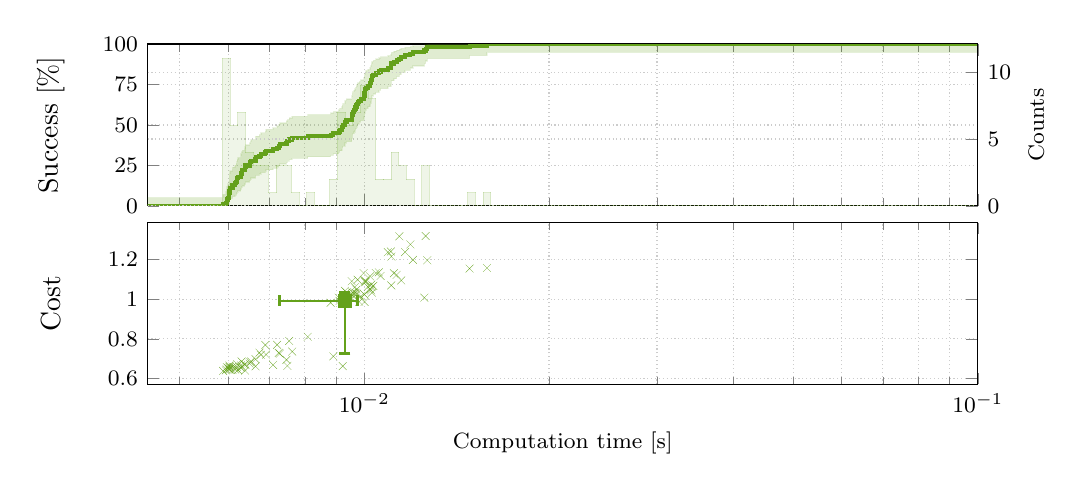
\begin{tikzpicture} [
  xscale=1,
  yscale=1
]
\begin{axis} [
  width=\textwidth,
  height=0.3\textwidth,
  at={(0cm, 0cm)},
  unbounded coords=jump,
  xtick align=inside,
  ytick align=inside,
  axis line style={solid, black},
  name=SuccessAxis,
  xmajorgrids,
  xminorgrids,
  ymajorgrids,
  major grid style={densely dotted, black!20},
  minor grid style={densely dotted, black!20},
  xmin=0.00588612,
  xmax=0.1,
  enlarge x limits=lower,
  ymin=0,
  ymax=100,
  xmode=log,
  xlabel={{\empty}},
  xlabel style={font=\footnotesize},
  xticklabel={{\empty}},
  xticklabel style={font=\footnotesize},
  ylabel={Success [\%]},
  ylabel style={font=\footnotesize, text depth=0.0em, text height=0.5em},
  ylabel absolute,
  ytick={0,25,50,75,100},
 ytick pos={left},
  yticklabel style={font=\footnotesize}
]
\addplot [
  line width=0.5,
  color=pdtgreen,
  mark="none",
  const plot,
  name path={defaultEITstarSuccessUpperConfidence},
  fill opacity=0.2,
  draw opacity=0.1
] table [
  row sep=\\,
  col sep=&
]{
1e-09 & 5.1604\\
0.00588612 & 7.19577\\
0.0059474 & 8.94307\\
0.0059655 & 10.5481\\
0.00597017 & 12.0633\\
0.00599327 & 13.5145\\
0.0060173 & 14.9169\\
0.00602489 & 16.2803\\
0.00602489 & 17.6114\\
0.00602884 & 18.9152\\
0.00603418 & 20.1954\\
0.00603966 & 21.4547\\
0.00609788 & 22.6955\\
0.00609863 & 23.9196\\
0.00615693 & 25.1285\\
0.00618375 & 26.3235\\
0.00619639 & 27.5057\\
0.00620671 & 28.676\\
0.00622265 & 29.8351\\
0.00629034 & 30.9838\\
0.00629521 & 32.1226\\
0.00631089 & 33.2522\\
0.0063266 & 34.3729\\
0.00638327 & 35.4851\\
0.00639226 & 36.5893\\
0.00640424 & 37.6857\\
0.0065039 & 38.7747\\
0.00651843 & 39.8566\\
0.00654104 & 40.9315\\
0.00664883 & 41.9997\\
0.00665069 & 43.0614\\
0.00674792 & 44.1167\\
0.00678266 & 45.1659\\
0.00689982 & 46.2091\\
0.00691614 & 47.2464\\
0.00710231 & 48.2779\\
0.00721006 & 49.3038\\
0.00725425 & 50.3241\\
0.0072835 & 51.339\\
0.00746838 & 52.3485\\
0.00749454 & 53.3527\\
0.00754441 & 54.3517\\
0.00762895 & 55.3454\\
0.0080878 & 56.3341\\
0.00881407 & 57.3177\\
0.00890261 & 58.2962\\
0.00908377 & 59.2697\\
0.00911481 & 60.2382\\
0.00919586 & 61.2017\\
0.00920392 & 62.1603\\
0.00922295 & 63.1139\\
0.00929969 & 64.0625\\
0.00930237 & 65.0062\\
0.00935281 & 65.9449\\
0.00953977 & 66.8786\\
0.00954083 & 67.8073\\
0.00956347 & 68.7309\\
0.00956465 & 69.6495\\
0.00957276 & 70.5629\\
0.00962208 & 71.4712\\
0.00965036 & 72.3742\\
0.00967723 & 73.272\\
0.00970919 & 74.1644\\
0.00972371 & 75.0513\\
0.00975288 & 75.9327\\
0.00981011 & 76.8085\\
0.00986472 & 77.6785\\
0.00997362 & 78.5426\\
0.00999577 & 79.4008\\
0.0100059 & 80.2528\\
0.0100096 & 81.0985\\
0.0100237 & 81.9378\\
0.0100338 & 82.7703\\
0.0100658 & 83.596\\
0.0101347 & 84.4145\\
0.0102214 & 85.2256\\
0.0102293 & 86.0291\\
0.0102607 & 86.8245\\
0.0102672 & 87.6116\\
0.0102807 & 88.3899\\
0.0102917 & 89.1589\\
0.0103445 & 89.9183\\
0.0104391 & 90.6673\\
0.0105609 & 91.4053\\
0.0106312 & 92.1315\\
0.0109231 & 92.8452\\
0.01105 & 93.5451\\
0.011065 & 94.2303\\
0.0110684 & 94.8991\\
0.011176 & 95.5498\\
0.0112911 & 96.1804\\
0.0114044 & 96.7882\\
0.0114834 & 97.3699\\
0.0116527 & 97.921\\
0.0118888 & 98.4357\\
0.0120037 & 98.906\\
0.0125272 & 99.3198\\
0.012589 & 99.6593\\
0.0126652 & 99.896\\
0.0148456 & 99.995\\
0.0158482 & 100\\
0.109124 & 100\\
};

\addplot [
  line width=0.5,
  color=pdtgreen,
  mark="none",
  const plot,
  name path={defaultEITstarSuccessLowerConfidence},
  fill opacity=0.2,
  draw opacity=0.1
] table [
  row sep=\\,
  col sep=&
]{
1e-09 & 0\\
0.00588612 & 0.00501242\\
0.0059474 & 0.103962\\
0.0059655 & 0.340707\\
0.00597017 & 0.680169\\
0.00599327 & 1.09403\\
0.0060173 & 1.56425\\
0.00602489 & 2.07899\\
0.00602489 & 2.63012\\
0.00602884 & 3.21176\\
0.00603418 & 3.81957\\
0.00603966 & 4.45017\\
0.00609788 & 5.10094\\
0.00609863 & 5.76975\\
0.00615693 & 6.45486\\
0.00618375 & 7.15483\\
0.00619639 & 7.86846\\
0.00620671 & 8.59473\\
0.00622265 & 9.33274\\
0.00629034 & 10.0817\\
0.00629521 & 10.8411\\
0.00631089 & 11.6101\\
0.0063266 & 12.3884\\
0.00638327 & 13.1755\\
0.00639226 & 13.9709\\
0.00640424 & 14.7744\\
0.0065039 & 15.5855\\
0.00651843 & 16.404\\
0.00654104 & 17.2297\\
0.00664883 & 18.0622\\
0.00665069 & 18.9015\\
0.00674792 & 19.7472\\
0.00678266 & 20.5992\\
0.00689982 & 21.4574\\
0.00691614 & 22.3215\\
0.00710231 & 23.1915\\
0.00721006 & 24.0673\\
0.00725425 & 24.9487\\
0.0072835 & 25.8356\\
0.00746838 & 26.728\\
0.00749454 & 27.6258\\
0.00754441 & 28.5288\\
0.00762895 & 29.4371\\
0.0080878 & 30.3505\\
0.00881407 & 31.2691\\
0.00890261 & 32.1927\\
0.00908377 & 33.1214\\
0.00911481 & 34.0551\\
0.00919586 & 34.9938\\
0.00920392 & 35.9375\\
0.00922295 & 36.8861\\
0.00929969 & 37.8397\\
0.00930237 & 38.7983\\
0.00935281 & 39.7618\\
0.00953977 & 40.7303\\
0.00954083 & 41.7038\\
0.00956347 & 42.6823\\
0.00956465 & 43.6659\\
0.00957276 & 44.6546\\
0.00962208 & 45.6483\\
0.00965036 & 46.6473\\
0.00967723 & 47.6515\\
0.00970919 & 48.661\\
0.00972371 & 49.6759\\
0.00975288 & 50.6962\\
0.00981011 & 51.7221\\
0.00986472 & 52.7536\\
0.00997362 & 53.7909\\
0.00999577 & 54.8341\\
0.0100059 & 55.8833\\
0.0100096 & 56.9386\\
0.0100237 & 58.0003\\
0.0100338 & 59.0685\\
0.0100658 & 60.1434\\
0.0101347 & 61.2253\\
0.0102214 & 62.3143\\
0.0102293 & 63.4107\\
0.0102607 & 64.5149\\
0.0102672 & 65.6271\\
0.0102807 & 66.7478\\
0.0102917 & 67.8774\\
0.0103445 & 69.0162\\
0.0104391 & 70.1649\\
0.0105609 & 71.324\\
0.0106312 & 72.4943\\
0.0109231 & 73.6765\\
0.01105 & 74.8715\\
0.011065 & 76.0804\\
0.0110684 & 77.3045\\
0.011176 & 78.5453\\
0.0112911 & 79.8046\\
0.0114044 & 81.0848\\
0.0114834 & 82.3886\\
0.0116527 & 83.7197\\
0.0118888 & 85.0831\\
0.0120037 & 86.4855\\
0.0125272 & 87.9367\\
0.012589 & 89.4519\\
0.0126652 & 91.0569\\
0.0148456 & 92.8042\\
0.0158482 & 94.8396\\
0.109124 & 94.8396\\
};

\addplot [
  line width=1,
  color=pdtgreen,
  mark=square*,
  mark size=2,
  const plot,
  fill opacity=0.2,
  draw opacity=0
] fill between [
  of =defaultEITstarSuccessUpperConfidence and defaultEITstarSuccessLowerConfidence
];
\addplot [
  line width=1.5,
  color=pdtgreen,
  mark="none",
  const plot,
  name path={defaultEITstarSuccess}
] table [
  row sep=\\,
  col sep=&
]{
1e-09 & 0\\
0.00588612 & 1\\
0.0059474 & 2\\
0.0059655 & 3\\
0.00597017 & 4\\
0.00599327 & 5\\
0.0060173 & 6\\
0.00602489 & 7\\
0.00602489 & 8\\
0.00602884 & 9\\
0.00603418 & 10\\
0.00603966 & 11\\
0.00609788 & 12\\
0.00609863 & 13\\
0.00615693 & 14\\
0.00618375 & 15\\
0.00619639 & 16\\
0.00620671 & 17\\
0.00622265 & 18\\
0.00629034 & 19\\
0.00629521 & 20\\
0.00631089 & 21\\
0.0063266 & 22\\
0.00638327 & 23\\
0.00639226 & 24\\
0.00640424 & 25\\
0.0065039 & 26\\
0.00651843 & 27\\
0.00654104 & 28\\
0.00664883 & 29\\
0.00665069 & 30\\
0.00674792 & 31\\
0.00678266 & 32\\
0.00689982 & 33\\
0.00691614 & 34\\
0.00710231 & 35\\
0.00721006 & 36\\
0.00725425 & 37\\
0.0072835 & 38\\
0.00746838 & 39\\
0.00749454 & 40\\
0.00754441 & 41\\
0.00762895 & 42\\
0.0080878 & 43\\
0.00881407 & 44\\
0.00890261 & 45\\
0.00908377 & 46\\
0.00911481 & 47\\
0.00919586 & 48\\
0.00920392 & 49\\
0.00922295 & 50\\
0.00929969 & 51\\
0.00930237 & 52\\
0.00935281 & 53\\
0.00953977 & 54\\
0.00954083 & 55\\
0.00956347 & 56\\
0.00956465 & 57\\
0.00957276 & 58\\
0.00962208 & 59\\
0.00965036 & 60\\
0.00967723 & 61\\
0.00970919 & 62\\
0.00972371 & 63\\
0.00975288 & 64\\
0.00981011 & 65\\
0.00986472 & 66\\
0.00997362 & 67\\
0.00999577 & 68\\
0.0100059 & 69\\
0.0100096 & 70\\
0.0100237 & 71\\
0.0100338 & 72\\
0.0100658 & 73\\
0.0101347 & 74\\
0.0102214 & 75\\
0.0102293 & 76\\
0.0102607 & 77\\
0.0102672 & 78\\
0.0102807 & 79\\
0.0102917 & 80\\
0.0103445 & 81\\
0.0104391 & 82\\
0.0105609 & 83\\
0.0106312 & 84\\
0.0109231 & 85\\
0.01105 & 86\\
0.011065 & 87\\
0.0110684 & 88\\
0.011176 & 89\\
0.0112911 & 90\\
0.0114044 & 91\\
0.0114834 & 92\\
0.0116527 & 93\\
0.0118888 & 94\\
0.0120037 & 95\\
0.0125272 & 96\\
0.012589 & 97\\
0.0126652 & 98\\
0.0148456 & 99\\
0.0158482 & 100\\
0.109124 & 100\\
};

\end{axis}

\begin{axis} [
  width=\textwidth,
  height=0.3\textwidth,
  at={(0cm, 0cm)},
  unbounded coords=jump,
  xtick align=inside,
  ytick align=inside,
  axis line style={solid, black},
  name=defaultEITstarISDPA,
  xmajorgrids,
  xminorgrids,
  ymajorgrids,
  major grid style={densely dotted, black!20},
  minor grid style={densely dotted, black!20},
  xmin=0.00588612,
  xmax=0.1,
  enlarge x limits=lower,
  ymin=0,
  ymax=11,
  enlarge y limits=upper,
  xmode=log,
  axis x line=none,
  axis y line*=right,
  xlabel={Computation time [s]},
  xlabel style={font=\footnotesize},
  xtick={{\empty}},
  xticklabel={{\empty}},
  xticklabel style={font=\footnotesize},
  ylabel={Counts},
  ylabel style={font=\footnotesize, text depth=0.0em, text height=0.5em},
  yticklabel style={font=\footnotesize}
]
\addplot [
  line width=0,
  color=pdtgreen,
  mark="none",
  const plot,
  name path={defaultEITstarInitialSolutionDurationHistogram},
  fill=pdtgreen,
  fill opacity=0.1,
  draw opacity=0.2
] table [
  row sep=\\,
  col sep=&
]{
0.00570601 & 0\\
0.00570601 & 0\\
0.00587252 & 11\\
0.0060439 & 6\\
0.00622027 & 7\\
0.00640179 & 4\\
0.00658861 & 3\\
0.00678089 & 3\\
0.00697877 & 1\\
0.00718243 & 3\\
0.00739203 & 3\\
0.00760774 & 1\\
0.00782975 & 0\\
0.00805825 & 1\\
0.0082934 & 0\\
0.00853543 & 0\\
0.00878451 & 2\\
0.00904086 & 7\\
0.0093047 & 6\\
0.00957623 & 7\\
0.00985569 & 9\\
0.0101433 & 8\\
0.0104393 & 2\\
0.0107439 & 2\\
0.0110575 & 4\\
0.0113802 & 3\\
0.0117123 & 2\\
0.0120541 & 0\\
0.0124058 & 3\\
0.0127679 & 0\\
0.0131405 & 0\\
0.0135239 & 0\\
0.0139186 & 0\\
0.0143248 & 0\\
0.0147428 & 1\\
0.015173 & 0\\
0.0156158 & 1\\
0.0160715 & 0\\
0.0165405 & 0\\
0.0170232 & 0\\
0.01752 & 0\\
0.0180313 & 0\\
0.0185575 & 0\\
0.019099 & 0\\
0.0196564 & 0\\
0.02023 & 0\\
0.0208203 & 0\\
0.0214279 & 0\\
0.0220532 & 0\\
0.0226968 & 0\\
0.0233592 & 0\\
0.0240408 & 0\\
0.0247424 & 0\\
0.0254644 & 0\\
0.0262076 & 0\\
0.0269724 & 0\\
0.0277595 & 0\\
0.0285696 & 0\\
0.0294033 & 0\\
0.0302613 & 0\\
0.0311444 & 0\\
0.0320533 & 0\\
0.0329887 & 0\\
0.0339514 & 0\\
0.0349422 & 0\\
0.0359619 & 0\\
0.0370113 & 0\\
0.0380914 & 0\\
0.039203 & 0\\
0.040347 & 0\\
0.0415245 & 0\\
0.0427362 & 0\\
0.0439834 & 0\\
0.0452669 & 0\\
0.0465879 & 0\\
0.0479475 & 0\\
0.0493467 & 0\\
0.0507867 & 0\\
0.0522688 & 0\\
0.0537941 & 0\\
0.055364 & 0\\
0.0569796 & 0\\
0.0586424 & 0\\
0.0603538 & 0\\
0.062115 & 0\\
0.0639277 & 0\\
0.0657933 & 0\\
0.0677133 & 0\\
0.0696893 & 0\\
0.071723 & 0\\
0.073816 & 0\\
0.0759702 & 0\\
0.0781872 & 0\\
0.0804688 & 0\\
0.0828171 & 0\\
0.0852339 & 0\\
0.0877213 & 0\\
0.0902812 & 0\\
0.0929158 & 0\\
0.0956273 & 0\\
0.0984179 & 0\\
0.0984179 & 0\\
};

\end{axis}

\begin{axis} [
  width=\textwidth,
  height=0.3\textwidth,
  at={($(SuccessAxis.south) - (0.0em, 0.6em)$)},
  unbounded coords=jump,
  xtick align=inside,
  ytick align=inside,
  axis line style={solid, black},
  name=defaultEITstarInitialSolutionScatterAxis,
  anchor=north,
  xmajorgrids,
  xminorgrids,
  ymajorgrids,
  major grid style={densely dotted, black!20},
  minor grid style={densely dotted, black!20},
  xmin=0.00588612,
  xmax=0.1,
  enlarge x limits=lower,
  xmode=log,
  xlabel={Computation time [s]},
  xlabel style={font=\footnotesize},
  xticklabel style={font=\footnotesize},
  ylabel={Cost},
  ylabel style={font=\footnotesize, text depth=0.0em, text height=0.5em},
  ylabel absolute,
  yticklabel style={font=\footnotesize}
]
\addplot [
  line width=0.1,
  color=pdtgreen,
  mark=x,
  mark size=2,
  only marks,
  name path={defaultEITstarInitialSolutionScatterPlotlineWidth}
] table [
  row sep=\\,
  col sep=&
]{
0.0148456 & 1.15486\\
0.0102917 & 1.03327\\
0.0102807 & 1.06121\\
0.0110684 & 1.21487\\
0.0100338 & 1.0863\\
0.00602884 & 0.666451\\
0.0103445 & 1.06746\\
0.0100059 & 1.02434\\
0.00638327 & 0.672229\\
0.00956465 & 1.03412\\
0.01105 & 1.24092\\
0.00615693 & 0.646137\\
0.0158482 & 1.15763\\
0.00953977 & 1.00487\\
0.0102293 & 1.05023\\
0.00975288 & 1.09836\\
0.00588612 & 0.638522\\
0.00639226 & 0.640464\\
0.00986472 & 1.01491\\
0.00922295 & 0.662616\\
0.00640424 & 0.668481\\
0.0100096 & 0.986398\\
0.00609863 & 0.643166\\
0.00664883 & 0.662026\\
0.00911481 & 0.991683\\
0.0080878 & 0.810879\\
0.00619639 & 0.659516\\
0.0114044 & 1.31763\\
0.00629034 & 0.655348\\
0.00602489 & 0.649312\\
0.0060173 & 0.646705\\
0.00678266 & 0.719902\\
0.00746838 & 0.694221\\
0.00929969 & 1.04277\\
0.00654104 & 0.686061\\
0.0063266 & 0.659409\\
0.0116527 & 1.2378\\
0.0100658 & 1.09016\\
0.00919586 & 0.990447\\
0.00691614 & 0.72117\\
0.00651843 & 0.68217\\
0.0101347 & 1.06307\\
0.00890261 & 0.7124\\
0.00972371 & 1.02715\\
0.0102672 & 1.0739\\
0.0102214 & 1.11562\\
0.0105609 & 1.13588\\
0.011065 & 1.06969\\
0.00629521 & 0.666117\\
0.00603418 & 0.660681\\
0.00762895 & 0.736191\\
0.00602489 & 0.656026\\
0.011176 & 1.13105\\
0.00631089 & 0.686433\\
0.0109231 & 1.237\\
0.00674792 & 0.730591\\
0.0114834 & 1.09491\\
0.0126652 & 1.19668\\
0.00599327 & 0.65424\\
0.0100237 & 1.09336\\
0.00609788 & 0.659951\\
0.00954083 & 1.09098\\
0.00908377 & 1.00808\\
0.00710231 & 0.668986\\
0.00665069 & 0.697843\\
0.00754441 & 0.789642\\
0.00881407 & 0.982366\\
0.0059655 & 0.646511\\
0.0104391 & 1.13224\\
0.00620671 & 0.672339\\
0.00981011 & 0.987497\\
0.00725425 & 0.729736\\
0.012589 & 1.3188\\
0.0112911 & 1.12308\\
0.00622265 & 0.643075\\
0.00597017 & 0.658148\\
0.00689982 & 0.769375\\
0.00749454 & 0.664167\\
0.0125272 & 1.00818\\
0.00997362 & 1.1318\\
0.0106312 & 1.11761\\
0.0059474 & 0.641948\\
0.0102607 & 1.04492\\
0.0118888 & 1.27679\\
0.0072835 & 0.725844\\
0.00930237 & 0.978179\\
0.00962208 & 1.03418\\
0.00920392 & 1.00377\\
0.00999577 & 1.02422\\
0.00935281 & 1.03464\\
0.00603966 & 0.64548\\
0.00956347 & 1.01835\\
0.00618375 & 0.651936\\
0.00957276 & 1.0222\\
0.00967723 & 1.03267\\
0.00970919 & 1.04845\\
0.00965036 & 1.06067\\
0.00721006 & 0.770434\\
0.0120037 & 1.19852\\
0.0065039 & 0.675421\\
};

\addplot [
  line width=1,
  color=pdtgreen,
  mark=square*,
  mark size=2,
  only marks,
  const plot,
  name path={defaultEITstarMedianInitialSolution}
] table [
  row sep=\\,
  col sep=&
]{
0.00929969 & 0.991683\\
};

\addplot [
  line width=1,
  color=pdtgreen,
  mark=|,
  mark size=2,
  const plot,
  name path={defaultEITstarMedianInitialSolutionDurationConfidenceInterval}
] table [
  row sep=\\,
  col sep=&
]{
0.0072835 & 0.991683\\
0.00975288 & 0.991683\\
};

\addplot [
  line width=1,
  color=pdtgreen,
  mark=-,
  mark size=2,
  const plot,
  name path={defaultEITstarMedianInitialSolutionDurationConfidenceInterval}
] table [
  row sep=\\,
  col sep=&
]{
0.00929969 & 0.725844\\
0.00929969 & 1.03412\\
};

\end{axis}

\end{tikzpicture}%
\captionof{figure}{\footnotesize \textbf{Top:} Histogram and associated empirical distribution function (EDF) of EIT* with a Clopper-Pearson (nonparametric) 99\% confidence interval for the underlying CDF. \textbf{Bottom:} All initial solutions of EIT* and their median with a nonparametric 99\% confidence interval.}
\end{center}
\subsection{Cost Evolution}\label{sec:defaultEITstar-cost-evolution}
\begin{center}
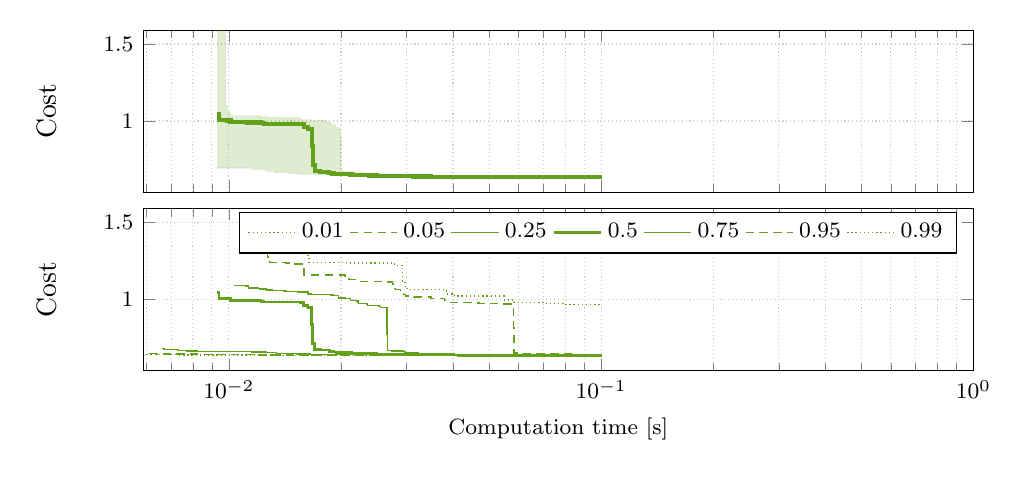
\begin{tikzpicture} [
  xscale=1,
  yscale=1
]
\begin{axis} [
  width=\textwidth,
  height=0.3\textwidth,
  at={(0cm, 0cm)},
  unbounded coords=jump,
  xtick align=inside,
  ytick align=inside,
  axis line style={solid, black},
  name=defaultEITstarMedianCostAxis,
  xmajorgrids,
  xminorgrids,
  ymajorgrids,
  major grid style={densely dotted, black!20},
  minor grid style={densely dotted, black!20},
  xmin=0.00588612,
  xmax=1,
  ymax=1.58998,
  xmode=log,
  xlabel={{\empty}},
  xlabel style={font=\footnotesize},
  xticklabel={{\empty}},
  xticklabel style={font=\footnotesize},
  ylabel={Cost},
  ylabel style={font=\footnotesize, text depth=0.0em, text height=0.5em},
  ylabel absolute,
  yticklabel style={font=\footnotesize}
]
\addplot [
  line width=0.5,
  color=pdtgreen,
  mark="none",
  const plot,
  name path={defaultEITstarMedianCostEvolutionUpperConfidence},
  fill opacity=0.2,
  draw opacity=0.1
] table [
  row sep=\\,
  col sep=&
]{
0.0093 & 4.76994\\
0.0097 & 4.76994\\
0.0098 & 1.09836\\
0.0099 & 1.06067\\
0.01 & 1.04845\\
0.0101 & 1.03464\\
0.0102 & 1.03464\\
0.0103 & 1.03418\\
0.0115 & 1.03418\\
0.0116 & 1.03412\\
0.0117 & 1.03327\\
0.012 & 1.03327\\
0.0121 & 1.0323\\
0.0122 & 1.02714\\
0.0125 & 1.02714\\
0.0126 & 1.02643\\
0.0127 & 1.02422\\
0.0132 & 1.02422\\
0.0133 & 1.0222\\
0.0142 & 1.0222\\
0.0143 & 1.02207\\
0.0153 & 1.02207\\
0.0154 & 1.01835\\
0.0155 & 1.01835\\
0.0156 & 1.00931\\
0.0157 & 1.00914\\
0.0158 & 1.009\\
0.0162 & 1.009\\
0.0163 & 1.00818\\
0.0166 & 1.00818\\
0.0167 & 1.00332\\
0.0168 & 1.00282\\
0.0182 & 1.00282\\
0.0183 & 0.994615\\
0.0184 & 0.994615\\
0.0185 & 0.99226\\
0.0186 & 0.991677\\
0.0187 & 0.989433\\
0.0188 & 0.983085\\
0.0189 & 0.978186\\
0.019 & 0.978186\\
0.0191 & 0.974267\\
0.0192 & 0.974267\\
0.0193 & 0.958478\\
0.0197 & 0.958478\\
0.0198 & 0.947187\\
0.0199 & 0.906421\\
0.02 & 0.678117\\
0.0202 & 0.678117\\
0.0203 & 0.671028\\
0.0219 & 0.671028\\
0.022 & 0.665696\\
0.0229 & 0.665696\\
0.023 & 0.664217\\
0.0231 & 0.66015\\
0.0232 & 0.66015\\
0.0233 & 0.658994\\
0.0245 & 0.658994\\
0.0246 & 0.657223\\
0.025 & 0.657223\\
0.0251 & 0.655746\\
0.0255 & 0.655746\\
0.0256 & 0.652923\\
0.0257 & 0.652546\\
0.0258 & 0.651399\\
0.0259 & 0.651193\\
0.0261 & 0.651193\\
0.0262 & 0.649619\\
0.0263 & 0.648806\\
0.0266 & 0.648806\\
0.0267 & 0.647961\\
0.0274 & 0.647961\\
0.0275 & 0.647753\\
0.0281 & 0.647753\\
0.0282 & 0.646055\\
0.0291 & 0.646055\\
0.0292 & 0.645453\\
0.0296 & 0.645453\\
0.0297 & 0.645349\\
0.03 & 0.645349\\
0.0301 & 0.645279\\
0.0307 & 0.645279\\
0.0308 & 0.645271\\
0.0311 & 0.645271\\
0.0312 & 0.644368\\
0.0317 & 0.644368\\
0.0318 & 0.644238\\
0.0319 & 0.644238\\
0.032 & 0.643994\\
0.0321 & 0.643743\\
0.033 & 0.643743\\
0.0331 & 0.643673\\
0.0332 & 0.643582\\
0.0348 & 0.643582\\
0.0349 & 0.643576\\
0.0358 & 0.643576\\
0.0359 & 0.642633\\
0.036 & 0.642501\\
0.0363 & 0.642501\\
0.0364 & 0.6407\\
0.0367 & 0.6407\\
0.0368 & 0.640443\\
0.0373 & 0.640443\\
0.0374 & 0.640425\\
0.0376 & 0.640425\\
0.0377 & 0.640161\\
0.0378 & 0.640161\\
0.0379 & 0.63994\\
0.0387 & 0.63994\\
0.0388 & 0.639845\\
0.039 & 0.639845\\
0.0391 & 0.639518\\
0.0396 & 0.639518\\
0.0397 & 0.639187\\
0.0403 & 0.639187\\
0.0404 & 0.638935\\
0.0405 & 0.638935\\
0.0406 & 0.638857\\
0.0415 & 0.638857\\
0.0416 & 0.638717\\
0.0441 & 0.638717\\
0.0442 & 0.638715\\
0.0443 & 0.638715\\
0.0444 & 0.638559\\
0.0446 & 0.638559\\
0.0447 & 0.638538\\
0.0459 & 0.638538\\
0.046 & 0.638536\\
0.0464 & 0.638536\\
0.0465 & 0.638459\\
0.0467 & 0.638459\\
0.0468 & 0.638447\\
0.0473 & 0.638447\\
0.0474 & 0.638258\\
0.048 & 0.638258\\
0.0481 & 0.638156\\
0.0482 & 0.63801\\
0.0485 & 0.63801\\
0.0486 & 0.637931\\
0.0488 & 0.637931\\
0.0489 & 0.637909\\
0.049 & 0.637894\\
0.0491 & 0.637795\\
0.0492 & 0.63773\\
0.0496 & 0.63773\\
0.0497 & 0.637702\\
0.0498 & 0.63762\\
0.05 & 0.63762\\
0.0501 & 0.637533\\
0.0506 & 0.637533\\
0.0507 & 0.637264\\
0.0528 & 0.637264\\
0.0529 & 0.637161\\
0.0539 & 0.637161\\
0.054 & 0.63714\\
0.0541 & 0.63705\\
0.0554 & 0.63705\\
0.0555 & 0.636908\\
0.0556 & 0.636908\\
0.0557 & 0.636863\\
0.0573 & 0.636863\\
0.0574 & 0.636845\\
0.0578 & 0.636845\\
0.0579 & 0.636704\\
0.0595 & 0.636704\\
0.0596 & 0.636697\\
0.0597 & 0.636638\\
0.0624 & 0.636638\\
0.0625 & 0.636625\\
0.0629 & 0.636625\\
0.063 & 0.636617\\
0.0631 & 0.636592\\
0.0633 & 0.636592\\
0.0634 & 0.636405\\
0.064 & 0.636405\\
0.0641 & 0.636352\\
0.0652 & 0.636352\\
0.0653 & 0.636344\\
0.0674 & 0.636344\\
0.0675 & 0.636243\\
0.0676 & 0.636181\\
0.0707 & 0.636181\\
0.0708 & 0.636136\\
0.0727 & 0.636136\\
0.0728 & 0.635966\\
0.0729 & 0.635937\\
0.0752 & 0.635937\\
0.0753 & 0.63591\\
0.0759 & 0.63591\\
0.076 & 0.63587\\
0.0761 & 0.63568\\
0.0765 & 0.63568\\
0.0766 & 0.635661\\
0.0777 & 0.635661\\
0.0778 & 0.635482\\
0.0792 & 0.635482\\
0.0793 & 0.635408\\
0.0813 & 0.635408\\
0.0814 & 0.635406\\
0.0834 & 0.635406\\
0.0835 & 0.635313\\
0.085 & 0.635313\\
0.0851 & 0.635295\\
0.0884 & 0.635295\\
0.0885 & 0.635261\\
0.0899 & 0.635261\\
0.09 & 0.635241\\
0.0901 & 0.635225\\
0.0942 & 0.635225\\
0.0943 & 0.635172\\
0.0957 & 0.635172\\
0.0958 & 0.635129\\
0.0984 & 0.635129\\
0.0985 & 0.635088\\
0.0999 & 0.635088\\
0.1 & 0.635088\\
};

\addplot [
  line width=0.5,
  color=pdtgreen,
  mark="none",
  const plot,
  name path={defaultEITstarMedianCostEvolutionLowerConfidence},
  fill opacity=0.2,
  draw opacity=0.1
] table [
  row sep=\\,
  col sep=&
]{
0.0093 & 0.694221\\
0.01 & 0.694221\\
0.0101 & 0.693739\\
0.0113 & 0.693739\\
0.0114 & 0.692855\\
0.0115 & 0.686433\\
0.0116 & 0.686433\\
0.0117 & 0.685642\\
0.0124 & 0.685642\\
0.0125 & 0.681338\\
0.0126 & 0.673654\\
0.0131 & 0.673654\\
0.0132 & 0.668986\\
0.0133 & 0.6645\\
0.0142 & 0.6645\\
0.0143 & 0.664167\\
0.0145 & 0.664167\\
0.0146 & 0.661055\\
0.0148 & 0.661055\\
0.0149 & 0.658784\\
0.015 & 0.658407\\
0.0151 & 0.658407\\
0.0152 & 0.657468\\
0.0155 & 0.657468\\
0.0156 & 0.656745\\
0.0157 & 0.656314\\
0.0158 & 0.656314\\
0.0159 & 0.656026\\
0.0163 & 0.656026\\
0.0164 & 0.653611\\
0.0165 & 0.651679\\
0.0175 & 0.651679\\
0.0176 & 0.6511\\
0.0186 & 0.6511\\
0.0187 & 0.649312\\
0.0188 & 0.649312\\
0.0189 & 0.648922\\
0.019 & 0.648922\\
0.0191 & 0.648225\\
0.0192 & 0.648225\\
0.0193 & 0.64819\\
0.0203 & 0.64819\\
0.0204 & 0.647961\\
0.0209 & 0.647961\\
0.021 & 0.647849\\
0.0211 & 0.64598\\
0.0213 & 0.64598\\
0.0214 & 0.645685\\
0.0215 & 0.644984\\
0.0221 & 0.644984\\
0.0222 & 0.644653\\
0.0224 & 0.644653\\
0.0225 & 0.644638\\
0.0226 & 0.644262\\
0.023 & 0.644262\\
0.0231 & 0.643204\\
0.0232 & 0.643041\\
0.0233 & 0.64287\\
0.0234 & 0.642799\\
0.0235 & 0.642501\\
0.0242 & 0.642501\\
0.0243 & 0.642179\\
0.0244 & 0.641933\\
0.0245 & 0.641663\\
0.0246 & 0.641663\\
0.0247 & 0.641267\\
0.0249 & 0.641267\\
0.025 & 0.641232\\
0.0251 & 0.641232\\
0.0252 & 0.641187\\
0.0253 & 0.641187\\
0.0254 & 0.641127\\
0.0257 & 0.641127\\
0.0258 & 0.640773\\
0.026 & 0.640773\\
0.0261 & 0.640609\\
0.0262 & 0.640164\\
0.0266 & 0.640164\\
0.0267 & 0.640006\\
0.0274 & 0.640006\\
0.0275 & 0.639888\\
0.0276 & 0.639845\\
0.0277 & 0.639767\\
0.0279 & 0.639767\\
0.028 & 0.639723\\
0.0281 & 0.639651\\
0.0282 & 0.639625\\
0.03 & 0.639625\\
0.0301 & 0.639499\\
0.0303 & 0.639499\\
0.0304 & 0.639333\\
0.0305 & 0.639333\\
0.0306 & 0.639271\\
0.0307 & 0.639035\\
0.0308 & 0.638935\\
0.0309 & 0.638935\\
0.031 & 0.638557\\
0.0311 & 0.638436\\
0.0312 & 0.638436\\
0.0313 & 0.638378\\
0.0326 & 0.638378\\
0.0327 & 0.638301\\
0.0333 & 0.638301\\
0.0334 & 0.638258\\
0.0335 & 0.63822\\
0.0337 & 0.63822\\
0.0338 & 0.63814\\
0.0339 & 0.63814\\
0.034 & 0.638025\\
0.0343 & 0.638025\\
0.0344 & 0.637931\\
0.0345 & 0.637817\\
0.0346 & 0.637739\\
0.0347 & 0.63773\\
0.0348 & 0.63773\\
0.0349 & 0.637711\\
0.0352 & 0.637711\\
0.0353 & 0.637698\\
0.0354 & 0.63764\\
0.0363 & 0.63764\\
0.0364 & 0.637586\\
0.0366 & 0.637586\\
0.0367 & 0.637533\\
0.0368 & 0.63726\\
0.0369 & 0.63726\\
0.037 & 0.637242\\
0.0373 & 0.637242\\
0.0374 & 0.637161\\
0.0376 & 0.637161\\
0.0377 & 0.63705\\
0.0384 & 0.63705\\
0.0385 & 0.636962\\
0.0391 & 0.636962\\
0.0392 & 0.636957\\
0.0394 & 0.636957\\
0.0395 & 0.636888\\
0.0396 & 0.636817\\
0.0397 & 0.636817\\
0.0398 & 0.636795\\
0.0399 & 0.63678\\
0.0402 & 0.63678\\
0.0403 & 0.636702\\
0.0406 & 0.636702\\
0.0407 & 0.636697\\
0.0418 & 0.636697\\
0.0419 & 0.636625\\
0.042 & 0.636625\\
0.0421 & 0.636539\\
0.0435 & 0.636539\\
0.0436 & 0.636538\\
0.0446 & 0.636538\\
0.0447 & 0.636284\\
0.0448 & 0.636284\\
0.0449 & 0.636277\\
0.0451 & 0.636277\\
0.0452 & 0.636188\\
0.0458 & 0.636188\\
0.0459 & 0.636048\\
0.0464 & 0.636048\\
0.0465 & 0.635905\\
0.0467 & 0.635905\\
0.0468 & 0.635844\\
0.0469 & 0.635831\\
0.0471 & 0.635831\\
0.0472 & 0.635829\\
0.0482 & 0.635829\\
0.0483 & 0.635826\\
0.0494 & 0.635826\\
0.0495 & 0.635816\\
0.05 & 0.635816\\
0.0501 & 0.635811\\
0.0522 & 0.635811\\
0.0523 & 0.635708\\
0.0524 & 0.6357\\
0.0527 & 0.6357\\
0.0528 & 0.635687\\
0.053 & 0.635687\\
0.0531 & 0.635687\\
0.0533 & 0.635687\\
0.0534 & 0.635681\\
0.0535 & 0.63568\\
0.0537 & 0.63568\\
0.0538 & 0.635631\\
0.054 & 0.635631\\
0.0541 & 0.635599\\
0.0544 & 0.635599\\
0.0545 & 0.635547\\
0.0566 & 0.635547\\
0.0567 & 0.63548\\
0.0569 & 0.63548\\
0.057 & 0.635449\\
0.0574 & 0.635449\\
0.0575 & 0.63544\\
0.0579 & 0.63544\\
0.058 & 0.635406\\
0.0584 & 0.635406\\
0.0585 & 0.63538\\
0.0594 & 0.63538\\
0.0595 & 0.635332\\
0.0602 & 0.635332\\
0.0603 & 0.635291\\
0.061 & 0.635291\\
0.0611 & 0.635235\\
0.0615 & 0.635235\\
0.0616 & 0.6352\\
0.063 & 0.6352\\
0.0631 & 0.635176\\
0.0632 & 0.635163\\
0.0637 & 0.635163\\
0.0638 & 0.635129\\
0.0668 & 0.635129\\
0.0669 & 0.635091\\
0.067 & 0.635072\\
0.0694 & 0.635072\\
0.0695 & 0.635044\\
0.0696 & 0.635014\\
0.0697 & 0.63501\\
0.0705 & 0.63501\\
0.0706 & 0.634939\\
0.0711 & 0.634939\\
0.0712 & 0.634875\\
0.0713 & 0.634866\\
0.0752 & 0.634866\\
0.0753 & 0.634796\\
0.0754 & 0.634737\\
0.0766 & 0.634737\\
0.0767 & 0.634652\\
0.0792 & 0.634652\\
0.0793 & 0.634558\\
0.0794 & 0.634557\\
0.0835 & 0.634557\\
0.0836 & 0.634487\\
0.0841 & 0.634487\\
0.0842 & 0.634471\\
0.0843 & 0.634453\\
0.085 & 0.634453\\
0.0851 & 0.634445\\
0.0884 & 0.634445\\
0.0885 & 0.634408\\
0.0892 & 0.634408\\
0.0893 & 0.634401\\
0.0916 & 0.634401\\
0.0917 & 0.634376\\
0.0929 & 0.634376\\
0.093 & 0.634373\\
0.0945 & 0.634373\\
0.0946 & 0.634313\\
0.0984 & 0.634313\\
0.0985 & 0.634254\\
0.0986 & 0.634234\\
0.0999 & 0.634234\\
0.1 & 0.634234\\
};

\addplot [
  line width=1,
  color=pdtgreen,
  mark=square*,
  mark size=2,
  const plot,
  fill opacity=0.2,
  draw opacity=0
] fill between [
  of =defaultEITstarMedianCostEvolutionUpperConfidence and defaultEITstarMedianCostEvolutionLowerConfidence
];
\addplot [
  line width=1.5,
  color=pdtgreen,
  mark="none",
  const plot,
  name path={defaultEITstarMedianCostEvolution}
] table [
  row sep=\\,
  col sep=&
]{
0.0001 & inf\\
0.0092 & inf\\
0.0093 & 1.04277\\
0.0094 & 1.00808\\
0.0095 & 1.00808\\
0.0096 & 1.00487\\
0.0098 & 1.00487\\
0.0099 & 1.00377\\
0.01 & 1.00377\\
0.0101 & 0.991683\\
0.0111 & 0.991683\\
0.0112 & 0.990447\\
0.0121 & 0.990447\\
0.0122 & 0.986398\\
0.0123 & 0.985568\\
0.0124 & 0.983085\\
0.0127 & 0.983085\\
0.0128 & 0.982366\\
0.0155 & 0.982366\\
0.0156 & 0.978179\\
0.0158 & 0.978179\\
0.0159 & 0.958478\\
0.0162 & 0.958478\\
0.0163 & 0.949753\\
0.0164 & 0.947487\\
0.0166 & 0.947487\\
0.0167 & 0.836544\\
0.0168 & 0.7124\\
0.0169 & 0.7124\\
0.017 & 0.673187\\
0.0175 & 0.673187\\
0.0176 & 0.671028\\
0.0185 & 0.671028\\
0.0186 & 0.661055\\
0.0187 & 0.660125\\
0.0188 & 0.660125\\
0.0189 & 0.658933\\
0.019 & 0.658933\\
0.0191 & 0.657468\\
0.0192 & 0.657468\\
0.0193 & 0.657192\\
0.0194 & 0.657192\\
0.0195 & 0.656863\\
0.0196 & 0.656745\\
0.0197 & 0.656655\\
0.0201 & 0.656655\\
0.0202 & 0.656421\\
0.0203 & 0.656394\\
0.0207 & 0.656394\\
0.0208 & 0.656314\\
0.0209 & 0.656314\\
0.021 & 0.655263\\
0.0211 & 0.6534\\
0.0212 & 0.652423\\
0.0213 & 0.652423\\
0.0214 & 0.651815\\
0.0219 & 0.651815\\
0.022 & 0.651399\\
0.0224 & 0.651399\\
0.0225 & 0.650046\\
0.0229 & 0.650046\\
0.023 & 0.649312\\
0.0231 & 0.648922\\
0.0232 & 0.647961\\
0.0233 & 0.647945\\
0.0235 & 0.647945\\
0.0236 & 0.647849\\
0.0237 & 0.647128\\
0.0238 & 0.646055\\
0.0248 & 0.646055\\
0.0249 & 0.646001\\
0.025 & 0.645004\\
0.0252 & 0.645004\\
0.0253 & 0.644984\\
0.0257 & 0.644984\\
0.0258 & 0.644638\\
0.0259 & 0.644546\\
0.026 & 0.644268\\
0.0261 & 0.644268\\
0.0262 & 0.644201\\
0.0266 & 0.644201\\
0.0267 & 0.643284\\
0.0274 & 0.643284\\
0.0275 & 0.642714\\
0.0276 & 0.641941\\
0.0277 & 0.641696\\
0.0282 & 0.641696\\
0.0283 & 0.641663\\
0.0292 & 0.641663\\
0.0293 & 0.641587\\
0.0295 & 0.641587\\
0.0296 & 0.641267\\
0.0302 & 0.641267\\
0.0303 & 0.641009\\
0.0304 & 0.641009\\
0.0305 & 0.64088\\
0.0306 & 0.640823\\
0.0308 & 0.640823\\
0.0309 & 0.640609\\
0.0312 & 0.640609\\
0.0313 & 0.640073\\
0.032 & 0.640073\\
0.0321 & 0.639982\\
0.0322 & 0.63976\\
0.0337 & 0.63976\\
0.0338 & 0.639753\\
0.0343 & 0.639753\\
0.0344 & 0.639651\\
0.0347 & 0.639651\\
0.0348 & 0.639187\\
0.035 & 0.639187\\
0.0351 & 0.639069\\
0.0359 & 0.639069\\
0.036 & 0.638981\\
0.0361 & 0.638981\\
0.0362 & 0.638935\\
0.0363 & 0.638935\\
0.0364 & 0.638857\\
0.0367 & 0.638857\\
0.0368 & 0.63854\\
0.0369 & 0.638469\\
0.0372 & 0.638469\\
0.0373 & 0.638436\\
0.0374 & 0.638258\\
0.0383 & 0.638258\\
0.0384 & 0.637931\\
0.0391 & 0.637931\\
0.0392 & 0.637854\\
0.0396 & 0.637854\\
0.0397 & 0.63773\\
0.0398 & 0.63764\\
0.0402 & 0.63764\\
0.0403 & 0.63762\\
0.0404 & 0.63762\\
0.0405 & 0.637586\\
0.0412 & 0.637586\\
0.0413 & 0.637453\\
0.0414 & 0.637242\\
0.0442 & 0.637242\\
0.0443 & 0.637159\\
0.0444 & 0.63705\\
0.0463 & 0.63705\\
0.0464 & 0.636863\\
0.0477 & 0.636863\\
0.0478 & 0.636841\\
0.0479 & 0.636795\\
0.048 & 0.636795\\
0.0481 & 0.636702\\
0.0482 & 0.636697\\
0.0497 & 0.636697\\
0.0498 & 0.636613\\
0.05 & 0.636613\\
0.0501 & 0.636577\\
0.0505 & 0.636577\\
0.0506 & 0.636569\\
0.0517 & 0.636569\\
0.0518 & 0.636539\\
0.0526 & 0.636539\\
0.0527 & 0.636486\\
0.0539 & 0.636486\\
0.054 & 0.636286\\
0.0542 & 0.636286\\
0.0543 & 0.63624\\
0.0557 & 0.63624\\
0.0558 & 0.63622\\
0.0567 & 0.63622\\
0.0568 & 0.636188\\
0.0569 & 0.636136\\
0.057 & 0.636045\\
0.0571 & 0.636012\\
0.0584 & 0.636012\\
0.0585 & 0.63601\\
0.0589 & 0.63601\\
0.059 & 0.635831\\
0.0594 & 0.635831\\
0.0595 & 0.635814\\
0.0596 & 0.635687\\
0.0597 & 0.635687\\
0.0598 & 0.635639\\
0.0602 & 0.635639\\
0.0603 & 0.635631\\
0.0612 & 0.635631\\
0.0613 & 0.6356\\
0.0614 & 0.6356\\
0.0615 & 0.635599\\
0.063 & 0.635599\\
0.0631 & 0.635581\\
0.0632 & 0.635545\\
0.0635 & 0.635545\\
0.0636 & 0.635495\\
0.0637 & 0.635482\\
0.066 & 0.635482\\
0.0661 & 0.63548\\
0.0664 & 0.63548\\
0.0665 & 0.635406\\
0.0668 & 0.635406\\
0.0669 & 0.635403\\
0.0676 & 0.635403\\
0.0677 & 0.635385\\
0.0678 & 0.63537\\
0.0695 & 0.63537\\
0.0696 & 0.635366\\
0.0708 & 0.635366\\
0.0709 & 0.635313\\
0.0718 & 0.635313\\
0.0719 & 0.635261\\
0.0728 & 0.635261\\
0.0729 & 0.635225\\
0.0747 & 0.635225\\
0.0748 & 0.6352\\
0.0752 & 0.6352\\
0.0753 & 0.635173\\
0.0766 & 0.635173\\
0.0767 & 0.635172\\
0.0769 & 0.635172\\
0.077 & 0.635129\\
0.0776 & 0.635129\\
0.0777 & 0.635112\\
0.0778 & 0.635112\\
0.0779 & 0.635104\\
0.0794 & 0.635104\\
0.0795 & 0.635088\\
0.0798 & 0.635088\\
0.0799 & 0.635086\\
0.0814 & 0.635086\\
0.0815 & 0.635081\\
0.0834 & 0.635081\\
0.0835 & 0.635076\\
0.0841 & 0.635076\\
0.0842 & 0.635044\\
0.085 & 0.635044\\
0.0851 & 0.634912\\
0.0884 & 0.634912\\
0.0885 & 0.634866\\
0.091 & 0.634866\\
0.0911 & 0.634859\\
0.0925 & 0.634859\\
0.0926 & 0.634818\\
0.0942 & 0.634818\\
0.0943 & 0.634785\\
0.097 & 0.634785\\
0.0971 & 0.634679\\
0.0985 & 0.634679\\
0.0986 & 0.634652\\
0.0999 & 0.634652\\
0.1 & 0.634652\\
};

\end{axis}

\begin{axis} [
  width=\textwidth,
  height=0.3\textwidth,
  at={($(defaultEITstarMedianCostAxis.south) - (0.0em, 0.6em)$)},
  unbounded coords=jump,
  xtick align=inside,
  ytick align=inside,
  axis line style={solid, black},
  name=defaultEITstarCostPercentileEvolutionAxis,
  anchor=north,
  xmajorgrids,
  xminorgrids,
  ymajorgrids,
  major grid style={densely dotted, black!20},
  minor grid style={densely dotted, black!20},
  xmin=0.00588612,
  xmax=1,
  ymax=1.58998,
  xmode=log,
  xlabel={Computation time [s]},
  xlabel style={font=\footnotesize},
  xticklabel style={font=\footnotesize},
  ylabel={Cost},
  ylabel style={font=\footnotesize, text depth=0.0em, text height=0.5em},
  ylabel absolute,
  yticklabel style={font=\footnotesize},
  legend style={font=\footnotesize, legend cell align=left, legend columns=-1}
]
\addplot [
  line width=0.5,
  color=pdtgreen,
  mark="none",
  const plot,
  densely dotted,
  name path={defaultEITstarpercentile0.01CostEvolution}
] table [
  row sep=\\,
  col sep=&
]{
0.0001 & inf\\
0.0059 & inf\\
0.006 & 0.641948\\
0.0063 & 0.641948\\
0.0064 & 0.640464\\
0.0071 & 0.640464\\
0.0072 & 0.640399\\
0.0073 & 0.638522\\
0.0111 & 0.638522\\
0.0112 & 0.638258\\
0.0123 & 0.638258\\
0.0124 & 0.637994\\
0.013 & 0.637994\\
0.0131 & 0.636664\\
0.0152 & 0.636664\\
0.0153 & 0.636194\\
0.0159 & 0.636194\\
0.016 & 0.636114\\
0.0165 & 0.636114\\
0.0166 & 0.636098\\
0.0176 & 0.636098\\
0.0177 & 0.636052\\
0.0178 & 0.635385\\
0.019 & 0.635385\\
0.0191 & 0.634974\\
0.0192 & 0.634381\\
0.0246 & 0.634381\\
0.0247 & 0.634178\\
0.0248 & 0.633613\\
0.0249 & 0.633476\\
0.029 & 0.633476\\
0.0291 & 0.633427\\
0.0292 & 0.633393\\
0.0326 & 0.633393\\
0.0327 & 0.633258\\
0.0328 & 0.633236\\
0.043 & 0.633236\\
0.0431 & 0.633072\\
0.0432 & 0.633005\\
0.0541 & 0.633005\\
0.0542 & 0.632941\\
0.059 & 0.632941\\
0.0591 & 0.632885\\
0.0592 & 0.632813\\
0.0685 & 0.632813\\
0.0686 & 0.632756\\
0.0704 & 0.632756\\
0.0705 & 0.632714\\
0.0706 & 0.632674\\
0.0735 & 0.632674\\
0.0736 & 0.632638\\
0.0737 & 0.632613\\
0.0999 & 0.632613\\
0.1 & 0.632613\\
};
\addlegendentry{0.01}

\addplot [
  line width=0.5,
  color=pdtgreen,
  mark="none",
  const plot,
  densely dashed,
  name path={defaultEITstarpercentile0.05CostEvolution}
] table [
  row sep=\\,
  col sep=&
]{
0.0001 & inf\\
0.006 & inf\\
0.0061 & 0.646705\\
0.0062 & 0.646511\\
0.0063 & 0.646137\\
0.0064 & 0.64548\\
0.0069 & 0.64548\\
0.007 & 0.644913\\
0.0071 & 0.644913\\
0.0072 & 0.644275\\
0.0082 & 0.644275\\
0.0083 & 0.643166\\
0.0096 & 0.643166\\
0.0097 & 0.643075\\
0.0101 & 0.643075\\
0.0102 & 0.641352\\
0.0108 & 0.641352\\
0.0109 & 0.641127\\
0.011 & 0.641127\\
0.0111 & 0.640917\\
0.0116 & 0.640917\\
0.0117 & 0.639271\\
0.0119 & 0.639271\\
0.012 & 0.638993\\
0.0123 & 0.638993\\
0.0124 & 0.638935\\
0.013 & 0.638935\\
0.0131 & 0.638792\\
0.0146 & 0.638792\\
0.0147 & 0.638522\\
0.0151 & 0.638522\\
0.0152 & 0.638455\\
0.0153 & 0.638258\\
0.0159 & 0.638258\\
0.016 & 0.637994\\
0.0165 & 0.637994\\
0.0166 & 0.636791\\
0.0167 & 0.636664\\
0.0168 & 0.636664\\
0.0169 & 0.636432\\
0.0176 & 0.636432\\
0.0177 & 0.636194\\
0.019 & 0.636194\\
0.0191 & 0.636185\\
0.02 & 0.636185\\
0.0201 & 0.636114\\
0.0208 & 0.636114\\
0.0209 & 0.636049\\
0.021 & 0.635929\\
0.0211 & 0.635856\\
0.022 & 0.635856\\
0.0221 & 0.635757\\
0.0228 & 0.635757\\
0.0229 & 0.635684\\
0.023 & 0.635596\\
0.0231 & 0.635522\\
0.0243 & 0.635522\\
0.0244 & 0.635495\\
0.0245 & 0.635476\\
0.0253 & 0.635476\\
0.0254 & 0.635398\\
0.0276 & 0.635398\\
0.0277 & 0.635395\\
0.0288 & 0.635395\\
0.0289 & 0.635325\\
0.029 & 0.635282\\
0.0296 & 0.635282\\
0.0297 & 0.635229\\
0.0298 & 0.635082\\
0.0312 & 0.635082\\
0.0313 & 0.635019\\
0.0323 & 0.635019\\
0.0324 & 0.634971\\
0.0333 & 0.634971\\
0.0334 & 0.634966\\
0.0335 & 0.634926\\
0.034 & 0.634926\\
0.0341 & 0.6342\\
0.0348 & 0.6342\\
0.0349 & 0.634182\\
0.035 & 0.634076\\
0.0351 & 0.63403\\
0.0433 & 0.63403\\
0.0434 & 0.633871\\
0.0435 & 0.633749\\
0.0488 & 0.633749\\
0.0489 & 0.633613\\
0.049 & 0.633552\\
0.0509 & 0.633552\\
0.051 & 0.633325\\
0.0543 & 0.633325\\
0.0544 & 0.633291\\
0.0545 & 0.633175\\
0.0685 & 0.633175\\
0.0686 & 0.633147\\
0.0694 & 0.633147\\
0.0695 & 0.633131\\
0.0696 & 0.633084\\
0.0697 & 0.633072\\
0.0729 & 0.633072\\
0.073 & 0.633022\\
0.0734 & 0.633022\\
0.0735 & 0.63297\\
0.0852 & 0.63297\\
0.0853 & 0.632941\\
0.0925 & 0.632941\\
0.0926 & 0.632828\\
0.0986 & 0.632828\\
0.0987 & 0.63281\\
0.0999 & 0.63281\\
0.1 & 0.63281\\
};
\addlegendentry{0.05}

\addplot [
  line width=0.5,
  color=pdtgreen,
  mark="none",
  const plot,
  name path={defaultEITstarpercentile0.25CostEvolution}
] table [
  row sep=\\,
  col sep=&
]{
0.0001 & inf\\
0.0065 & inf\\
0.0066 & 0.68217\\
0.0067 & 0.675421\\
0.007 & 0.675421\\
0.0071 & 0.672339\\
0.0072 & 0.672229\\
0.0073 & 0.668986\\
0.0074 & 0.668481\\
0.0075 & 0.666451\\
0.0076 & 0.666451\\
0.0077 & 0.664167\\
0.0081 & 0.664167\\
0.0082 & 0.662026\\
0.0095 & 0.662026\\
0.0096 & 0.66172\\
0.0098 & 0.66172\\
0.0099 & 0.661714\\
0.01 & 0.660681\\
0.0101 & 0.660681\\
0.0102 & 0.659951\\
0.0105 & 0.659951\\
0.0106 & 0.659516\\
0.0109 & 0.659516\\
0.011 & 0.659409\\
0.0114 & 0.659409\\
0.0115 & 0.658407\\
0.0117 & 0.658407\\
0.0118 & 0.657623\\
0.0122 & 0.657623\\
0.0123 & 0.657087\\
0.0125 & 0.657087\\
0.0126 & 0.656026\\
0.0129 & 0.656026\\
0.013 & 0.65424\\
0.0132 & 0.65424\\
0.0133 & 0.653611\\
0.0134 & 0.649312\\
0.0141 & 0.649312\\
0.0142 & 0.646402\\
0.0151 & 0.646402\\
0.0152 & 0.645018\\
0.0153 & 0.645018\\
0.0154 & 0.644262\\
0.0159 & 0.644262\\
0.016 & 0.64376\\
0.0164 & 0.64376\\
0.0165 & 0.642834\\
0.0176 & 0.642834\\
0.0177 & 0.642698\\
0.0188 & 0.642698\\
0.0189 & 0.642179\\
0.0193 & 0.642179\\
0.0194 & 0.641878\\
0.0195 & 0.641878\\
0.0196 & 0.641845\\
0.0197 & 0.641272\\
0.0198 & 0.641272\\
0.0199 & 0.641254\\
0.0204 & 0.641254\\
0.0205 & 0.641248\\
0.0206 & 0.641235\\
0.0207 & 0.641232\\
0.0219 & 0.641232\\
0.022 & 0.640808\\
0.0225 & 0.640808\\
0.0226 & 0.640016\\
0.0231 & 0.640016\\
0.0232 & 0.639767\\
0.0234 & 0.639767\\
0.0235 & 0.639625\\
0.0238 & 0.639625\\
0.0239 & 0.639335\\
0.0243 & 0.639335\\
0.0244 & 0.639271\\
0.0253 & 0.639271\\
0.0254 & 0.639081\\
0.0257 & 0.639081\\
0.0258 & 0.638977\\
0.0259 & 0.638935\\
0.0261 & 0.638935\\
0.0262 & 0.638301\\
0.0263 & 0.638258\\
0.0264 & 0.638254\\
0.0266 & 0.638254\\
0.0267 & 0.638248\\
0.0268 & 0.638227\\
0.0269 & 0.63822\\
0.0276 & 0.63822\\
0.0277 & 0.638144\\
0.0289 & 0.638144\\
0.029 & 0.638132\\
0.0301 & 0.638132\\
0.0302 & 0.63792\\
0.0305 & 0.63792\\
0.0306 & 0.637817\\
0.0307 & 0.63773\\
0.031 & 0.63773\\
0.0311 & 0.637652\\
0.0322 & 0.637652\\
0.0323 & 0.637586\\
0.0326 & 0.637586\\
0.0327 & 0.637573\\
0.0328 & 0.637242\\
0.0335 & 0.637242\\
0.0336 & 0.63724\\
0.0339 & 0.63724\\
0.034 & 0.637161\\
0.0342 & 0.637161\\
0.0343 & 0.637126\\
0.0344 & 0.63705\\
0.0345 & 0.63678\\
0.0353 & 0.63678\\
0.0354 & 0.636625\\
0.0373 & 0.636625\\
0.0374 & 0.636284\\
0.0376 & 0.636284\\
0.0377 & 0.636228\\
0.0388 & 0.636228\\
0.0389 & 0.636188\\
0.0391 & 0.636188\\
0.0392 & 0.636175\\
0.0395 & 0.636175\\
0.0396 & 0.636155\\
0.0403 & 0.636155\\
0.0404 & 0.635993\\
0.0407 & 0.635993\\
0.0408 & 0.63591\\
0.041 & 0.63591\\
0.0411 & 0.635829\\
0.0415 & 0.635829\\
0.0416 & 0.635811\\
0.0427 & 0.635811\\
0.0428 & 0.635727\\
0.0441 & 0.635727\\
0.0442 & 0.635687\\
0.0443 & 0.635542\\
0.0444 & 0.635495\\
0.0459 & 0.635495\\
0.046 & 0.63548\\
0.0464 & 0.63548\\
0.0465 & 0.635449\\
0.0471 & 0.635449\\
0.0472 & 0.635426\\
0.0491 & 0.635426\\
0.0492 & 0.63541\\
0.0493 & 0.63538\\
0.0499 & 0.63538\\
0.05 & 0.635332\\
0.0502 & 0.635332\\
0.0503 & 0.635305\\
0.0504 & 0.635291\\
0.0529 & 0.635291\\
0.053 & 0.635273\\
0.0531 & 0.635178\\
0.0533 & 0.635178\\
0.0534 & 0.635176\\
0.0535 & 0.635061\\
0.0536 & 0.635019\\
0.0538 & 0.635019\\
0.0539 & 0.63496\\
0.0585 & 0.63496\\
0.0586 & 0.634934\\
0.0587 & 0.634884\\
0.0595 & 0.634884\\
0.0596 & 0.634866\\
0.0597 & 0.634852\\
0.0601 & 0.634852\\
0.0602 & 0.634809\\
0.0603 & 0.63474\\
0.0604 & 0.634733\\
0.0605 & 0.634713\\
0.0606 & 0.634713\\
0.0607 & 0.634652\\
0.0626 & 0.634652\\
0.0627 & 0.634613\\
0.0631 & 0.634613\\
0.0632 & 0.634606\\
0.0641 & 0.634606\\
0.0642 & 0.634554\\
0.0643 & 0.634516\\
0.0644 & 0.634488\\
0.0666 & 0.634488\\
0.0667 & 0.634444\\
0.0668 & 0.63443\\
0.0685 & 0.63443\\
0.0686 & 0.634405\\
0.07 & 0.634405\\
0.0701 & 0.6344\\
0.0712 & 0.6344\\
0.0713 & 0.634376\\
0.0717 & 0.634376\\
0.0718 & 0.634373\\
0.0722 & 0.634373\\
0.0723 & 0.634313\\
0.0752 & 0.634313\\
0.0753 & 0.634286\\
0.0783 & 0.634286\\
0.0784 & 0.634254\\
0.0789 & 0.634254\\
0.079 & 0.634165\\
0.0817 & 0.634165\\
0.0818 & 0.634145\\
0.0841 & 0.634145\\
0.0842 & 0.63413\\
0.0843 & 0.63413\\
0.0844 & 0.634125\\
0.0851 & 0.634125\\
0.0852 & 0.634099\\
0.0891 & 0.634099\\
0.0892 & 0.63408\\
0.0901 & 0.63408\\
0.0902 & 0.634048\\
0.0916 & 0.634048\\
0.0917 & 0.633948\\
0.0972 & 0.633948\\
0.0973 & 0.633941\\
0.0985 & 0.633941\\
0.0986 & 0.63394\\
0.0999 & 0.63394\\
0.1 & 0.63394\\
};
\addlegendentry{0.25}

\addplot [
  line width=1,
  color=pdtgreen,
  mark="none",
  const plot,
  name path={defaultEITstarpercentile0.5CostEvolution}
] table [
  row sep=\\,
  col sep=&
]{
0.0001 & inf\\
0.0092 & inf\\
0.0093 & 1.04277\\
0.0094 & 1.00808\\
0.0095 & 1.00808\\
0.0096 & 1.00487\\
0.0098 & 1.00487\\
0.0099 & 1.00377\\
0.01 & 1.00377\\
0.0101 & 0.991683\\
0.0111 & 0.991683\\
0.0112 & 0.990447\\
0.0121 & 0.990447\\
0.0122 & 0.986398\\
0.0123 & 0.985568\\
0.0124 & 0.983085\\
0.0127 & 0.983085\\
0.0128 & 0.982366\\
0.0155 & 0.982366\\
0.0156 & 0.978179\\
0.0158 & 0.978179\\
0.0159 & 0.958478\\
0.0162 & 0.958478\\
0.0163 & 0.949753\\
0.0164 & 0.947487\\
0.0166 & 0.947487\\
0.0167 & 0.836544\\
0.0168 & 0.7124\\
0.0169 & 0.7124\\
0.017 & 0.673187\\
0.0175 & 0.673187\\
0.0176 & 0.671028\\
0.0185 & 0.671028\\
0.0186 & 0.661055\\
0.0187 & 0.660125\\
0.0188 & 0.660125\\
0.0189 & 0.658933\\
0.019 & 0.658933\\
0.0191 & 0.657468\\
0.0192 & 0.657468\\
0.0193 & 0.657192\\
0.0194 & 0.657192\\
0.0195 & 0.656863\\
0.0196 & 0.656745\\
0.0197 & 0.656655\\
0.0201 & 0.656655\\
0.0202 & 0.656421\\
0.0203 & 0.656394\\
0.0207 & 0.656394\\
0.0208 & 0.656314\\
0.0209 & 0.656314\\
0.021 & 0.655263\\
0.0211 & 0.6534\\
0.0212 & 0.652423\\
0.0213 & 0.652423\\
0.0214 & 0.651815\\
0.0219 & 0.651815\\
0.022 & 0.651399\\
0.0224 & 0.651399\\
0.0225 & 0.650046\\
0.0229 & 0.650046\\
0.023 & 0.649312\\
0.0231 & 0.648922\\
0.0232 & 0.647961\\
0.0233 & 0.647945\\
0.0235 & 0.647945\\
0.0236 & 0.647849\\
0.0237 & 0.647128\\
0.0238 & 0.646055\\
0.0248 & 0.646055\\
0.0249 & 0.646001\\
0.025 & 0.645004\\
0.0252 & 0.645004\\
0.0253 & 0.644984\\
0.0257 & 0.644984\\
0.0258 & 0.644638\\
0.0259 & 0.644546\\
0.026 & 0.644268\\
0.0261 & 0.644268\\
0.0262 & 0.644201\\
0.0266 & 0.644201\\
0.0267 & 0.643284\\
0.0274 & 0.643284\\
0.0275 & 0.642714\\
0.0276 & 0.641941\\
0.0277 & 0.641696\\
0.0282 & 0.641696\\
0.0283 & 0.641663\\
0.0292 & 0.641663\\
0.0293 & 0.641587\\
0.0295 & 0.641587\\
0.0296 & 0.641267\\
0.0302 & 0.641267\\
0.0303 & 0.641009\\
0.0304 & 0.641009\\
0.0305 & 0.64088\\
0.0306 & 0.640823\\
0.0308 & 0.640823\\
0.0309 & 0.640609\\
0.0312 & 0.640609\\
0.0313 & 0.640073\\
0.032 & 0.640073\\
0.0321 & 0.639982\\
0.0322 & 0.63976\\
0.0337 & 0.63976\\
0.0338 & 0.639753\\
0.0343 & 0.639753\\
0.0344 & 0.639651\\
0.0347 & 0.639651\\
0.0348 & 0.639187\\
0.035 & 0.639187\\
0.0351 & 0.639069\\
0.0359 & 0.639069\\
0.036 & 0.638981\\
0.0361 & 0.638981\\
0.0362 & 0.638935\\
0.0363 & 0.638935\\
0.0364 & 0.638857\\
0.0367 & 0.638857\\
0.0368 & 0.63854\\
0.0369 & 0.638469\\
0.0372 & 0.638469\\
0.0373 & 0.638436\\
0.0374 & 0.638258\\
0.0383 & 0.638258\\
0.0384 & 0.637931\\
0.0391 & 0.637931\\
0.0392 & 0.637854\\
0.0396 & 0.637854\\
0.0397 & 0.63773\\
0.0398 & 0.63764\\
0.0402 & 0.63764\\
0.0403 & 0.63762\\
0.0404 & 0.63762\\
0.0405 & 0.637586\\
0.0412 & 0.637586\\
0.0413 & 0.637453\\
0.0414 & 0.637242\\
0.0442 & 0.637242\\
0.0443 & 0.637159\\
0.0444 & 0.63705\\
0.0463 & 0.63705\\
0.0464 & 0.636863\\
0.0477 & 0.636863\\
0.0478 & 0.636841\\
0.0479 & 0.636795\\
0.048 & 0.636795\\
0.0481 & 0.636702\\
0.0482 & 0.636697\\
0.0497 & 0.636697\\
0.0498 & 0.636613\\
0.05 & 0.636613\\
0.0501 & 0.636577\\
0.0505 & 0.636577\\
0.0506 & 0.636569\\
0.0517 & 0.636569\\
0.0518 & 0.636539\\
0.0526 & 0.636539\\
0.0527 & 0.636486\\
0.0539 & 0.636486\\
0.054 & 0.636286\\
0.0542 & 0.636286\\
0.0543 & 0.63624\\
0.0557 & 0.63624\\
0.0558 & 0.63622\\
0.0567 & 0.63622\\
0.0568 & 0.636188\\
0.0569 & 0.636136\\
0.057 & 0.636045\\
0.0571 & 0.636012\\
0.0584 & 0.636012\\
0.0585 & 0.63601\\
0.0589 & 0.63601\\
0.059 & 0.635831\\
0.0594 & 0.635831\\
0.0595 & 0.635814\\
0.0596 & 0.635687\\
0.0597 & 0.635687\\
0.0598 & 0.635639\\
0.0602 & 0.635639\\
0.0603 & 0.635631\\
0.0612 & 0.635631\\
0.0613 & 0.6356\\
0.0614 & 0.6356\\
0.0615 & 0.635599\\
0.063 & 0.635599\\
0.0631 & 0.635581\\
0.0632 & 0.635545\\
0.0635 & 0.635545\\
0.0636 & 0.635495\\
0.0637 & 0.635482\\
0.066 & 0.635482\\
0.0661 & 0.63548\\
0.0664 & 0.63548\\
0.0665 & 0.635406\\
0.0668 & 0.635406\\
0.0669 & 0.635403\\
0.0676 & 0.635403\\
0.0677 & 0.635385\\
0.0678 & 0.63537\\
0.0695 & 0.63537\\
0.0696 & 0.635366\\
0.0708 & 0.635366\\
0.0709 & 0.635313\\
0.0718 & 0.635313\\
0.0719 & 0.635261\\
0.0728 & 0.635261\\
0.0729 & 0.635225\\
0.0747 & 0.635225\\
0.0748 & 0.6352\\
0.0752 & 0.6352\\
0.0753 & 0.635173\\
0.0766 & 0.635173\\
0.0767 & 0.635172\\
0.0769 & 0.635172\\
0.077 & 0.635129\\
0.0776 & 0.635129\\
0.0777 & 0.635112\\
0.0778 & 0.635112\\
0.0779 & 0.635104\\
0.0794 & 0.635104\\
0.0795 & 0.635088\\
0.0798 & 0.635088\\
0.0799 & 0.635086\\
0.0814 & 0.635086\\
0.0815 & 0.635081\\
0.0834 & 0.635081\\
0.0835 & 0.635076\\
0.0841 & 0.635076\\
0.0842 & 0.635044\\
0.085 & 0.635044\\
0.0851 & 0.634912\\
0.0884 & 0.634912\\
0.0885 & 0.634866\\
0.091 & 0.634866\\
0.0911 & 0.634859\\
0.0925 & 0.634859\\
0.0926 & 0.634818\\
0.0942 & 0.634818\\
0.0943 & 0.634785\\
0.097 & 0.634785\\
0.0971 & 0.634679\\
0.0985 & 0.634679\\
0.0986 & 0.634652\\
0.0999 & 0.634652\\
0.1 & 0.634652\\
};
\addlegendentry{0.5}

\addplot [
  line width=0.5,
  color=pdtgreen,
  mark="none",
  const plot,
  name path={defaultEITstarpercentile0.75CostEvolution}
] table [
  row sep=\\,
  col sep=&
]{
0.0001 & inf\\
0.0102 & inf\\
0.0103 & 1.09098\\
0.0104 & 1.09016\\
0.011 & 1.09016\\
0.0111 & 1.0863\\
0.0112 & 1.0863\\
0.0113 & 1.0739\\
0.0119 & 1.0739\\
0.012 & 1.06969\\
0.0121 & 1.06746\\
0.0125 & 1.06746\\
0.0126 & 1.06067\\
0.013 & 1.06067\\
0.0131 & 1.05701\\
0.0139 & 1.05701\\
0.014 & 1.05455\\
0.0142 & 1.05455\\
0.0143 & 1.05023\\
0.0152 & 1.05023\\
0.0153 & 1.04851\\
0.0154 & 1.04845\\
0.0162 & 1.04845\\
0.0163 & 1.03413\\
0.0166 & 1.03413\\
0.0167 & 1.03327\\
0.0177 & 1.03327\\
0.0178 & 1.03301\\
0.0187 & 1.03301\\
0.0188 & 1.02843\\
0.019 & 1.02843\\
0.0191 & 1.02714\\
0.0193 & 1.02714\\
0.0194 & 1.02643\\
0.0196 & 1.02643\\
0.0197 & 1.00998\\
0.0198 & 1.00998\\
0.0199 & 1.00931\\
0.0204 & 1.00931\\
0.0205 & 1.00584\\
0.0211 & 1.00584\\
0.0212 & 0.994615\\
0.0216 & 0.994615\\
0.0217 & 0.99226\\
0.0219 & 0.99226\\
0.022 & 0.989433\\
0.0221 & 0.989433\\
0.0222 & 0.983085\\
0.0223 & 0.974693\\
0.0227 & 0.974693\\
0.0228 & 0.974534\\
0.0229 & 0.974534\\
0.023 & 0.974162\\
0.0234 & 0.974162\\
0.0235 & 0.969571\\
0.0236 & 0.958478\\
0.0241 & 0.958478\\
0.0242 & 0.958317\\
0.0252 & 0.958317\\
0.0253 & 0.954315\\
0.0254 & 0.954315\\
0.0255 & 0.945425\\
0.0265 & 0.945425\\
0.0266 & 0.772682\\
0.0267 & 0.668974\\
0.0272 & 0.668974\\
0.0273 & 0.665321\\
0.0294 & 0.665321\\
0.0295 & 0.661702\\
0.0296 & 0.661005\\
0.0297 & 0.655861\\
0.0306 & 0.655861\\
0.0307 & 0.652923\\
0.0308 & 0.651399\\
0.0314 & 0.651399\\
0.0315 & 0.651234\\
0.0316 & 0.650938\\
0.0317 & 0.65065\\
0.0321 & 0.65065\\
0.0322 & 0.650262\\
0.0323 & 0.649937\\
0.0327 & 0.649937\\
0.0328 & 0.649879\\
0.0329 & 0.649781\\
0.033 & 0.64978\\
0.0335 & 0.64978\\
0.0336 & 0.649088\\
0.0337 & 0.648568\\
0.0347 & 0.648568\\
0.0348 & 0.647852\\
0.0357 & 0.647852\\
0.0358 & 0.647533\\
0.0359 & 0.646206\\
0.0361 & 0.646206\\
0.0362 & 0.645718\\
0.0363 & 0.645525\\
0.0372 & 0.645525\\
0.0373 & 0.645453\\
0.0376 & 0.645453\\
0.0377 & 0.645202\\
0.0382 & 0.645202\\
0.0383 & 0.644975\\
0.0387 & 0.644975\\
0.0388 & 0.644238\\
0.0395 & 0.644238\\
0.0396 & 0.643582\\
0.0403 & 0.643582\\
0.0404 & 0.643369\\
0.0405 & 0.643222\\
0.0406 & 0.642998\\
0.0407 & 0.642749\\
0.0415 & 0.642749\\
0.0416 & 0.642633\\
0.0423 & 0.642633\\
0.0424 & 0.642501\\
0.0425 & 0.642501\\
0.0426 & 0.64232\\
0.0427 & 0.642303\\
0.0446 & 0.642303\\
0.0447 & 0.6417\\
0.0452 & 0.6417\\
0.0453 & 0.640923\\
0.0454 & 0.64082\\
0.0455 & 0.64082\\
0.0456 & 0.640326\\
0.0458 & 0.640326\\
0.0459 & 0.640189\\
0.046 & 0.640132\\
0.0464 & 0.640132\\
0.0465 & 0.639968\\
0.0467 & 0.639968\\
0.0468 & 0.639957\\
0.0487 & 0.639957\\
0.0488 & 0.639845\\
0.049 & 0.639845\\
0.0491 & 0.639613\\
0.0495 & 0.639613\\
0.0496 & 0.639187\\
0.0499 & 0.639187\\
0.05 & 0.638972\\
0.0504 & 0.638972\\
0.0505 & 0.638935\\
0.0526 & 0.638935\\
0.0527 & 0.6388\\
0.0528 & 0.638784\\
0.0539 & 0.638784\\
0.054 & 0.638447\\
0.0541 & 0.638385\\
0.0549 & 0.638385\\
0.055 & 0.638336\\
0.0551 & 0.638336\\
0.0552 & 0.638326\\
0.0553 & 0.638207\\
0.0554 & 0.638187\\
0.0556 & 0.638187\\
0.0557 & 0.638145\\
0.0558 & 0.638145\\
0.0559 & 0.638092\\
0.0571 & 0.638092\\
0.0572 & 0.63773\\
0.0578 & 0.63773\\
0.0579 & 0.637702\\
0.0594 & 0.637702\\
0.0595 & 0.63762\\
0.0615 & 0.63762\\
0.0616 & 0.63759\\
0.0617 & 0.637582\\
0.063 & 0.637582\\
0.0631 & 0.637386\\
0.0632 & 0.637386\\
0.0633 & 0.637257\\
0.0639 & 0.637257\\
0.064 & 0.637213\\
0.0645 & 0.637213\\
0.0646 & 0.637176\\
0.0673 & 0.637176\\
0.0674 & 0.637139\\
0.0684 & 0.637139\\
0.0685 & 0.636944\\
0.0687 & 0.636944\\
0.0688 & 0.636845\\
0.0698 & 0.636845\\
0.0699 & 0.636841\\
0.0707 & 0.636841\\
0.0708 & 0.636839\\
0.0721 & 0.636839\\
0.0722 & 0.636729\\
0.0728 & 0.636729\\
0.0729 & 0.636704\\
0.0756 & 0.636704\\
0.0757 & 0.636697\\
0.077 & 0.636697\\
0.0771 & 0.636653\\
0.0774 & 0.636653\\
0.0775 & 0.636608\\
0.0776 & 0.636593\\
0.0802 & 0.636593\\
0.0803 & 0.63633\\
0.0835 & 0.63633\\
0.0836 & 0.636291\\
0.0837 & 0.636283\\
0.0849 & 0.636283\\
0.085 & 0.636208\\
0.0883 & 0.636208\\
0.0884 & 0.636077\\
0.0887 & 0.636077\\
0.0888 & 0.636017\\
0.0895 & 0.636017\\
0.0896 & 0.636016\\
0.0897 & 0.63593\\
0.0898 & 0.635913\\
0.0899 & 0.635881\\
0.0955 & 0.635881\\
0.0956 & 0.635864\\
0.0957 & 0.635844\\
0.0967 & 0.635844\\
0.0968 & 0.635831\\
0.0999 & 0.635831\\
0.1 & 0.635831\\
};
\addlegendentry{0.75}

\addplot [
  line width=0.5,
  color=pdtgreen,
  mark="none",
  const plot,
  densely dashed,
  name path={defaultEITstarpercentile0.95CostEvolution}
] table [
  row sep=\\,
  col sep=&
]{
0.0001 & inf\\
0.0125 & inf\\
0.0126 & 1.31763\\
0.0127 & 1.27679\\
0.0128 & 1.27679\\
0.0129 & 1.24092\\
0.0141 & 1.24092\\
0.0142 & 1.2378\\
0.0148 & 1.2378\\
0.0149 & 1.22943\\
0.0158 & 1.22943\\
0.0159 & 1.15763\\
0.0204 & 1.15763\\
0.0205 & 1.13592\\
0.0206 & 1.13188\\
0.021 & 1.13188\\
0.0211 & 1.12936\\
0.0221 & 1.12936\\
0.0222 & 1.11659\\
0.0266 & 1.11659\\
0.0267 & 1.1128\\
0.0274 & 1.1128\\
0.0275 & 1.10263\\
0.0276 & 1.07009\\
0.0279 & 1.07009\\
0.028 & 1.06373\\
0.0281 & 1.06267\\
0.0288 & 1.06267\\
0.0289 & 1.05875\\
0.029 & 1.03539\\
0.0293 & 1.03539\\
0.0294 & 1.03327\\
0.0297 & 1.03327\\
0.0298 & 1.02255\\
0.0305 & 1.02255\\
0.0306 & 1.02016\\
0.0313 & 1.02016\\
0.0314 & 1.01666\\
0.0348 & 1.01666\\
0.0349 & 1.00584\\
0.0378 & 1.00584\\
0.0379 & 0.992477\\
0.0385 & 0.992477\\
0.0386 & 0.980298\\
0.0447 & 0.980298\\
0.0448 & 0.977276\\
0.0471 & 0.977276\\
0.0472 & 0.974138\\
0.049 & 0.974138\\
0.0491 & 0.973417\\
0.0492 & 0.972024\\
0.0493 & 0.971912\\
0.054 & 0.971912\\
0.0541 & 0.968808\\
0.0581 & 0.968808\\
0.0582 & 0.814252\\
0.0583 & 0.650124\\
0.0615 & 0.650124\\
0.0616 & 0.647545\\
0.0617 & 0.644901\\
0.0837 & 0.644901\\
0.0838 & 0.64181\\
0.0889 & 0.64181\\
0.089 & 0.641768\\
0.0894 & 0.641768\\
0.0895 & 0.641741\\
0.0896 & 0.641718\\
0.0926 & 0.641718\\
0.0927 & 0.64159\\
0.0928 & 0.640082\\
0.0929 & 0.639402\\
0.0938 & 0.639402\\
0.0939 & 0.639266\\
0.094 & 0.639176\\
0.098 & 0.639176\\
0.0981 & 0.638475\\
0.0986 & 0.638475\\
0.0987 & 0.63847\\
0.0999 & 0.63847\\
0.1 & 0.63847\\
};
\addlegendentry{0.95}

\addplot [
  line width=0.5,
  color=pdtgreen,
  mark="none",
  const plot,
  densely dotted,
  name path={defaultEITstarpercentile0.99CostEvolution}
] table [
  row sep=\\,
  col sep=&
]{
0.0001 & inf\\
0.0158 & inf\\
0.0159 & 1.3188\\
0.0162 & 1.3188\\
0.0163 & 1.27357\\
0.0164 & 1.24092\\
0.0209 & 1.24092\\
0.021 & 1.23773\\
0.0278 & 1.23773\\
0.0279 & 1.22589\\
0.028 & 1.22057\\
0.0292 & 1.22057\\
0.0293 & 1.1128\\
0.0296 & 1.1128\\
0.0297 & 1.10986\\
0.0298 & 1.07009\\
0.0304 & 1.07009\\
0.0305 & 1.06267\\
0.0383 & 1.06267\\
0.0384 & 1.04279\\
0.0385 & 1.03539\\
0.0402 & 1.03539\\
0.0403 & 1.02727\\
0.0404 & 1.02091\\
0.0547 & 1.02091\\
0.0548 & 1.01986\\
0.0549 & 0.996644\\
0.0581 & 0.996644\\
0.0582 & 0.981069\\
0.065 & 0.981069\\
0.0651 & 0.979779\\
0.0706 & 0.979779\\
0.0707 & 0.978645\\
0.0708 & 0.974958\\
0.0709 & 0.973884\\
0.0794 & 0.973884\\
0.0795 & 0.972284\\
0.0796 & 0.970784\\
0.0797 & 0.967708\\
0.0798 & 0.966149\\
0.0999 & 0.966149\\
0.1 & 0.966149\\
};
\addlegendentry{0.99}

\end{axis}

\end{tikzpicture}%
\captionof{figure}{\footnotesize \textbf{Top:} Median cost evolution of EIT* with a nonparametric 99\% confidence interval. \textbf{Bottom:} Seven percentiles of the cost evolution of EIT*.}\end{center}

\pagebreak
\begin{appendices}
\section{Configuration}\label{sec:configuration}
\subsection{Experiment}\label{sec:experiment-configuration}
\begin{lstlisting}
{
  "baseDirectory": "/home/ubuntu/Desktop/hzmp_project/pdt/build/benchmarks/",
  "context": "defaultWallGap2D",
  "executable": "benchmark",
  "experimentDirectory": "/home/ubuntu/Desktop/hzmp_project/pdt/build/benchmarks/2025-09-16_11-54-47_defaultWallGap2D",
  "loadDefaultContextConfig": true,
  "loadDefaultObjectiveConfig": true,
  "loadDefaultPlannerConfig": true,
  "loadDefaultReportConfig": true,
  "logFrequency": 10000,
  "name": "2025-09-16_11-54-47_defaultWallGap2D",
  "numRuns": 100,
  "planners": [
    "defaultInformedRRTstar",
    "defaultAITstar",
    "defaultEITstar"
  ],
  "results": [
    "/home/ubuntu/Desktop/hzmp_project/pdt/build/benchmarks/2025-09-16_11-54-47_defaultWallGap2D/raw/results_0.csv"
  ],
  "seed": 10981395723979876,
  "useOnlyThisConfig": true
}\end{lstlisting}
\subsection{defaultWallGap2D}\label{sec:context-configuration}
\begin{lstlisting}
{
  "boundarySideLengths": [
    1,
    1
  ],
  "collisionCheckResolution": 5e-06,
  "dimensions": 2,
  "gapOffset": 0.1,
  "gapWidth": 0.04,
  "goal": [
    0.3,
    0.0
  ],
  "goalType": "GoalState",
  "maxTime": 0.1,
  "objective": "defaultPathLength",
  "start": [
    -0.3,
    0.0
  ],
  "type": "WallGap",
  "wallThickness": 0.2,
  "wallWidth": 0.8
}\end{lstlisting}
\subsection{Informed RRT*}\label{sec:defaultInformedRRTstar-configuration}
\begin{lstlisting}
{
  "isAnytime": true,
  "options": {
    "goalBias": 0.05,
    "maxEdgeLength": {
      "12d": 2.0,
      "14d": 2.4,
      "16d": 3.0,
      "2d": 0.3,
      "32d": 7.0,
      "3d": 0.4,
      "4d": 0.5,
      "6d": 0.9,
      "8d": 1.25
    },
    "numSamplingAttempts": 1,
    "rewireFactor": 1.001,
    "useKNearest": false
  },
  "report": {
    "color": "pdtpurple",
    "name": "Informed RRT*"
  },
  "type": "InformedRRTstar"
}\end{lstlisting}
\subsection{AIT*}\label{sec:defaultAITstar-configuration}
\begin{lstlisting}
{
  "isAnytime": true,
  "options": {
    "batchSize": 100,
    "enablePruning": true,
    "repairBackwardSearch": true,
    "rewireFactor": 1.001,
    "trackApproximateSolutions": false,
    "useKNearest": true
  },
  "report": {
    "color": "pdtlightgreen",
    "name": "AIT*"
  },
  "type": "AITstar"
}\end{lstlisting}
\subsection{EIT*}\label{sec:defaultEITstar-configuration}
\begin{lstlisting}
{
  "isAnytime": true,
  "options": {
    "batchSize": 100,
    "collisionDetectionOnReverseSearch": true,
    "enablePruning": true,
    "numInitialCollisionChecks": 1,
    "radiusFactor": 1.001,
    "repairFactor": 1.2,
    "repairReverseSearchTreeUponCollisionDetection": false,
    "resetSuboptimalityFactorOnEveryApproximation": false,
    "trackApproximateSolutions": false,
    "useKNearest": true
  },
  "report": {
    "color": "pdtgreen",
    "name": "EIT*"
  },
  "type": "EITstar"
}\end{lstlisting}
\end{appendices}
\end{document}
